% !TeX root = ./PhDThesis.tex

\chapter{Experimental setup}
\label{chap:experimental_setup}

The rate of background gas collisions with the ion chain is one of the scaling challenges in an trapped-ion system. Such collisions may destroy the qubit's information and result in the loss of the whole chain. Thus, it is essential to construct an extreme high vacuum (XHV) environment to reduce pressure of the background gas in the vacuum system. Reading these theses carefully helped me a lot in the process of building this experimental setup \cite{RN84,RN133,RN358,RN307}.



\section{The cryostat}

The cryostat is the key equipment of the cryogenic trapped ion system \cite{RN58,RN38,RN59,RN260}. We need to pay attention to some key technical indicators when choosing the model of the cryostat, designing the internal support structure and the assembly structure of the trap-related components \cite{RN93}. The most critical technical indicators are refrigeration capacity and vibration. Low temperature is the advantage of the cryogenic trap over the room-temperature trap. We can achieve low pressure by cryo-pumping to reduce the collision \cite{RN134} rate of trapped ions with residual background gas, thereby increasing the lifetime of trapped ions. The price of cryo-pumping is additional vibration, however, the vibration can be reduced to a degree that does not affect quantum gate fidelity. In experiments, we often use these two parameters to characterize the refrigeration capacity. One is the lowest temperature that the system can reach when the cryogenic trap is not temperature stabilized, and the other is the heating power at the sample mount when the temperature of the cryogenic trap is stabilized above the liquid helium temperature zone and the vibration caused by liquid helium is reduced to a certain range. Another key technical indicator of the cryostat is the long-term stability at the sample, including changes in displacement and background electric field. This will affect the calibration period of the ion trap experiment. Calibration that is too frequent indicates a lack of robustness in the experiment system \cite{RN84}.

There are several different types of cryostats on the market. One of these is the flow cryostat, which has lower cryocooler vibration noise. But it requires constant replenishment of cold liquid coolant, which is expensive and time-consuming \cite{RN283}. In contrast, the cryogenic trapped ion system in our lab uses a closed-loop Gifford-McMahon cryostat \cite{RN284,RN285,RN39,RN282,RN206}. This type of cryostat uses closed-cycle helium gas as operation material in cooling cycle and does not require constant refilling of the coolant. It is very convenient to use and cheap to maintain as it only needs external electric supply.
One of the advantages of this closed-loop cryostat is that it has a vibration isolation system (VIS). The vibrating cold finger is mechanically separated from the main vacuum by a helium-filled exchange gas region at a pressure 0.03 bar above atmospheric. The vibration isolation system is the only mechanical coupling between the cold head and the main vacuum apparatus which is mounted on an optical breadboard. In the vibration isolation system region, it is sealed with a helium-confined rubber bellows. The helium gas serves as the thermal link between the cold finger and the sample mount where the ion trap is mounted. Another advantage of this closed-cycle cryostat is that its structure is relatively simple, and we can increase refrigeration capacity and reduce vibration through optimized design, because it is difficult to optimize each parameter independently in a complex system \cite{RN120}.

\begin{figure}
    \centering
    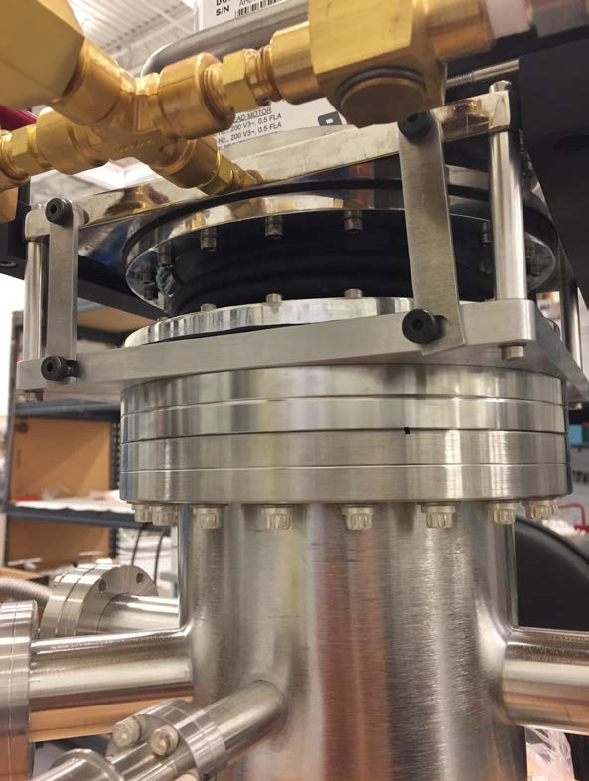
\includegraphics[width=0.5\linewidth]{fig_3_exchange_gas_space.pdf}
    \caption{Exchange gas space.}
    \label{fig:exchange_gas_space}
\end{figure}

The model of this cryostat is SHI-4XG-15-UHV, designed and manufactured by Janis Inc \cite{RN121}. In order to reduce vibration, we provide some design suggestions. The cryostat consists of a cold head, an exchange gas space and a vacuum chamber.
The cold head is powered by a helium compressor. The models of cold head and helium compressor are RDK-415D2 and F70-H produced by Sumitomo Corporation of Japan. The cold head features two stages with different refrigeration capacity: the 40 K stage has $\sim$ 35 W, and the 4 K stage has 1.5 W, as shown in Table~\ref{tab:refrigeration_capacity}. The cold head must be fixed near the vacuum chamber, but there are only three interfaces of the cold head: the power supply, the supply high-pressure helium tube and the return high-pressure helium tube. Therefore, we place the helium compressor and water cooler in the grey room of the laboratory to further isolate the source of vibration noise. The single continuous running time of the cold head can exceed 10,000 hours, which is enough for us to carry out long-term experiments.

\begin{table}
    \centering
    \caption{Refrigeration capacity (typical).}
    \begin{tabular}{p{0.2\linewidth}p{0.3\linewidth}p{0.3\linewidth}}
        \toprule
                     & RDK-408D2                   & RDK-415D2                   \\
        \midrule
        First stage  & 40 Watts @ 43 K (50 Hz)     & 35 Watts @ 50 K (50 Hz)     \\
                     & 50 Watts @ 43 K (60 Hz)     & 45 Watts @ 50 K (60 Hz)     \\
        Second stage & 1.0 Watt @ 4.2 K (50/ 60Hz) & 1.5 Watt @ 4.2 K (50/60 Hz) \\
        \bottomrule
    \end{tabular}
    \label{tab:refrigeration_capacity}
\end{table}

The exchange gas space, as shown in Fig~\ref{fig:exchange_gas_space}, is mainly composed of rubber bellow, helium pressure gauge and some helium valves. The top side and bottom side of the exchange gas space are respectively connected to the cold head and the vacuum chamber. The role of bellow is to reduce the vibration generated by the cold head and directly transmitted to the vacuum chamber, because rubber is more elastic than stainless steel. I think it is worth trying to replace the rubber bellow with a stainless-steel sheet that has been bent many times, because using a rubber bellow may cause leakage in the long-term operation of the system. Leakage of rubber bellow may come from three aspects. Firstly, the rubber material will deteriorate after a long-time operation. Our system has a leakage problem after about 2 years of operation, which is manifested as water inside the exchange gas space after the process of cooling down and warming up. Secondly, the rubber bellow is prone to defects during machining. We have contacted our supplier to process a new rubber bellow after we found the leakage problem, and notice that some of the rubber bellow had defects on the surface during many attempts. Finally, the sealing method of rubber bellow is worse than that of stainless steel. Our cryostat uses o-ring to seal rubber bellow \cite{RN133}. We tried to have the supplier process different rubber bellow to test the leakage, such as testing different materials and thickness of rubber bellow. In some poor cases, after a single cooling and reheating process will appear leakage, we finally used silicone rubber bellow and the thickness is twice the original and no leakage has been found so far.



\section{Cryogenic and UHV system}

\begin{figure}
    \centering
    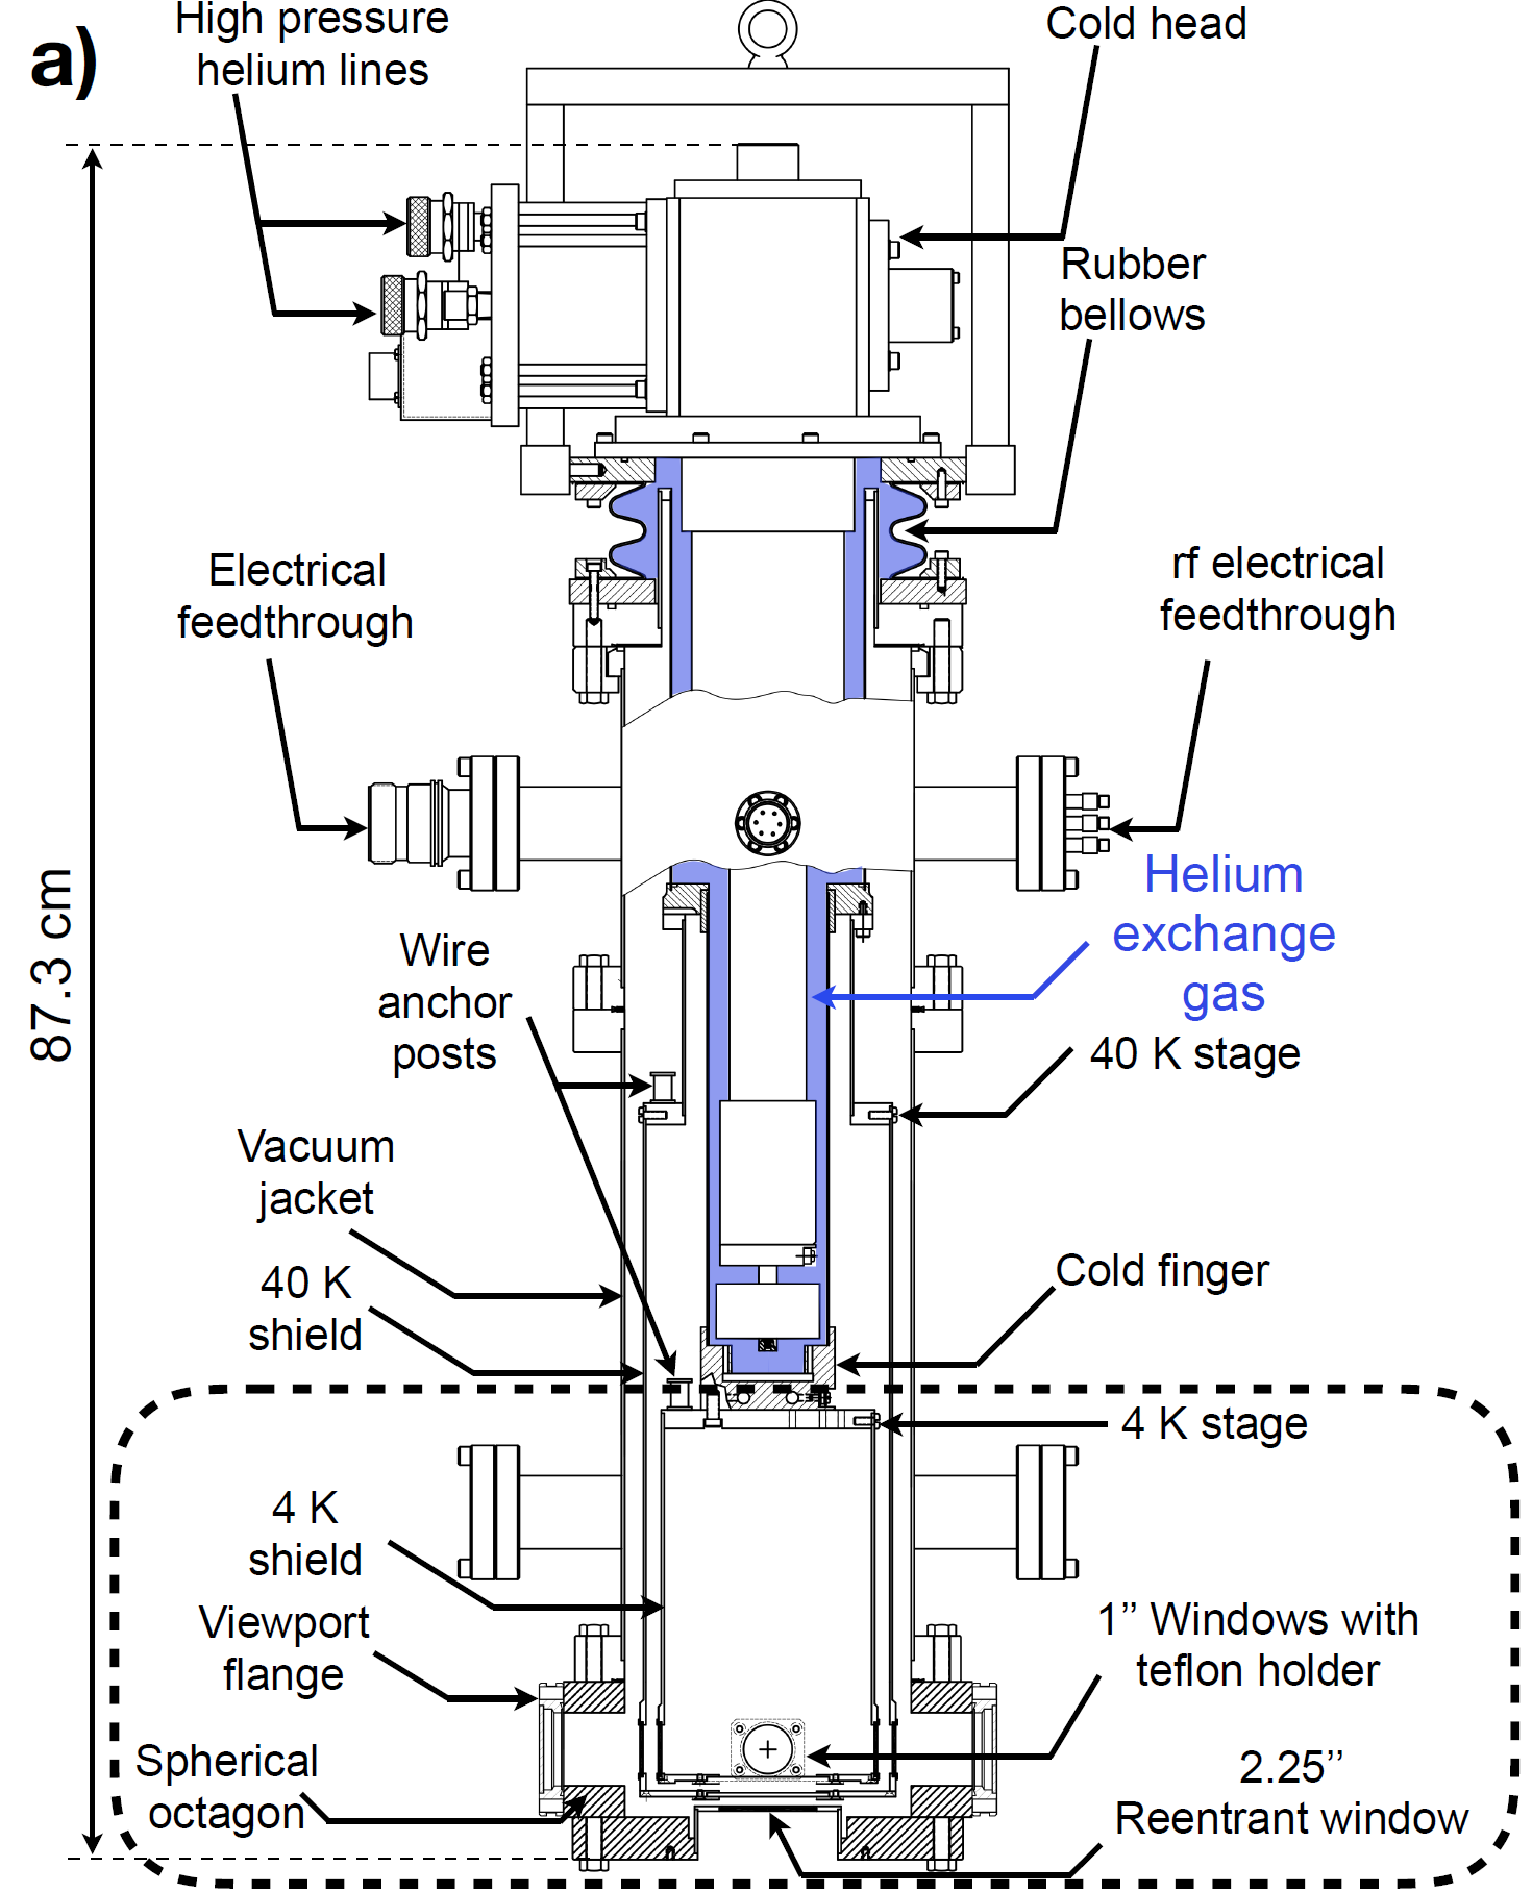
\includegraphics[width=0.7\linewidth]{fig_3_cryostat_a.pdf}
    \caption{The side section view of the Gilford-McMahon cryostat.}
    \label{fig:cryostat_a}
\end{figure}

The vacuum chamber resembles a cylinder with a diameter of about 200 mm and a height of about 600 mm. Externally, the upper part of the vacuum chamber has some feedthroughs connecting the electrical equipment to the vacuum equipment, and the lower part is a spherical octagon. The top of the vacuum chamber is in contact with the exchange gas space, and the bottom is the re-entrant window. In our experiments, we used a total of three electrical feedthroughs, one DC feedthrough to drive the voltage signal to the electrodes of the trap, another DC feedthrough to drive the thermometer and heater in the vacuum chamber, and an RF feedthrough to drive the RF signal to the resonator. Below them, there are a total of three Vacuum feedthroughs. One connected to an ion gauge (Agilent UHV-24P) to monitor the vacuum level in the vacuum chamber. One connected to a NEG-Ion pump (SAES NextTorr Z100) to pump out hydrogen, since hydrogen is the least efficiently cryo-pumped gas. And an angle valve is used to pump out vacuum during system maintenance. A spherical octagon holds eight 1'' diameter windows to provide optical access in the horizontal plane. These windows are made of UVFS and have different wavelength optical coatings according to the optical path design. We replaced one of the windows along the trap axis with an oven feedthrough, and installed both enriched ${ }^{171} \mathrm{Yb}$ oven and enriched ${ }^{174} \mathrm{Yb}$ oven on it, and finally tested them to work. However, assembly errors during installation may cause the ytterbium flux cannot enter the trap during ion loading. we can increase the translation degrees of freedom when designing the part to solve this problem. According to our experience, because of the large divergence angle of ytterbium flux, we just need to be able to see the trap and oven through the opposite window. The re-entrant window located at the bottom of the vacuum chamber has a diameter of 2.25'', below which is the imaging system. The maximum numerical aperture allowed for imaging ions along the vertical direction is 0.5. The Re-entrant window is surrounded by a doughnut-shaped aluminum base placed on an optical breadboard, and the base carries the full weight of the vacuum chamber. We tried to fasten between the upper part of the vacuum chamber and the optical breadboard with an aluminum sloped beam, but it did not reduce the vibration of the trap, indicating that the current support structure is solid enough.

\begin{table}
    \centering
    \caption{Table of electrical devices connected to the vacuum chamber.}
    \begin{tabular}{ll}
        \toprule
        Device                 & Model                      \\
        \midrule
        Ion gauge              & Agilent UHV-24P            \\
        NEG-Ion pump           & SAES NextTorr Z100         \\
        Temperature controller & CryoCon Model 26           \\
        DC signal source       & Homemade 16-channel AD5791 \\
        RF signal source       & Rohde \& Schwarz SMB-100B  \\
        \bottomrule
    \end{tabular}
\end{table}

The main components inside the vacuum chamber are the 40 K shield, the 4 K shield and the sample mount. These two shields are used to shield the ion trap from room temperature blackbody radiation. Their material is aluminum, but copper may be a better choice because copper material has a higher thermal conductivity. The bottom of the two shields are eight 1" UVFS windows, which correspond to the spherical octagon and have the same optical coating. The glass is fixed in the groove by the Teflon holder in order to keep the windows from being crushed during the cooling procedure. However, because of the elasticity of Teflon, the positioning accuracy of the windows is poor, which may be the main source of optical aberration. The top of the 40 K shield is in contact with the 40 K stage of the cold head through the helium gas in the exchange gas space, which is usually higher than 40 K, we name it that way just because it is intuitive. The top of the 4 K shield is fixed to the sample mount, which is made of oxygen-free copper with a gold-plated surface to obtain a high thermal conductivity and to prevent oxidation during system maintenance. The sample mount and the 4 K stage of the cold head are separated by a heat exchanger and cryogenic helium gas. The 4 K stage can reach temperatures below 4 K, and the heat exchanger is composed of a series of concentric circular oxygen-free copper sheets, which are designed to increase the refrigeration capacity at the sample mount. However, if the position between a pair of heat exchangers is shifted during operation and touches each other, it can introduce large vibrations to the sample mount, for example when floating the optical table.

\begin{figure}
    \centering
    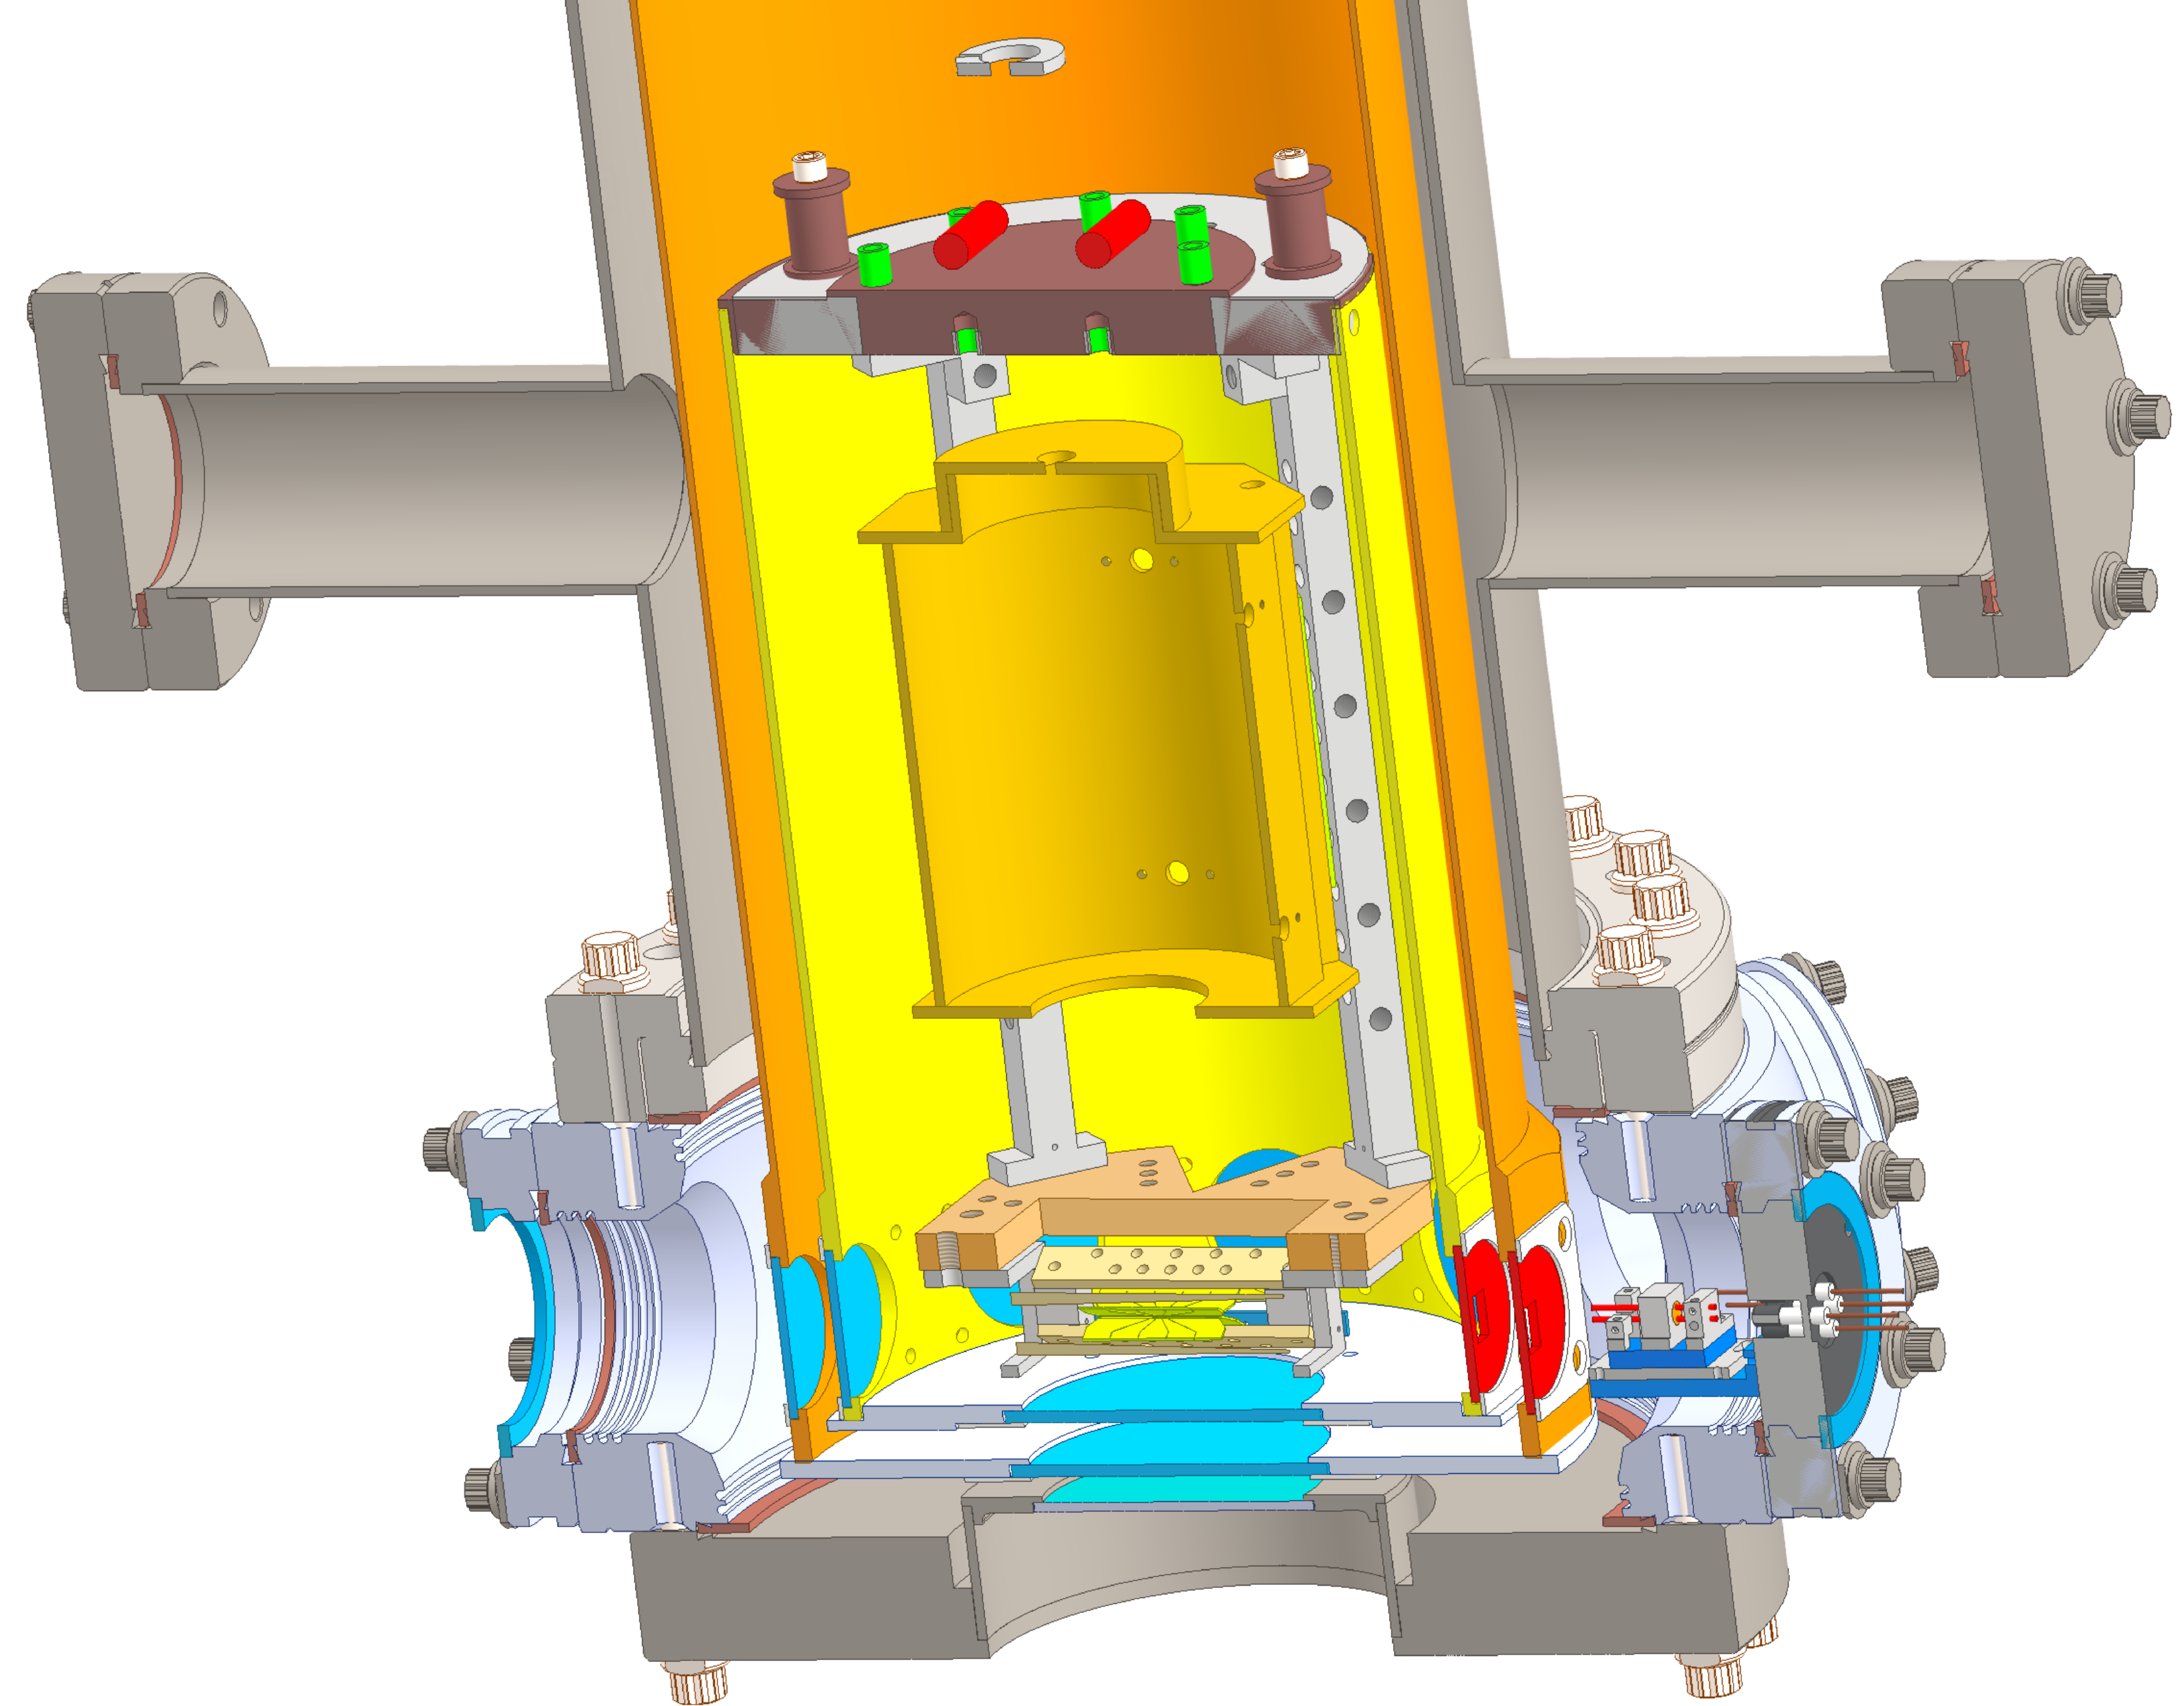
\includegraphics[width=0.7\linewidth]{fig_3_cryostat_b.pdf}
    \caption{The oblique view of ion trap and vacuum chamber.}
\end{figure}

Although the refrigeration capacity of the 4 K stage in the cold head reaches 1.5 W, the refrigeration capacity of the sample mount in the vacuum chamber, which is directly available to the user, is much lower. The reduction of the refrigeration capacity comes from the heat conduction between the 4 K stage and the sample mount and the heat leakage from the environment. In order to improve the heat transfer between the 4 K stage and the sample mount, we can increase the surface area of the heat exchanger. We can also fill the exchange gas space with sufficient helium gas, and it is necessary to use oxygen-free copper to produce thermally conductive parts. In our experiments, we use auto gas charging system to stabilize the helium pressure in the exchange gas space at a fixed positive pressure. It is worth noting that the rubber bellow loses its vibration isolation function under negative pressure, and the life of the rubber bellow is reduced.

\begin{figure}
    \centering
    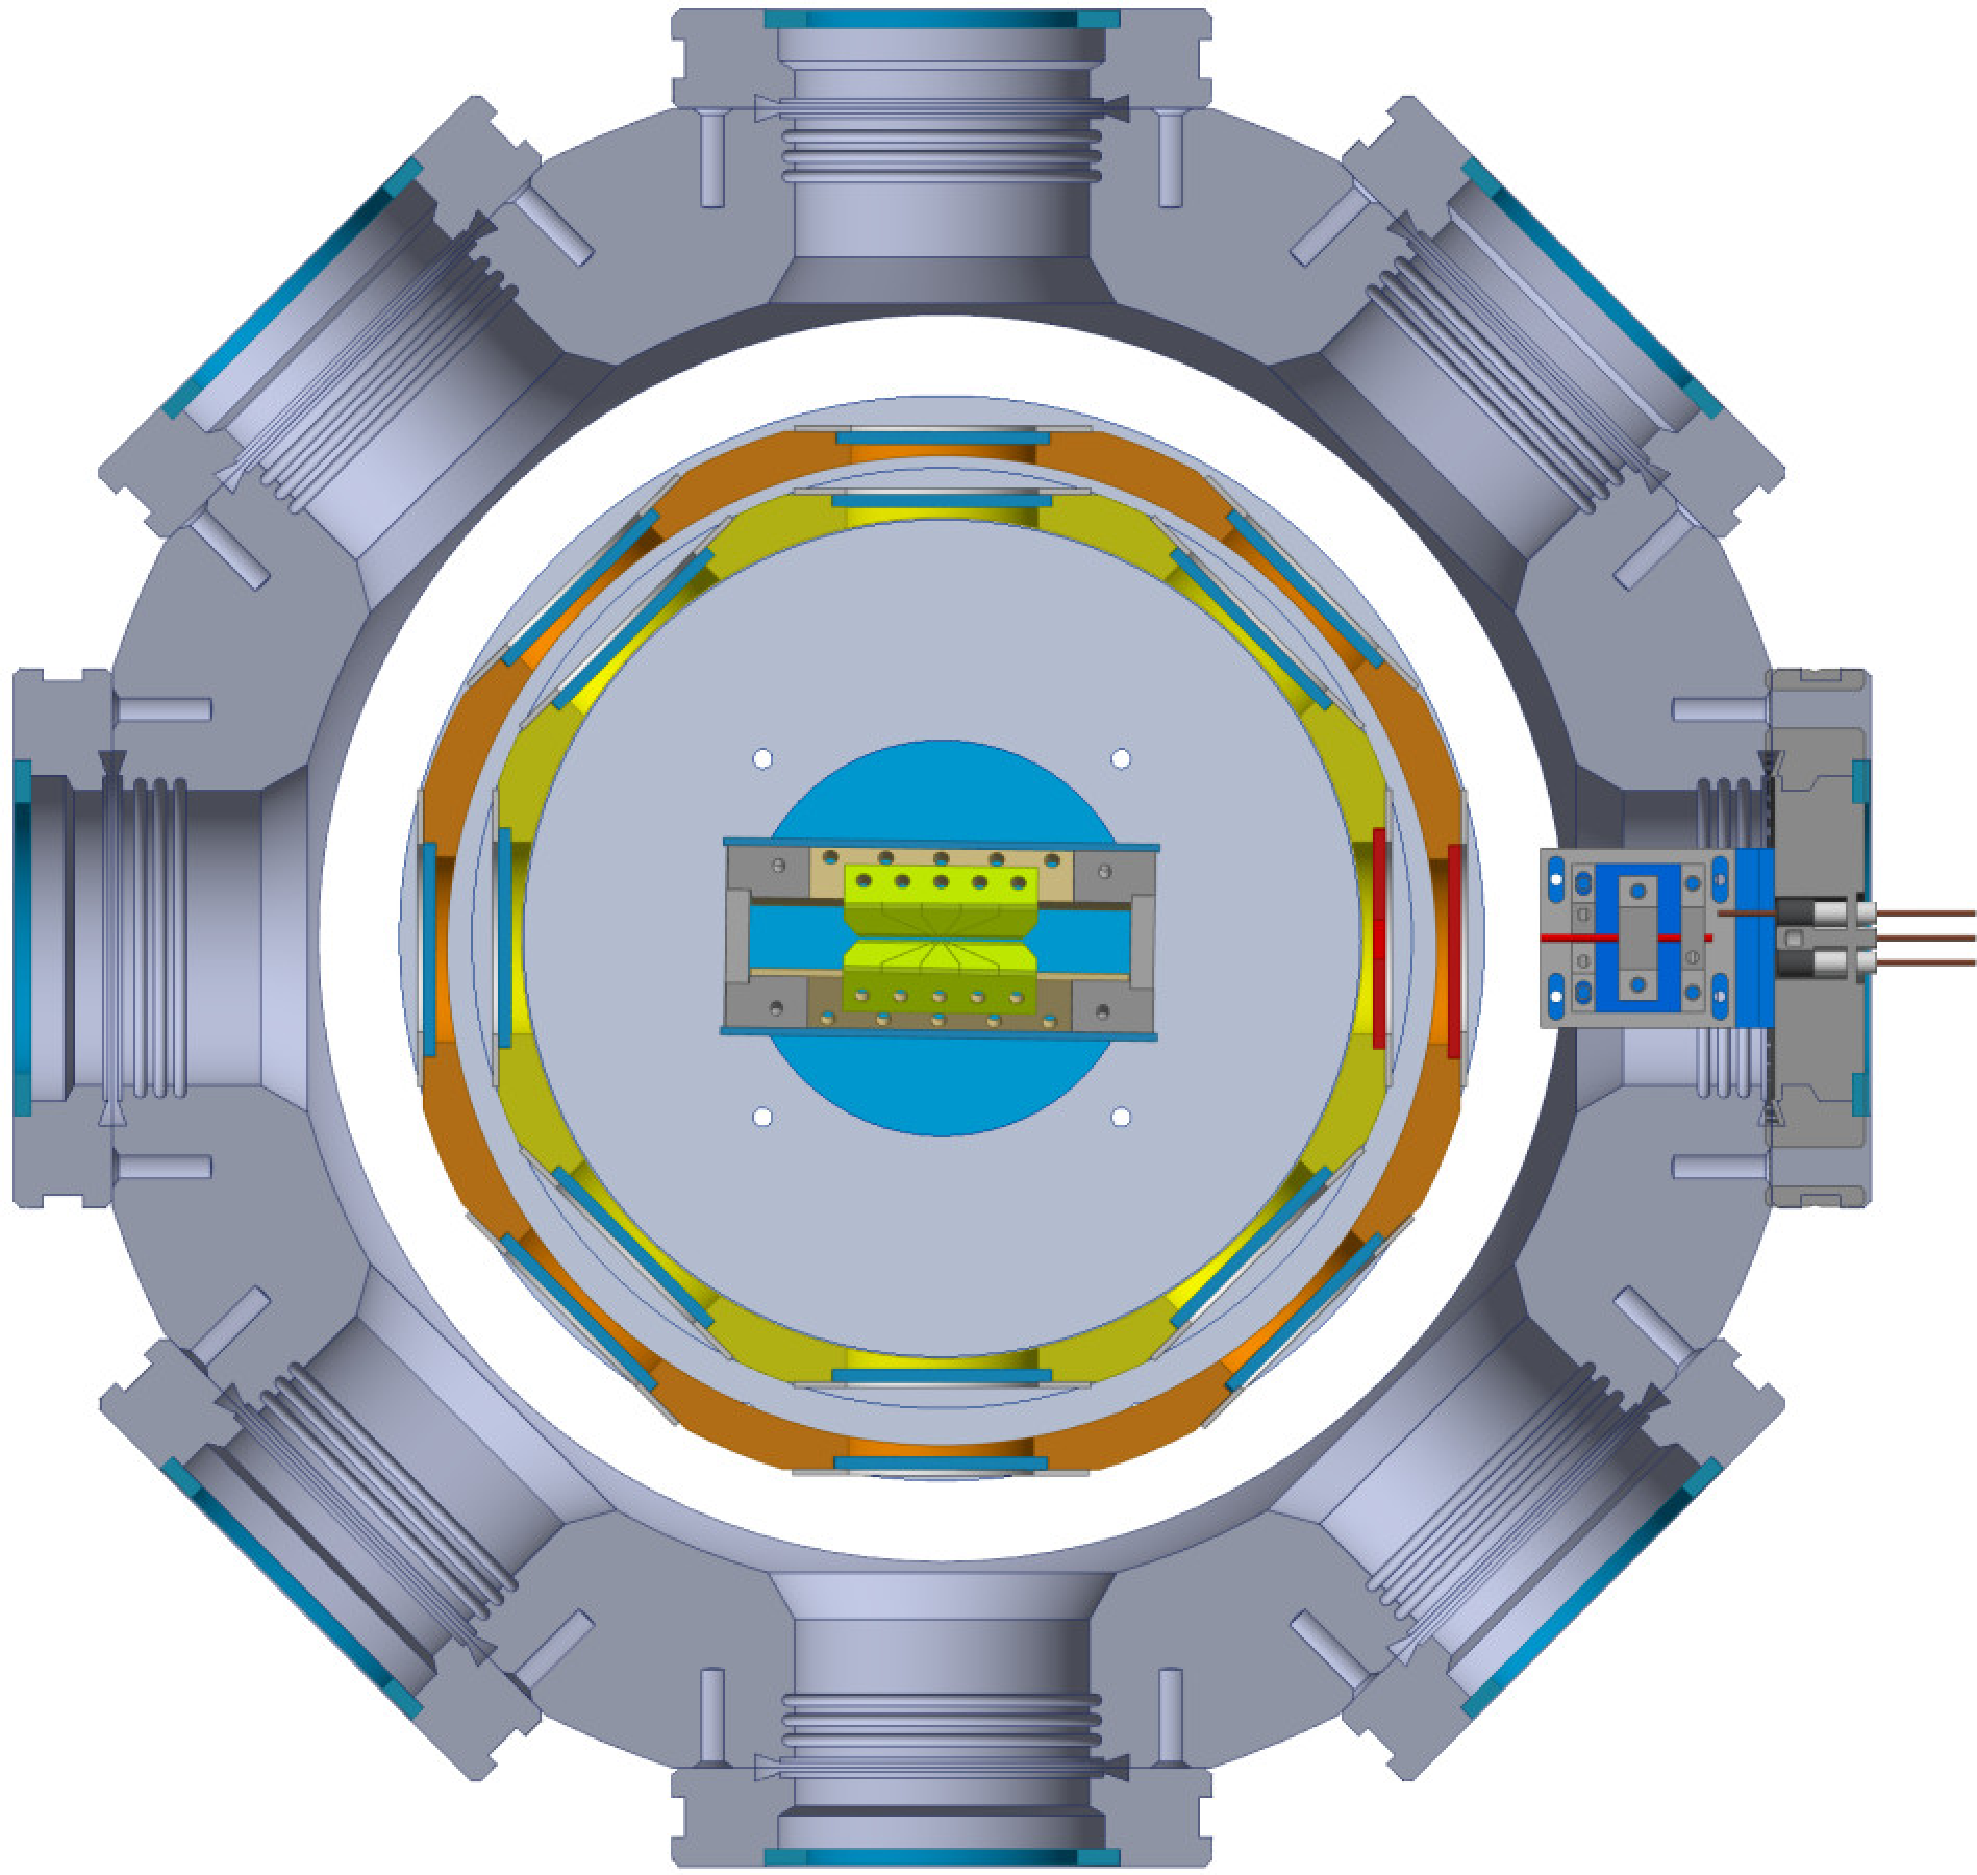
\includegraphics[width=0.7\linewidth]{fig_3_cryostat_c.pdf}
    \caption{The top view of ion trap and vacuum chamber.}
\end{figure}

The auto gas charging system was designed by PHYSIK and is based on the principle of using a PLC to read the helium pressure gauge and control the opening and closing moments of the helium valves, which will eventually stabilize the helium pressure gauge at 1.03 bar. There are two helium valves to control the helium inlet and outlet, and one safety value to allow excess helium to escape, preventing the bellow from bursting when the auto gas charging system is not working. The temperature stabilize system is a kit we purchased from Janis Inc. and consists of a thermometer, heater and temperature controller. The thermometer (DT-670-CU-HT-1.4H) is located inside the sample mount in the vacuum chamber and has a measurement range of 1.4-500 K, covering the cryostat operating range of approximately 4-300 K. The heater is a 25 $\Omega$ resistor very close to the thermometer. The DC lines of the heater and the thermometer are connected to the temperature controller (Model 26 from CryoCon) on the instrument rack via a DC feedthrough on the vacuum chamber. In low temperature operation, the temperature of the sample mount can be stabilized at $6 \pm 0.05$ K for a long time by setting the appropriate PID parameters, as shown in Fig~\ref{fig:cryostat_temperature}. The output power of the heater is about 350 mW, which means that the refrigeration capacity of the sample mount has a margin of 350 mW.

The auto gas charging system and the temperature stabilize system are the key systems for the long-term stability of the cryostat. Although the temperature of this cryostat has almost no drift, we can observe that the trap can shift $\pm 1$ $\mu$m during the experiment. The operation to avoid the effects of such position shifts by frequent calibration of the system parameters is very complicated, so this instability can be fatal for an experimental system. The long drift of the sample mount comes from the mechanical structure of the cryostat.

\begin{figure}
    \centering
    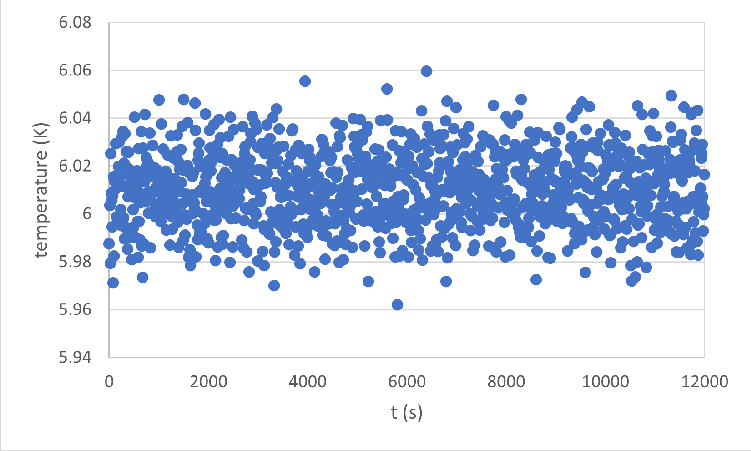
\includegraphics[width=0.7\linewidth]{fig_3_cryostat_temperature.pdf}
    \caption{The stablized temperature of the sample mount.}
    \label{fig:cryostat_temperature}
\end{figure}

The auto gas charging system can only stabilize the helium pressure near the rubber bellow, and the 40 K stage and 4 K stage of the cold head are not stabilized. Therefore, the pressure and temperature in the contact part of the vacuum chamber and the exchange gas space cannot be stabilized for a long time. However, this part is the support point of the sample mount, so the sample mount will be disturbed by these external environmental changes. We can consider fixing the sample mount to the room temperature area of the vacuum chamber, which will not move if the laboratory environment is stable, but this will inevitably increase the heat leakage from the room temperature area. In our experiments, we first pumped the vacuum chamber to $1 \times {10}^{-6}$ mbar at room temperature using the turbo pump, then activated the NEG-Ion pump for about 2 hours and at the end of the operation the vacuum chamber vacuum level dropped to $1 \times {10}^{-8}$ mbar. The vacuum chamber can reach a vacuum level of $3 \times {10}^{-10}$ mbar with the effect of the cryo-pump.



\section{Helical resonator and segmented blade trap}

The blade trap forms a capacitor of approximately 6 pF. In order to drive this capacitor, i.e. to apply a high voltage signal to it, we need a larger helical resonator to form the LC oscillation circuit and to achieve impedance matching \cite{RN267,RN262,RN263,RN308,RN265}. The two components are therefore closely linked. The helical resonator and the blade trap are both located inside the 4 K shield of the vacuum chamber. The helical resonator is fixed underneath the sample mount and then the blade trap is fixed underneath the helical resonator \cite{RN92,RN258,RN286,RN345}. This ensures that the helical resonator and the blade trap are very close to each other and that their temperatures are equally stable. At the same time the low temperature allows the resistance in the oscillator circuit to be significantly reduced, which helps to increase the quality factor of the oscillator circuit. The helical resonator and the blade trap are used as a single unit and its input and output are achieved via RF and DC electric feedthrough \cite{RN266}.

\subsection{Design of helical resonator}

\begin{figure}
    \centering
    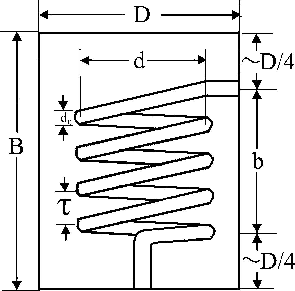
\includegraphics[width=0.5\linewidth]{fig_3_outline_design_of_a_helical_resonator.pdf}
    \caption{The outline design of a helical resonator.}
    \label{fig:outline_design_of_a_helical_resonator}
\end{figure}

The circuit models for the helical resonator and the blade trap have been well studied \cite{RN264,RN91,RN288}. In practice, we have developed a very mature design procedure with a high quality factor, choosing only two parameters $ b / d $ and $ d / D $ to optimise the performance of the helical resonator with the quality factor as the objective function. We can calculate the loading frequency in the empirical parameter regime using the trap capacitance and the quality factor. Typically, $ b / d \approx 1.5 $ and $ d / D \approx 0.5 $ are a good choice, and if the loading frequency meets our requirements, we will try to choose the highest quality factor around this parameter range, as shown in Fig~\ref{fig:outline_design_of_a_helical_resonator}. A two-wire spiral resonator is much more complex than a single-wire spiral resonator because of the coupling between the two coils. However, for the sake of simplicity, we are still using the model and we can achieve an accuracy of about $\pm 5$ MHz. To ensure that the phase and amplitude of the two coils are the same, we use a parallel capacitor, which is shorted when connected to the RF feedthrough, with a capacitance of approximately 300 nF. The two-wire design is designed to help minimize micromotion by applying a DC voltage to the RF electrodes, so we need to ensure that the RF signal on the coil is grounded and the DC voltage is not, this is achieved by a 300 nF capacitor connected to the shield. In addition, we added an RC filter before the DC voltage was connected to the coil.

\subsection{Circuit diagrams of the helical resonator and the blade trap}

\begin{figure}
    \centering
    \subcaptionbox{Circuit diagrams of the helical resonator.\label{fig:circuit_diagram_helical_resonator}}
    {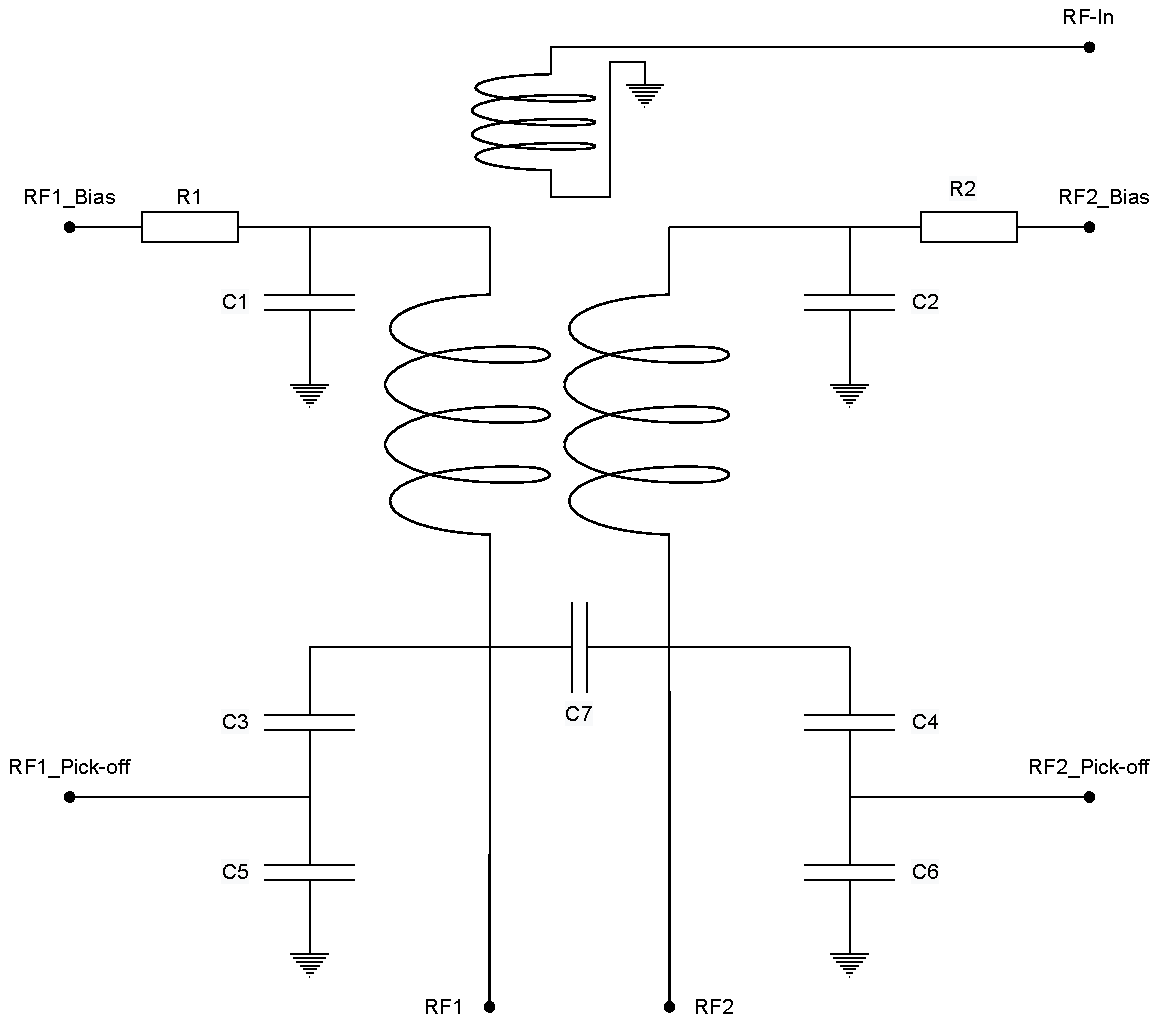
\includegraphics[width=0.5\linewidth]{fig_3_circuit_diagram_helical_resonator.pdf}}
    \subcaptionbox{Circuit diagrams of the blade trap.\label{fig:circuit_diagram_blade_trap}}
    {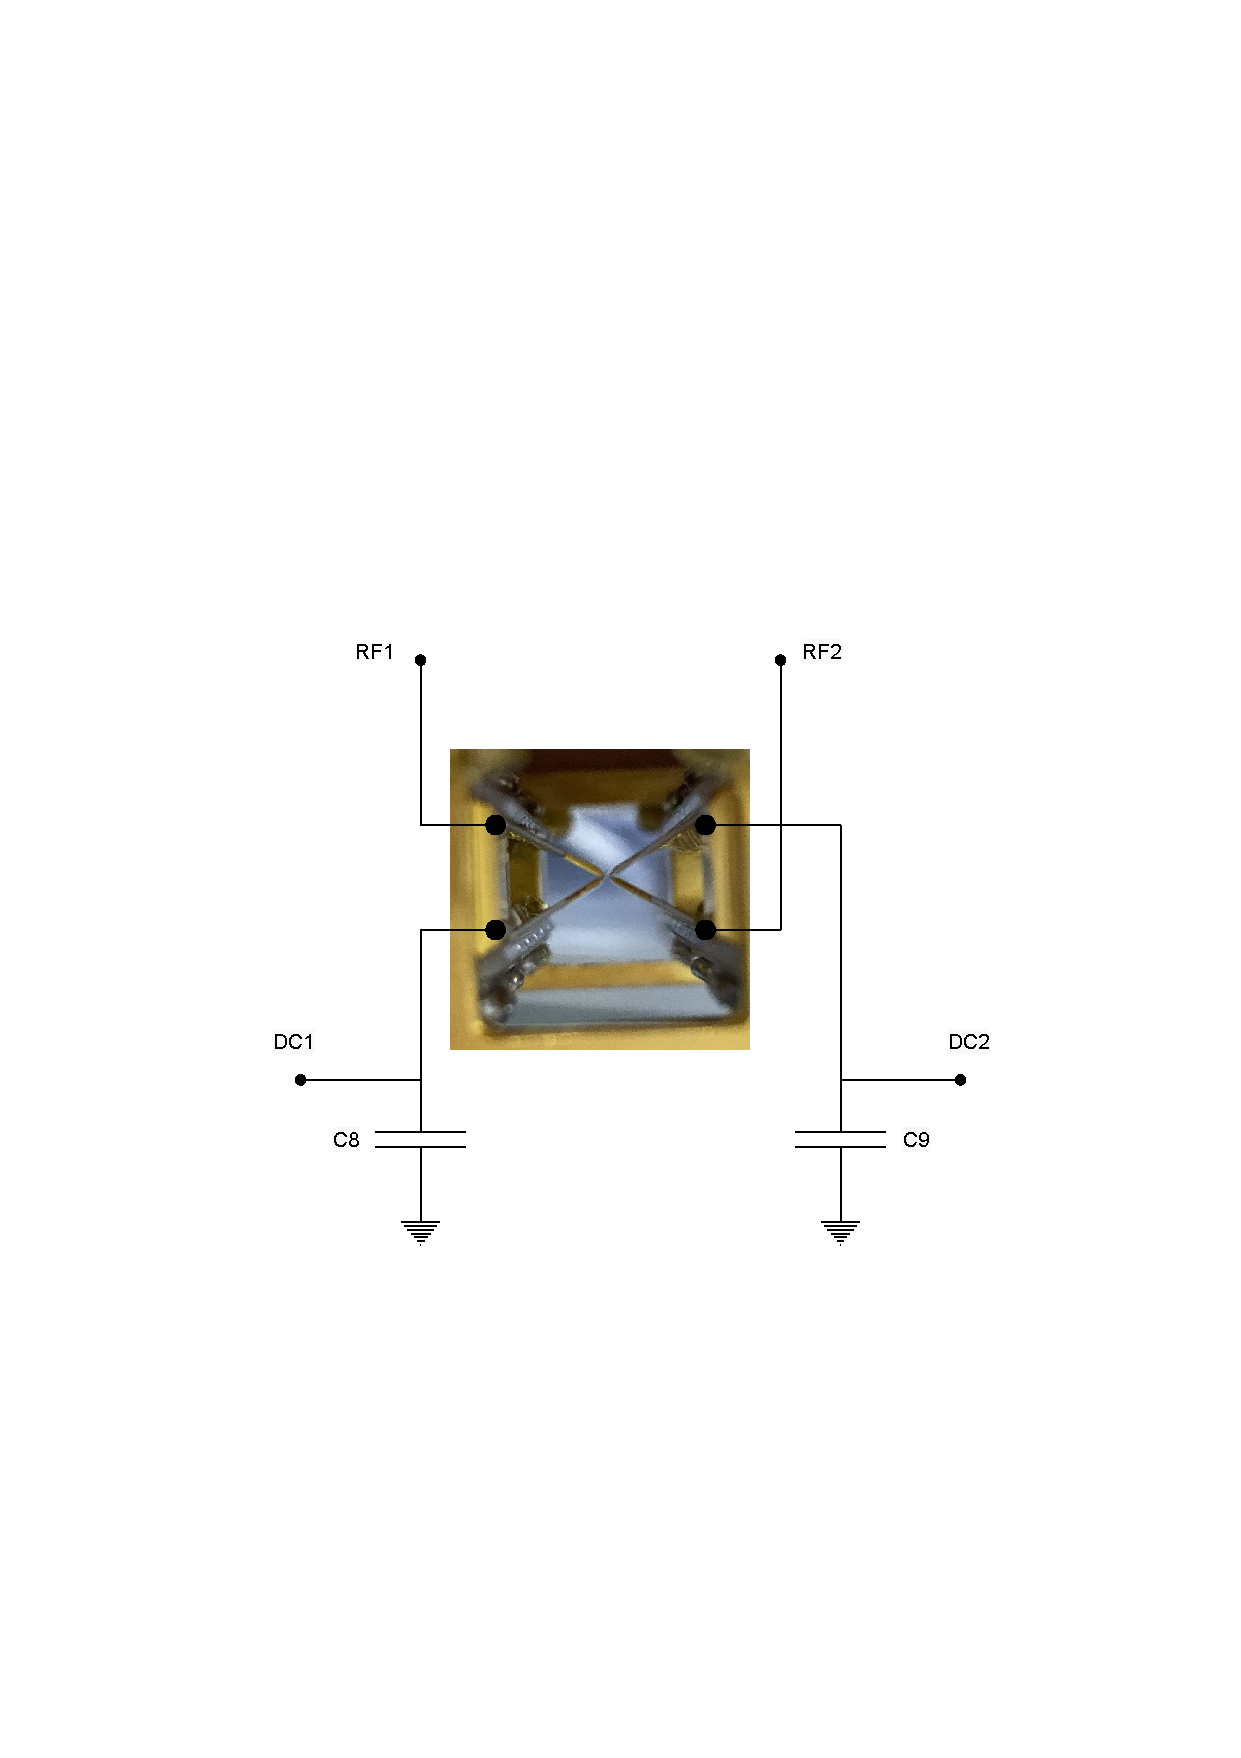
\includegraphics[width=0.3\linewidth]{fig_3_circuit_diagram_blade_trap.pdf}}
    \caption{Circuit diagrams of the helical resonator and the blade trap.}
    \label{fig:circuit_diagram}
\end{figure}

To facilitate our understanding of the circuit structure of the helical resonator and the blade trap, Fig~\ref{fig:circuit_diagram_helical_resonator} shows their equivalent circuit diagrams \cite{RN335,RN338}. In Fig~\ref{fig:circuit_diagram_blade_trap}, an external RF signal (RF-In) is fed to a small antenna. The antenna is coupled to a double bifilar helical copper wire, which is short-circuited by a large capacitor (C7; 330nF). The two RF bias signals (RF1 Bias and RF2 Bias) are supplied by the AD5791 and pass through an RC filter consisting of a resistor (R1, R2; 10 $k\Omega$) and a capacitor (C1, C2; 330 nF) to add a DC bias to the respective RF signal. The two capacitively coupled signals (RF1 Pick-off, RF2 Pick-off) can be coupled to a 1\% RF resonant signal. The voltage divider circuit uses a small capacitor (C3, C4; 0.2 pF) and a large capacitor (C5, C6; 20 pF) in series. The signal from the two pairs of DC electrodes on the blade trap (DC1, DC2) is grounded through large capacitors (C8, C9; 820 pF).

\begin{table}
    \centering
    \caption{Table of electronic components in the circuit diagrams.}
    \begin{tabular}{p{0.15\linewidth}p{0.1\linewidth}p{0.3\linewidth}p{0.3\linewidth}}
        \toprule
        Component & Value        & Model            & Parameters                   \\
        \midrule
        Resistor  & 10 $k\Omega$ & RNCF1206TKY10K0  & RES 10K OHM 0.01\% 1/4W 1206 \\
        Capacitor & 0.2 pF       & VJ1111D0R2VXRAJ  & 1.5KV                        \\
        Capacitor & 20 pF        & 800B200JT500XT   & CAP CER  500V C0G/NP0 1111
        \\
        Capacitor & 820 pF       & C0805C821JCGACTU & CAP CER  500V C0G/NP0 0805   \\
        Capacitor & 330 nF       & C2220C334J1GACTU & 100V NP0
        \\
        \bottomrule
    \end{tabular}
\end{table}

\subsection{Assembly of the helical resonator}

The material used for the body of the helical resonator is oxygen-free copper, which is characterised by its very low resistivity and high thermal conductivity. The low resistivity helps to obtain a high quality factor, but the oxygen-free copper is susceptible to oxidation during processing, so the oxide film needs to be removed before assembly. After the helical resonator has been assembled, it needs to be placed in a vacuum enclosure to prevent oxidation \cite{RN333,RN337}.

\begin{figure}
    \centering
    \subcaptionbox{Assembly of the helical resonator antenna.\label{fig:assembly_of_helical_resonator_antenna}}
    {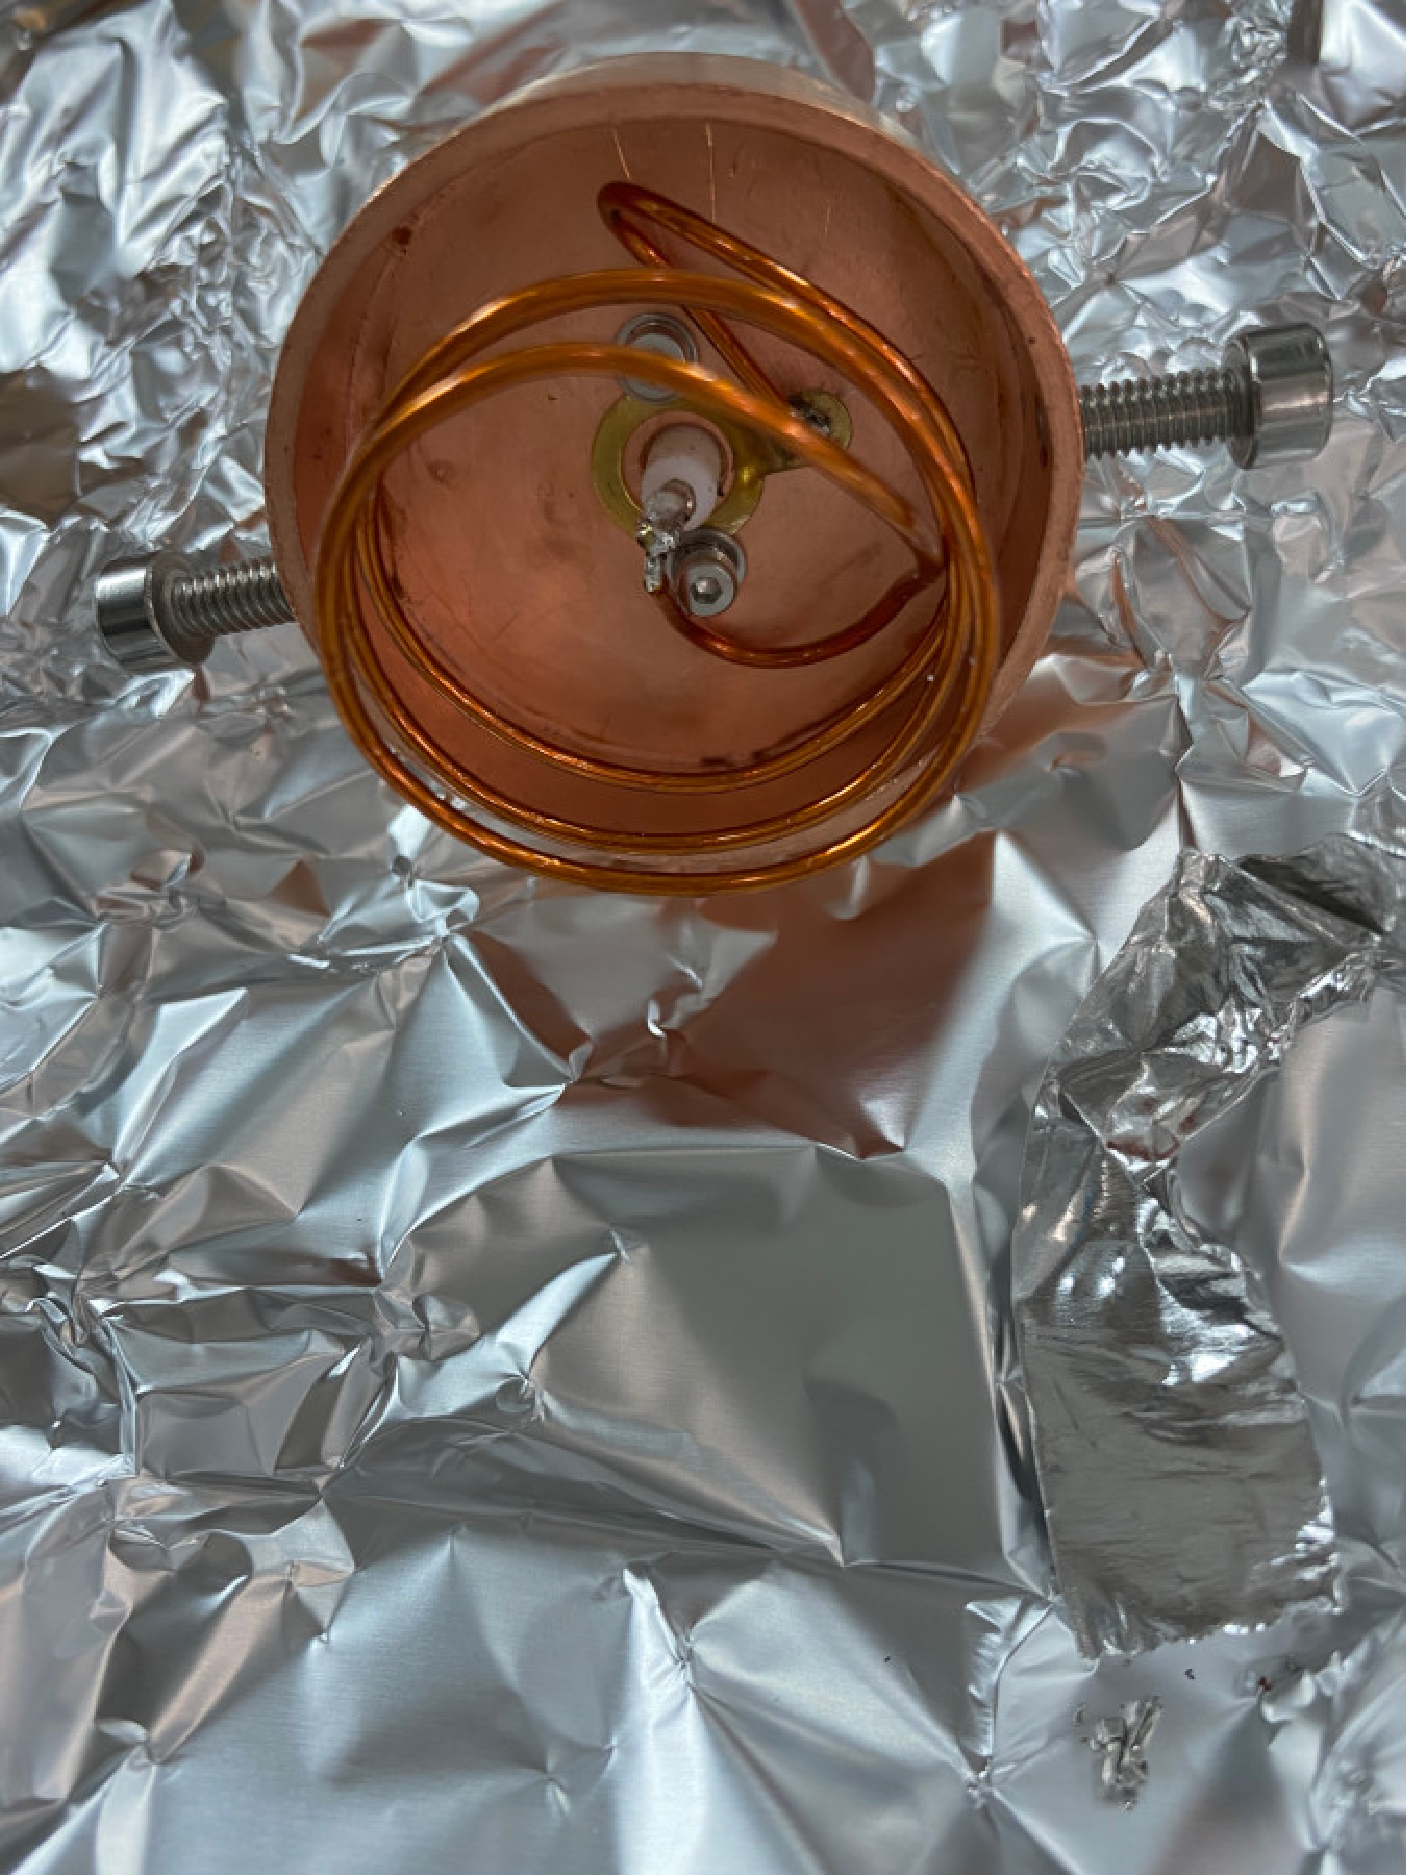
\includegraphics[width=0.4\linewidth]{fig_3_assembly_of_helical_resonator_antenna.pdf}}
    \subcaptionbox{Assembly of the main section.\label{fig:assembly_of_helical_resonator_copper}}
    {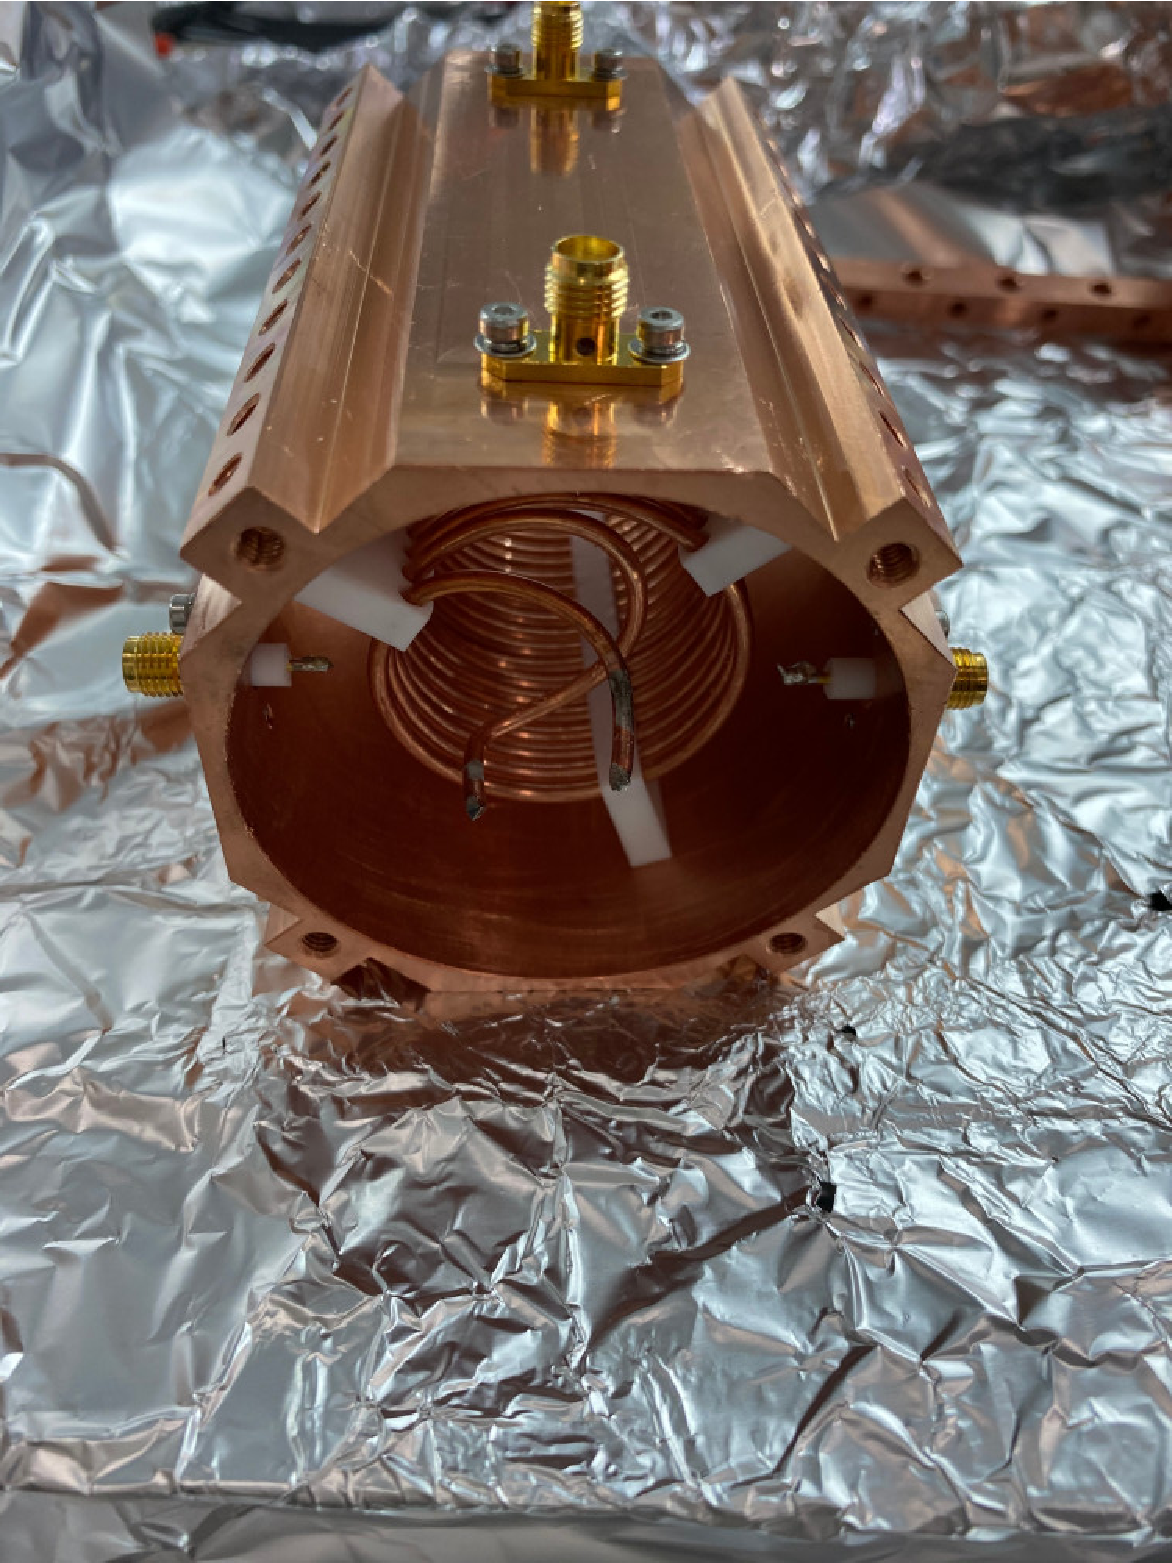
\includegraphics[width=0.4\linewidth]{fig_3_assembly_of_helical_resonator_copper.pdf}}
    \subcaptionbox{Assembly and soldering of the PCB.\label{fig:assembly_of_helical_resonator_pcb}}
    {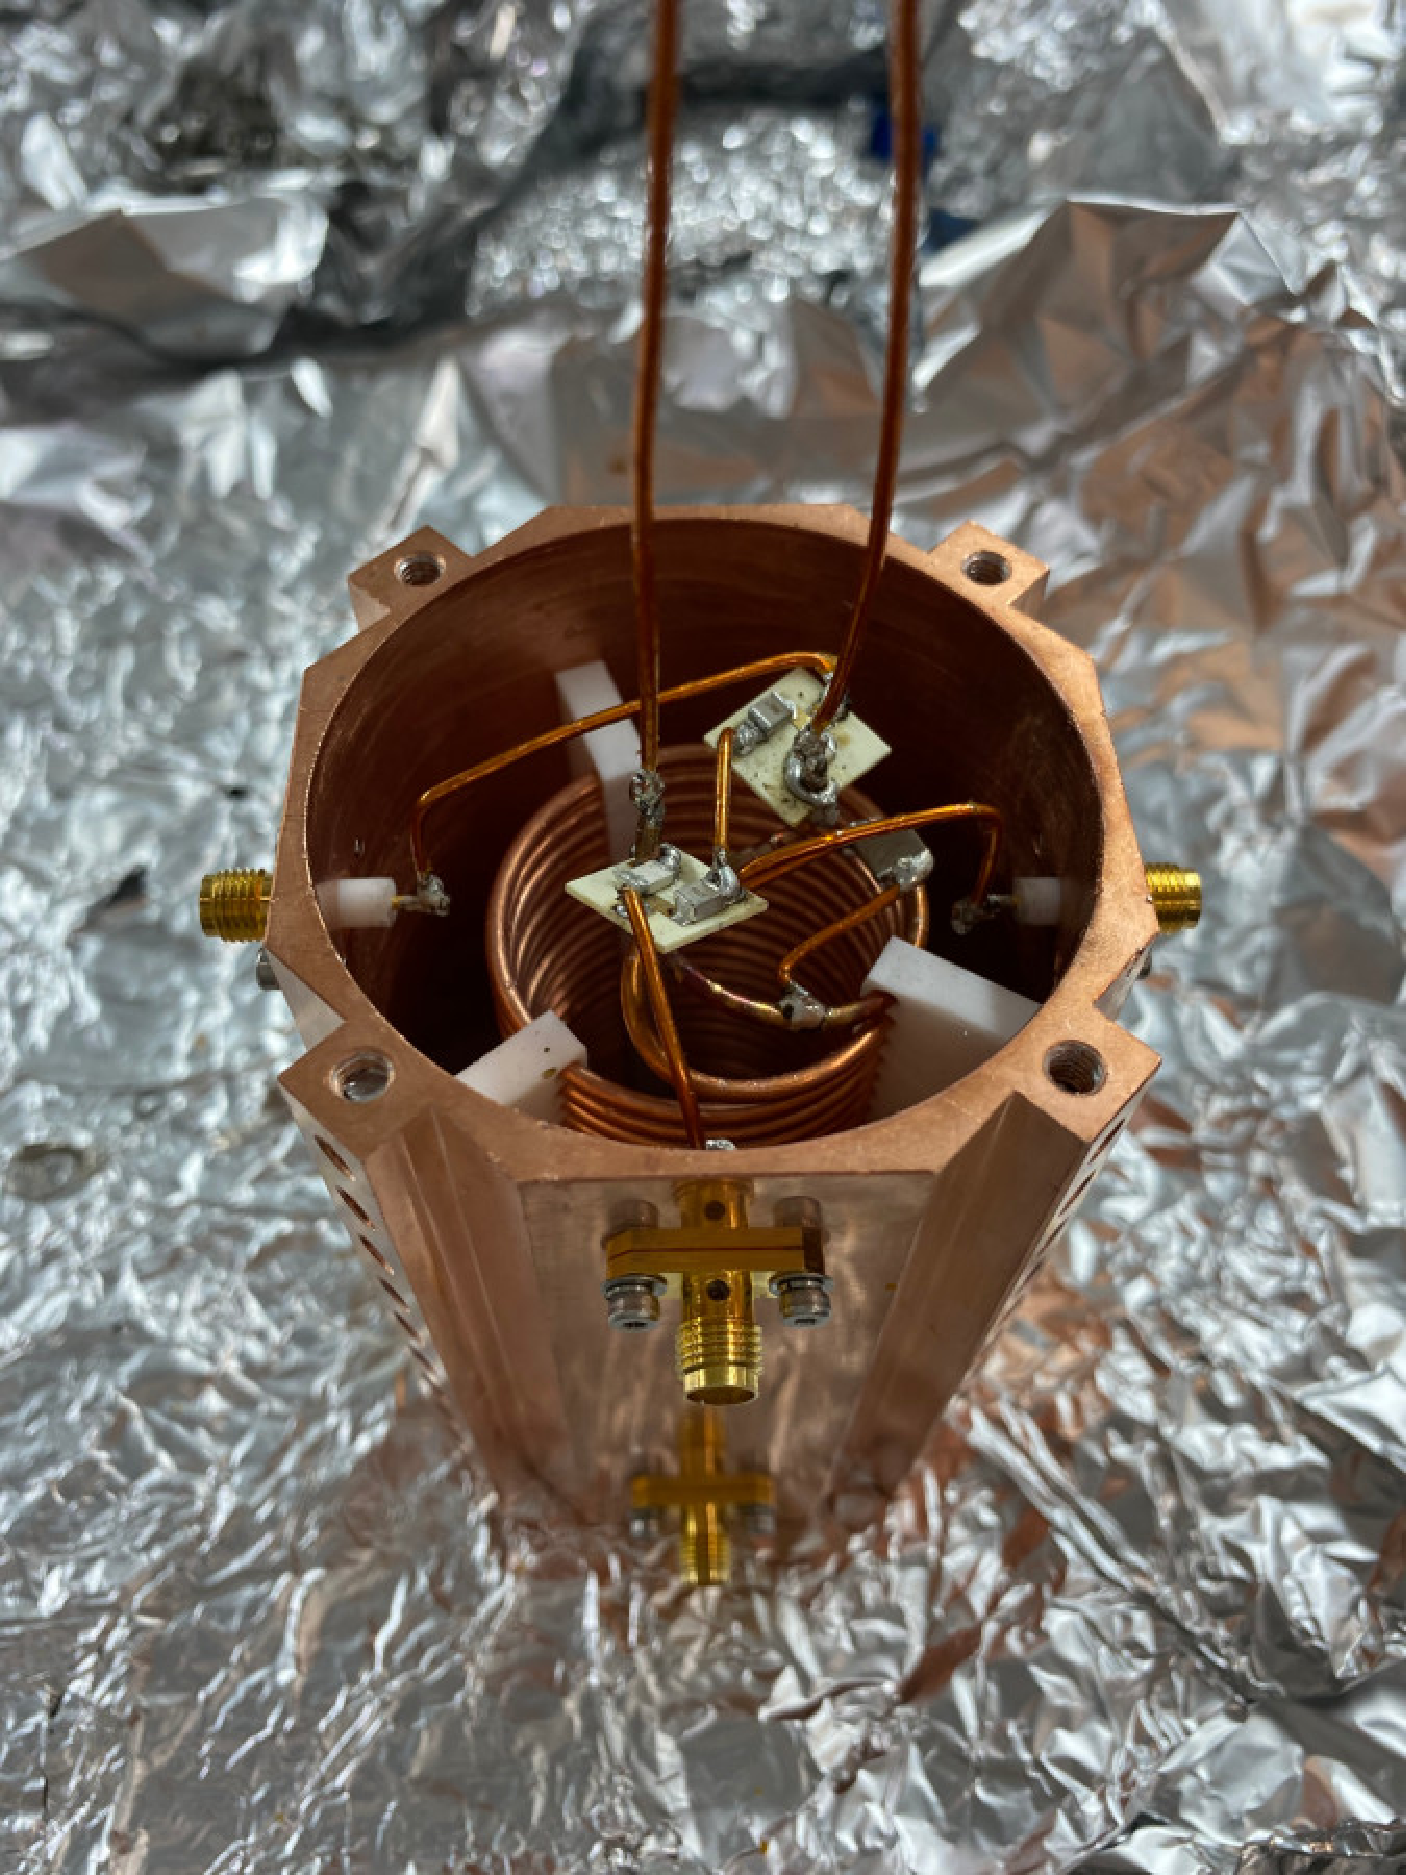
\includegraphics[width=0.5\linewidth]{fig_3_assembly_of_helical_resonator_pcb.pdf}}
    \caption{Assembly of the helical resonator.}
    \label{fig:assembly_of_helical_resonator}
\end{figure}

\begin{table}
    \centering
    \caption{Assembly procedures of the helical resonator.}
    \begin{tabular}{p{0.2\linewidth}p{0.7\linewidth}}
        \toprule
        Procedure    & Content                                                                                                                                                                                                                    \\

        \midrule
        Preservation & Oxygen-free copper components should not be left in the air for long periods of time and need to be placed in a vacuum enclosure.                                                                                          \\
        Clean        & Disassemble the helical resonator and take out the oxygen-free copper components individually into large beakers in preparation for sonication.                                                                            \\
                     & Sonicate them with acetone for 30 minutes and with ethanol for 5 minutes.                                                                                                                                                  \\
                     & Blow the components dry.                                                                                                                                                                                                   \\
                     & Soak them in organic acid for 5 minutes, where the surface oxide film can be observed to disappear and turn purplish red.                                                                                                  \\
                     & Remove residual organic acids from the surface by immerse them in plenty of distilled water.                                                                                                                               \\
                     & Wipe the surface of the oxygen-free copper components with paper, place them in a vacuum hood and evacuate the vacuum enclosure.                                                                                           \\
        Preparation  & Cut a number of thick wires into suitable length and trim off the insulation at both ends.                                                                                                                                 \\
                     & Prepare the PCB, capacitors, resistors, screw coil retainers, SMA connectors, copper plated components, indium foil, screw sets and spanners.                                                                              \\
                     & Soak the capacitors, resistors and indium foil in acetone for 30 minutes and in ethanol for 5 minutes and sonicate the rest in acetone for 30 minutes and in ethanol for 5 minutes.                                        \\
        Test         & Measure the inductance of the helical resonator with an LCR meter. (1.50 $\mu$H and 1.41 $\mu $H.)                                                                                                                         \\
                     & Measure the scattering parameters of the helical resonator with a vector network analyzer.                                                                                                                                 \\
                     & The antenna position and pitch were adjusted to match the impedance when the helical resonator was unloaded. (f = 69.15 MHz, Q = 434.7 U, R = 50.90 dB.)                                                                   \\
                     & After the helical resonator is connected to the Trap, the antenna position and pitch are adjusted so that the impedance matches, and at this point the RC filter is connected. (f = 36.83 MHz, Q = 373.6 U, R = 28.05 dB.) \\
        \bottomrule
    \end{tabular}
\end{table}

The main parts of the helical resonator were machined according to the design parameters: the antenna cover, the top cover, the middle part, the bottom cover and the helical coils, which were then cleaned in the ultrasound machine using acetone and ethanol. After drying these parts with nitrogen and soaking them in organic acid for 5 minutes, it can be observed that the surface oxide film disappears and turns purplish red. We soak the parts in plenty of distilled water to remove the residual organic acid and then dry the parts with nitrogen. The cleaning procedure of the whole parts of the the helical resonator's main section is now complete. This part needs to be done carefully, as the oxide film on the helical resonator surface affects the quality factor.

We also need to prepare and clean the rest of the parts according to the design parameters to meet the ultra-high vacuum requirements. We then solder the circuit components together using lead-free solder. The parts are then assembled with stainless steel screws, each requiring a resilient pad to prevent the screws from loosening at low temperatures.


\subsection{Assembly of blade trap}

The advantage of the blade trap is that it is easy to process and assemble, but the disadvantage is that the assembly error is higher compared to the surface trap or the monolithic trap, which causes an asymmetry in the electrostatic potential at the centre of the trap where the ions are located, i.e. a deviation from the linear trap configuration. When designing the blade trap for use in the cryostat, we need to take care that the material has a high thermal conductivity and that the connections between the components are sufficiently tight. In this way we can achieve the lowest temperatures on the blade trap. This helps to obtain a higher vacuum level and to extend the life of the ions.

\begin{figure}
    \centering
    \subcaptionbox{Assembly of the sapphire and indium film.}
    {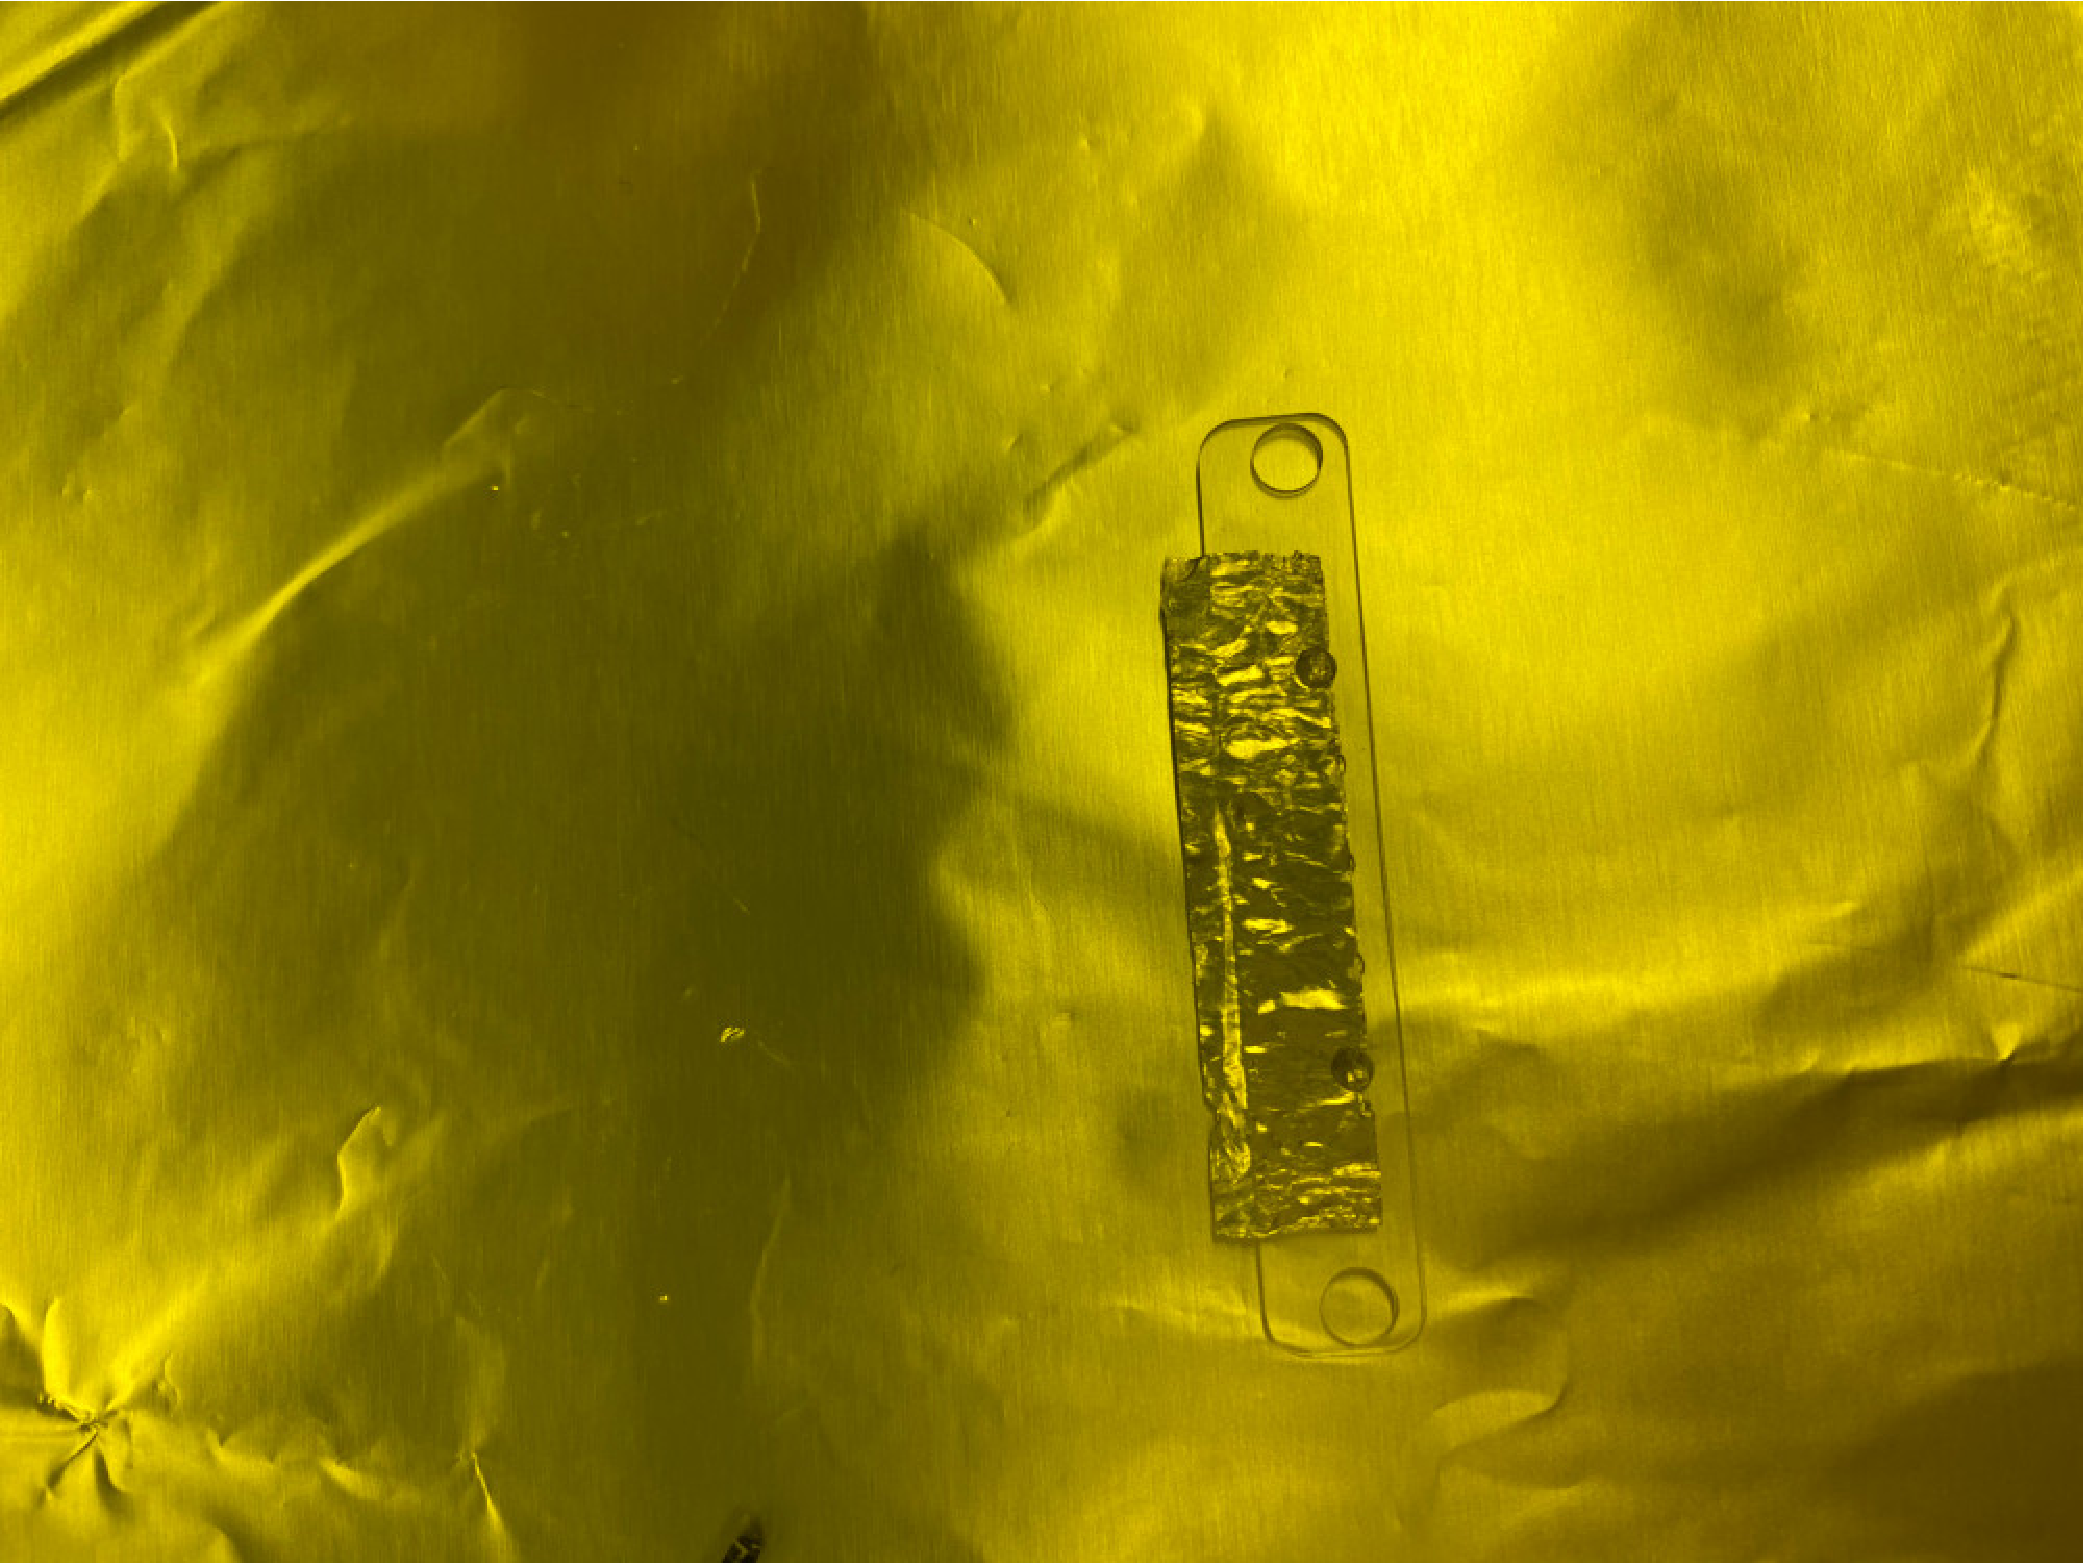
\includegraphics[width=0.4\linewidth]{fig_3_assembly_of_trap_sapphire.pdf}}
    \subcaptionbox{Assembly of the blade.}
    {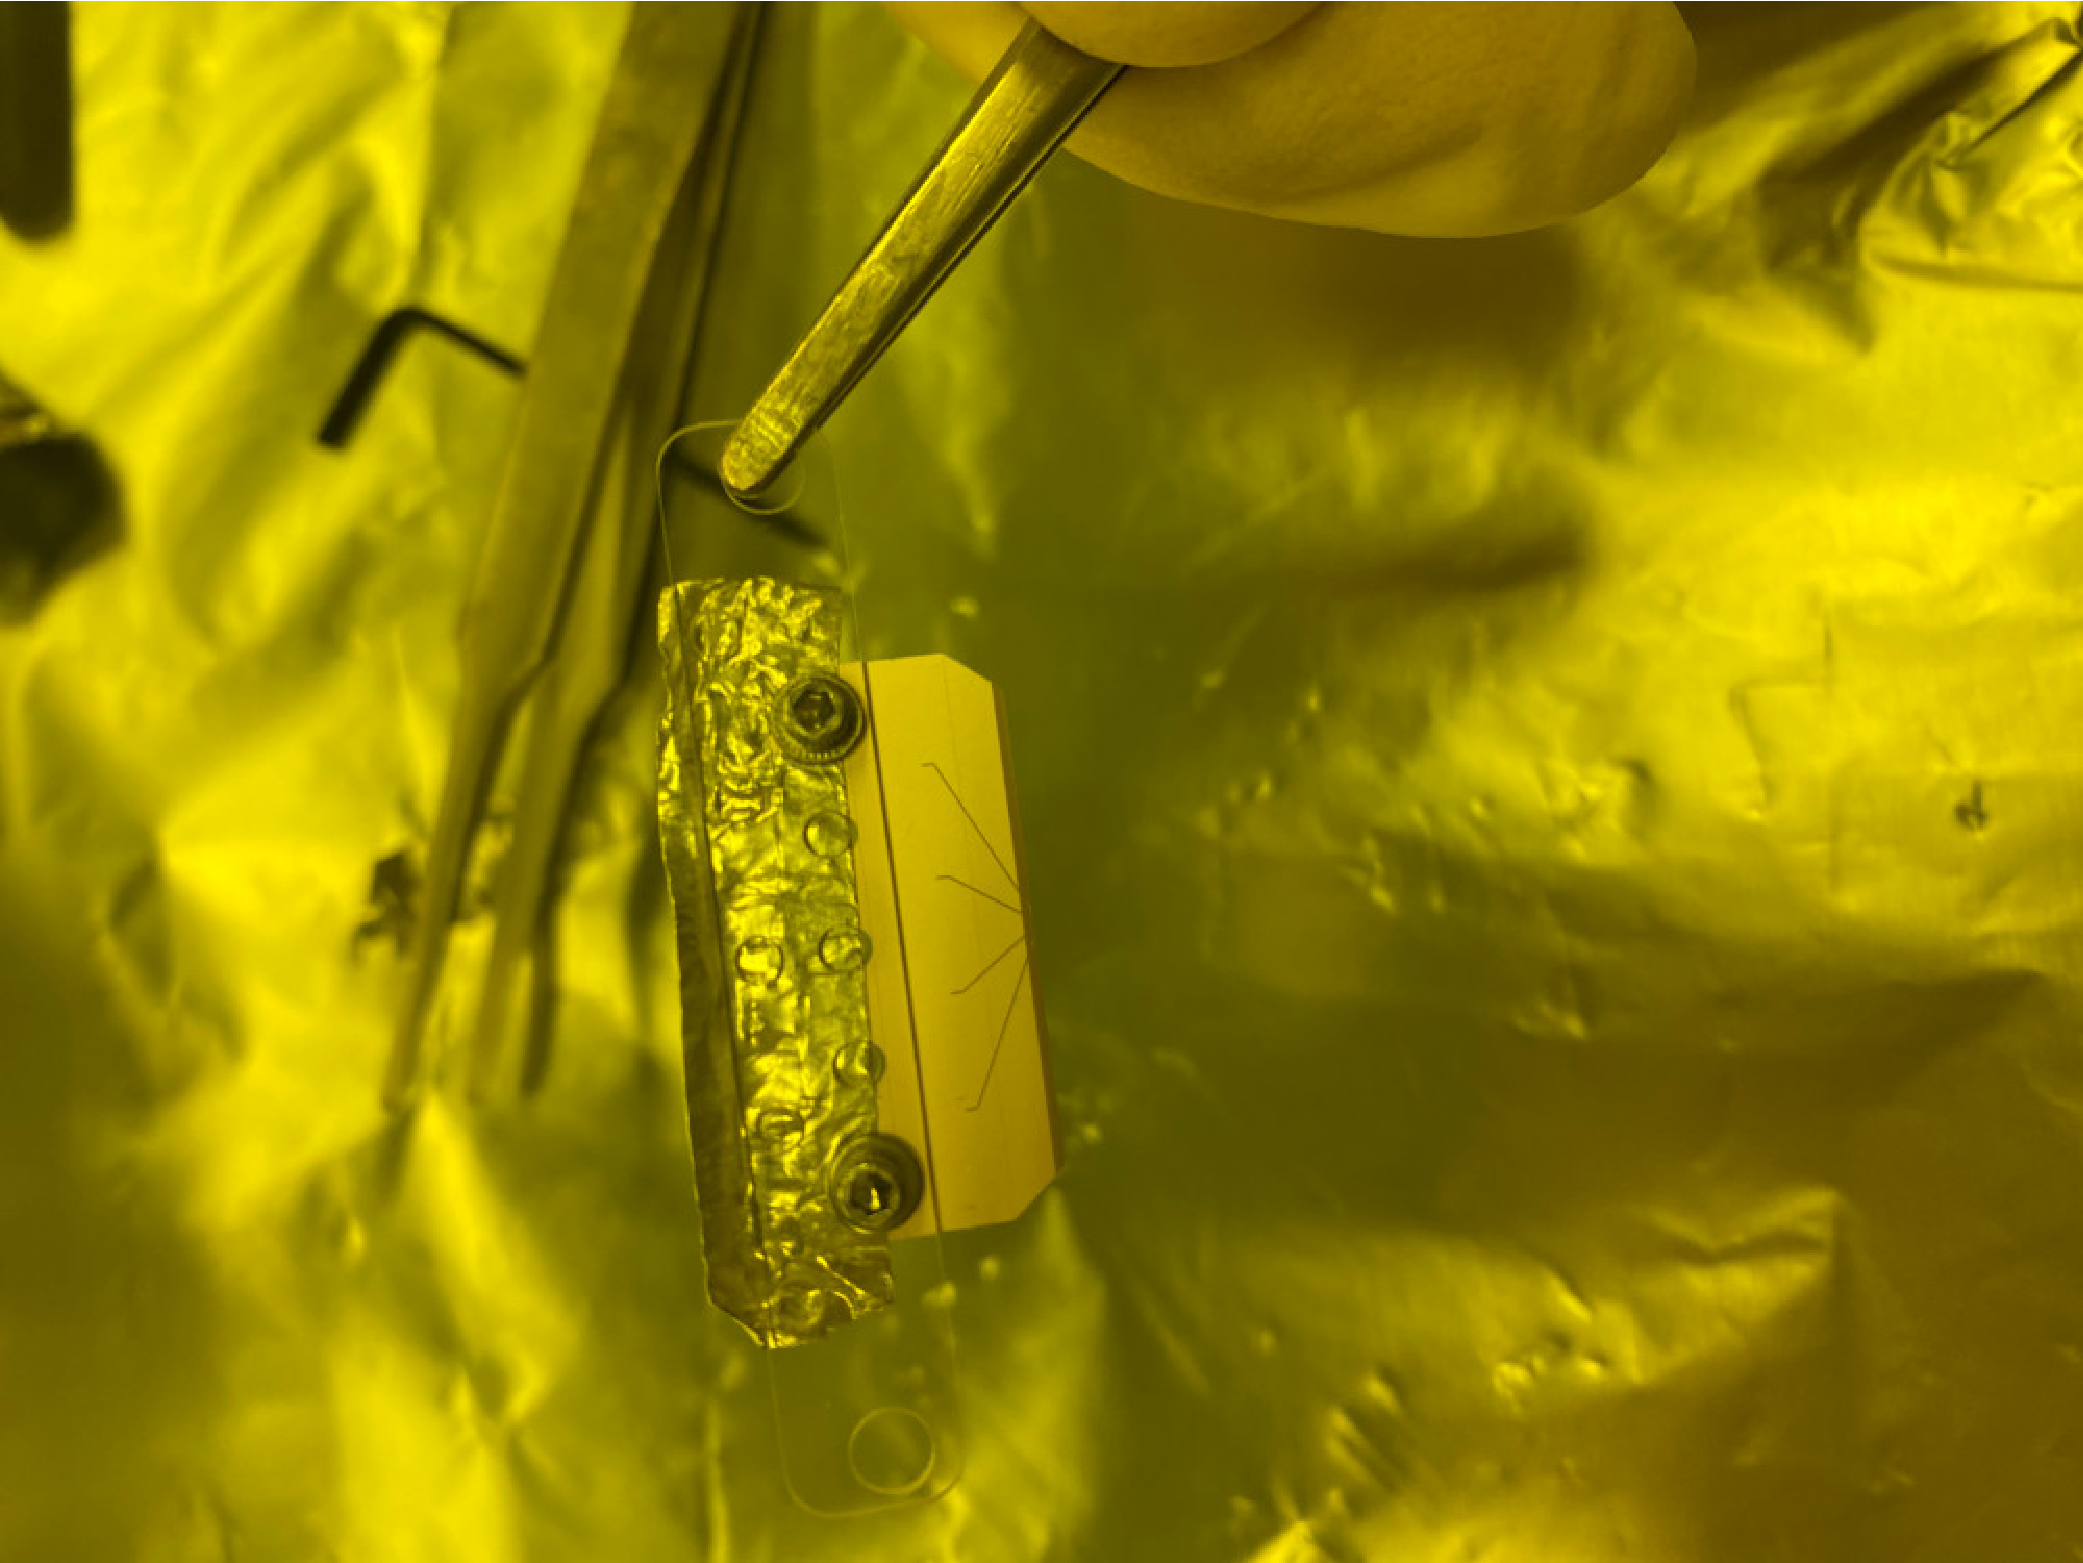
\includegraphics[width=0.4\linewidth]{fig_3_assembly_of_trap_blade.pdf}}
    \subcaptionbox{Assembly of the PCB and the gold ribbon.}
    {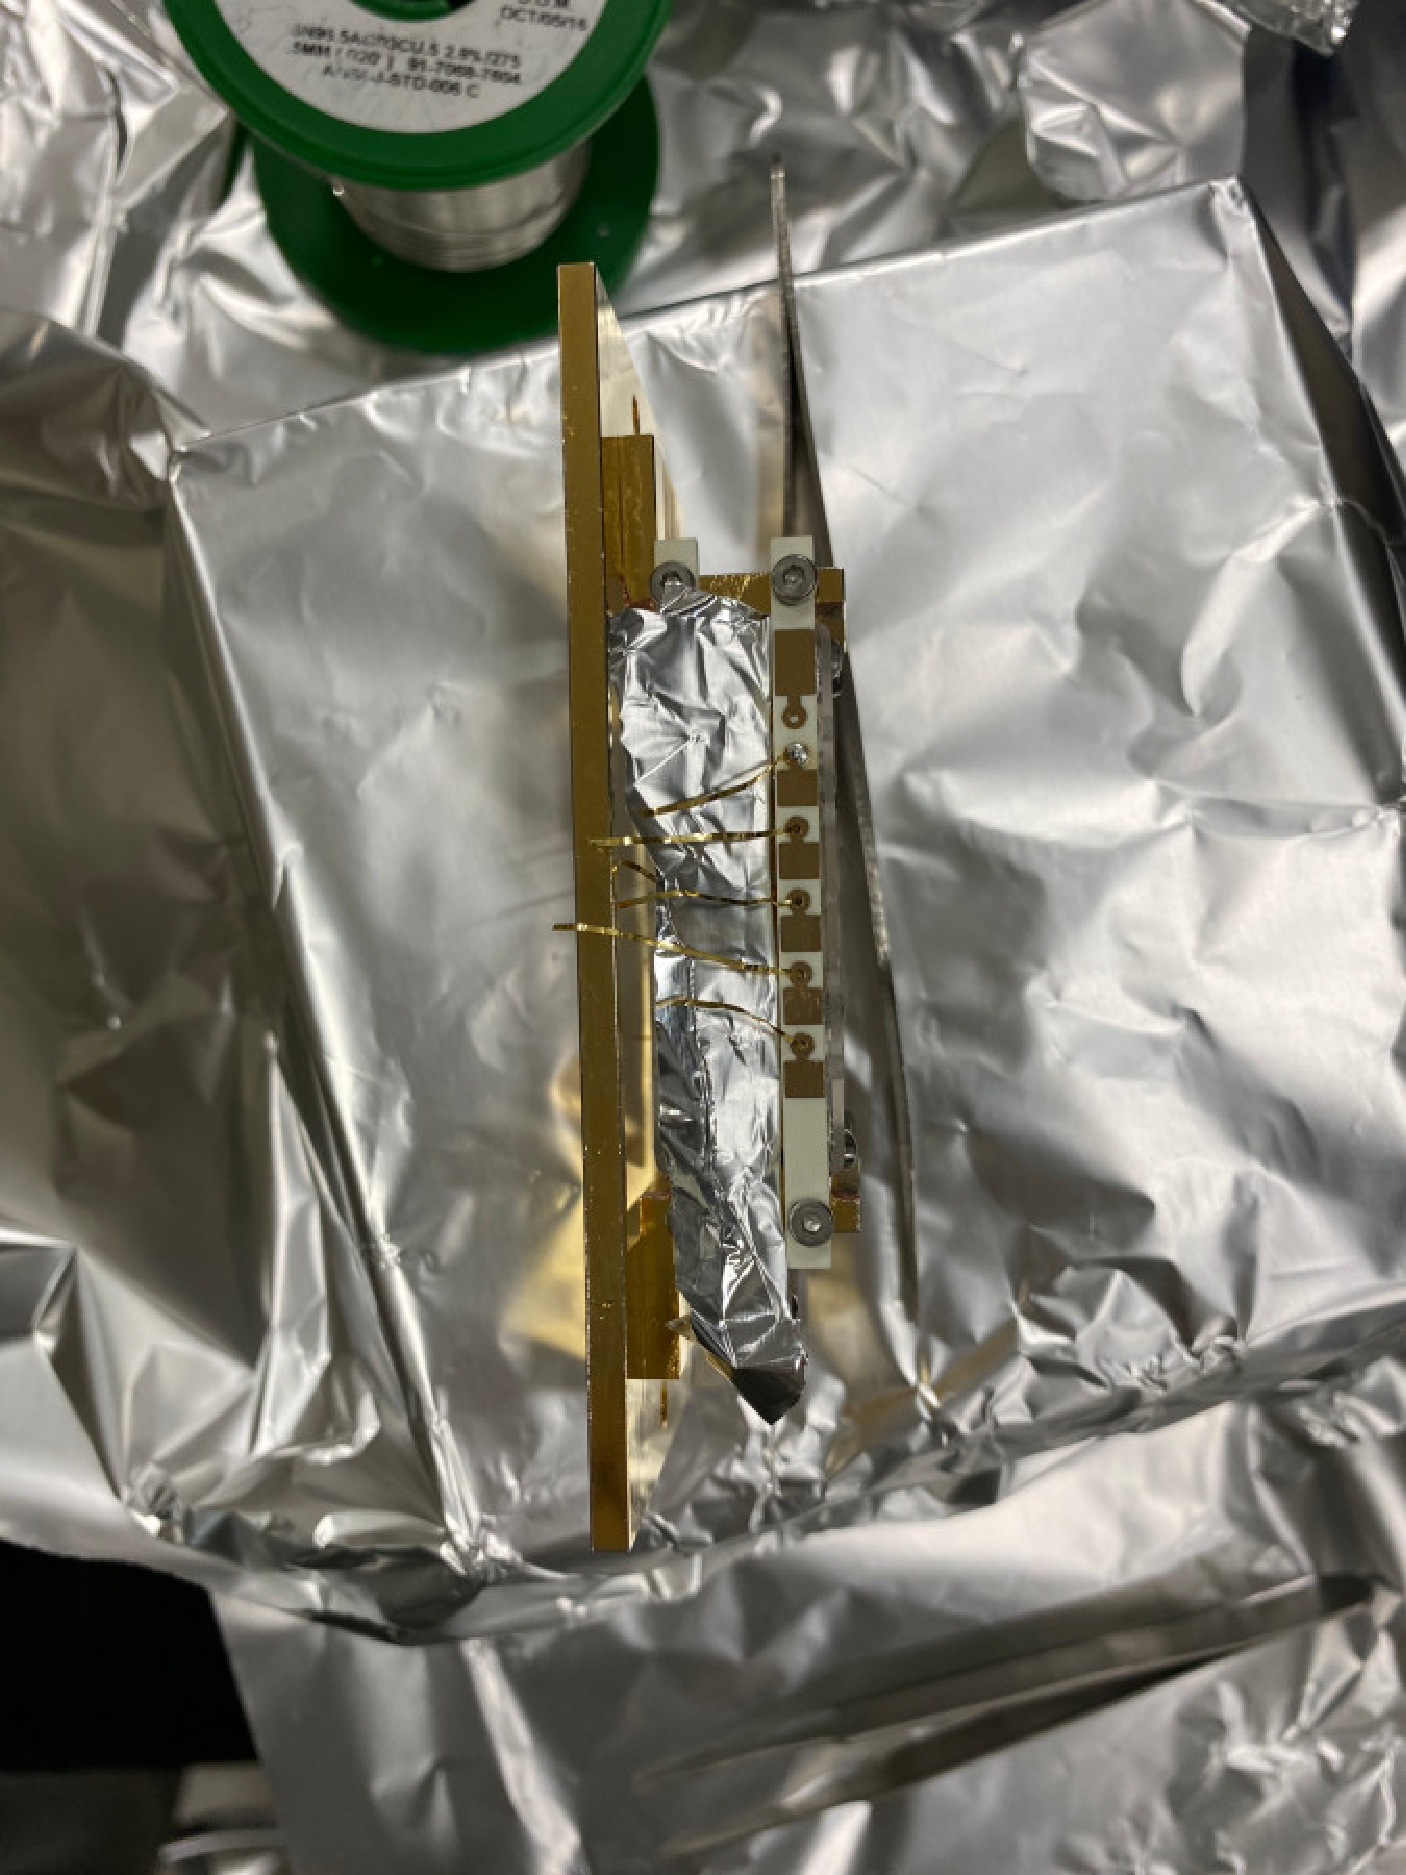
\includegraphics[width=0.4\linewidth]{fig_3_assembly_of_trap_pcb.pdf}}
    \caption{Assembly of the blade trap.}
\end{figure}

\begin{table}
    \centering
    \caption{Assembly procedures of the blade trap.}
    \begin{tabular}{p{0.2\linewidth}p{0.7\linewidth}}
        \toprule
        Procedure    & Content                                                                                                                                                                                                                                                                     \\

        \midrule
        Checking     & Soak the blades in acetone bath for 30 minutes and soak the blades in ethanol bath for 5 minutes, as the blades are very important and fragile.                                                                                                                             \\
                     & Process the DC 820pF capacitors, soak them in acetone bath for 5 minutes and soak them in ethanol bath for 1 minute.                                                                                                                                                        \\
                     & Lean the blades against the beaker, otherwise it is not easy to be taken out when it sinks.                                                                                                                                                                                 \\
                     & The position of the DC capacitor is chosen to allow for clearance for the screws, as well as for the gold ribbon.                                                                                                                                                           \\
                     & The blades can be soaked in ethanol bath when not in use.                                                                                                                                                                                                                   \\
        Spot welding & Process the gold ribbon by sonicating it with acetone for 30 minutes and with ethanol for 5 minutes.                                                                                                                                                                        \\
                     & Cover the welding machine with aluminium foil before placing the blades to prevent them from scratching.                                                                                                                                                                    \\
        Preparation  & Prepare hlders, PCBs, sapphire chips, indium foil, M2 and M1.5 screw sets and spanners.                                                                                                                                                                                     \\
                     & Make indium foil soaked in acetone bath for 30 minutes and in ethanol bath for 5 minutes and sonicate the rest with acetone for 30 minutes and with ethanol for 5 minutes.                                                                                                  \\
        Assembly     & Apply indium foil to the sapphire piece, with the front of the indium foil flush with the top of the round hole to prevent short-circuiting the blade.                                                                                                                      \\
                     & Hold the blade parallel to the sapphire piece, remove the excess indium foil and fold the top of the gold ribbon                                                                                                                                                            \\
                     & Attach indium foil to the holder, then fix the sapphire piece to it, fix the PCB board to the side of the holder and pass the gold ribbon through the air, leave a certain length of gold ribbon to prevent it from melting when soldering and donnot block the light path. \\
        \bottomrule
    \end{tabular}
\end{table}

The blade trap consists of four blade-shaped electrodes, one pair of DC electrodes and one pair of RF electrodes. The blade is processed by laser cutting the ceramic substrate and then plating the surface with a gold layer. The electrodes are machined with a certain amount of error and defects on the surface of the electrode closest to the ion. They will produce a high level of electrical noise, which can be reduced by improving the process. We have machined a sapphire adapter plate and mounted the blade on the sapphire adapter plate and then mounted the sapphire adapter plate on an oxygen-free copper holder. We designed this adapter to avoid a short circuit between the blade and the ground (the blade holder). In order to increase the thermal conductivity, we need to cover these contact surfaces with indium foil. For the fixing of the components, we used stainless steel screws and used resilient pads on each screw. This is to prevent the screws from loosening during the cooling down process and to prevent the blade from being crushed by excessive torque when tightening the screws. Once installed, we had to fine-tune the position of the sapphire adapter under the microscope to keep the assembly error small enough. This operation makes use of the fact that the diameter of the through-hole is slightly larger than the diameter of the screw. Since the assembly is done by hand, this part of the assembly error is unavoidable.

The connection of the blade electrodes is mainly done by means of gold ribbon (AMETEK) and Kapton insulated wire (Accu-Glass Products). When selecting materials we need to be aware of ultra-high vacuum and cryogenic compatibility. Some of the circuit connections are made prior to assembly and the rest is done afterwards. Before assembling the blade, a 820 pF capacitor is fixed with silver epoxy between each DC electrode and ground on the two DC blades. The purpose of this capacitor is to create a low impedance between the DC electrodes and ground, reducing the voltage splitting of the RF signal on the DC electrodes. The gold ribbon is connected to the electrodes with the spot welder at one end and to the pads of the PCB with solder at the other. We will later connect the pads to the corresponding connections with Kapton insulated wire, where the DC electrode wires are connected to the corresponding wires from the DC feedthrough through the heat sink twice and the two RF electrode wires are connected to the two wires at the output of the helical resonator.



\section{Yb oven}

In order to generate the atomic beams of ytterbium, we built two separate ovens from two stainless steel tubes, but integrated into a single feedthrough and both able to be used to load ions. The ${ }^{171} \mathrm{Yb}$ oven has an abundance of 90\% and the ${ }^{174} \mathrm{Yb}$ oven has an abundance of 98\%. As the Yb source is in block form, we need to cut it into small pieces and insert it into the stainless steel tube.

\begin{figure}
    \centering
    \subcaptionbox{Put all the components together.}
    {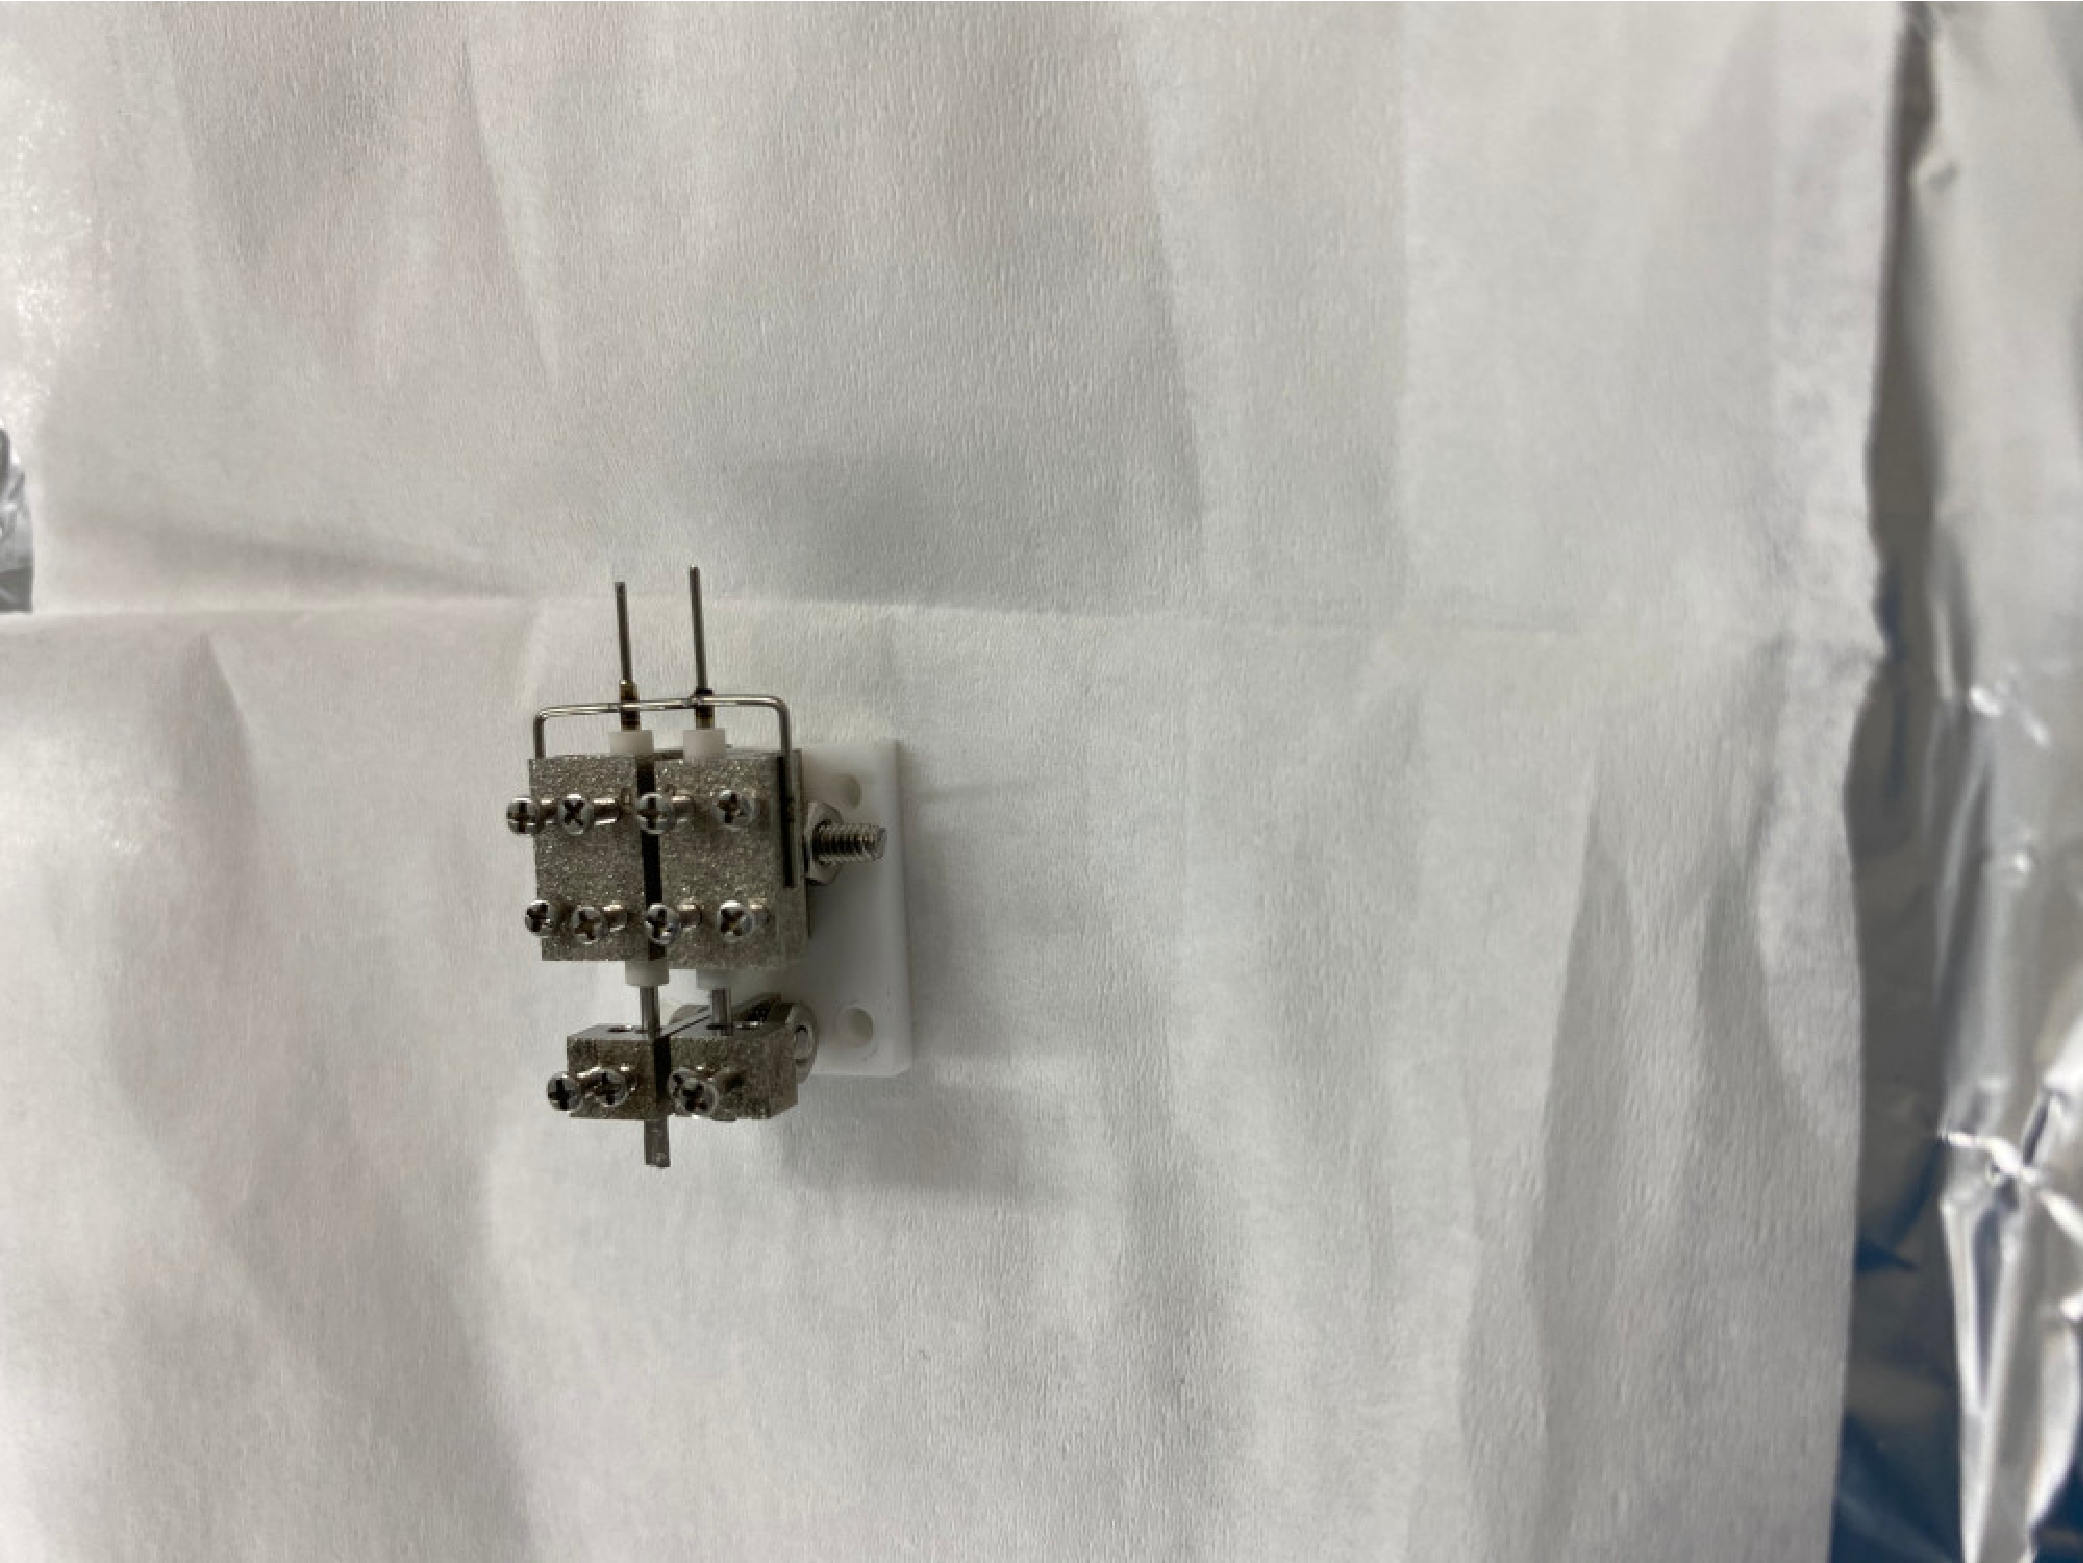
\includegraphics[width=0.4\linewidth]{fig_3_assembly_of_oven_1.pdf}}
    \subcaptionbox{Connect to feedthrough.}
    {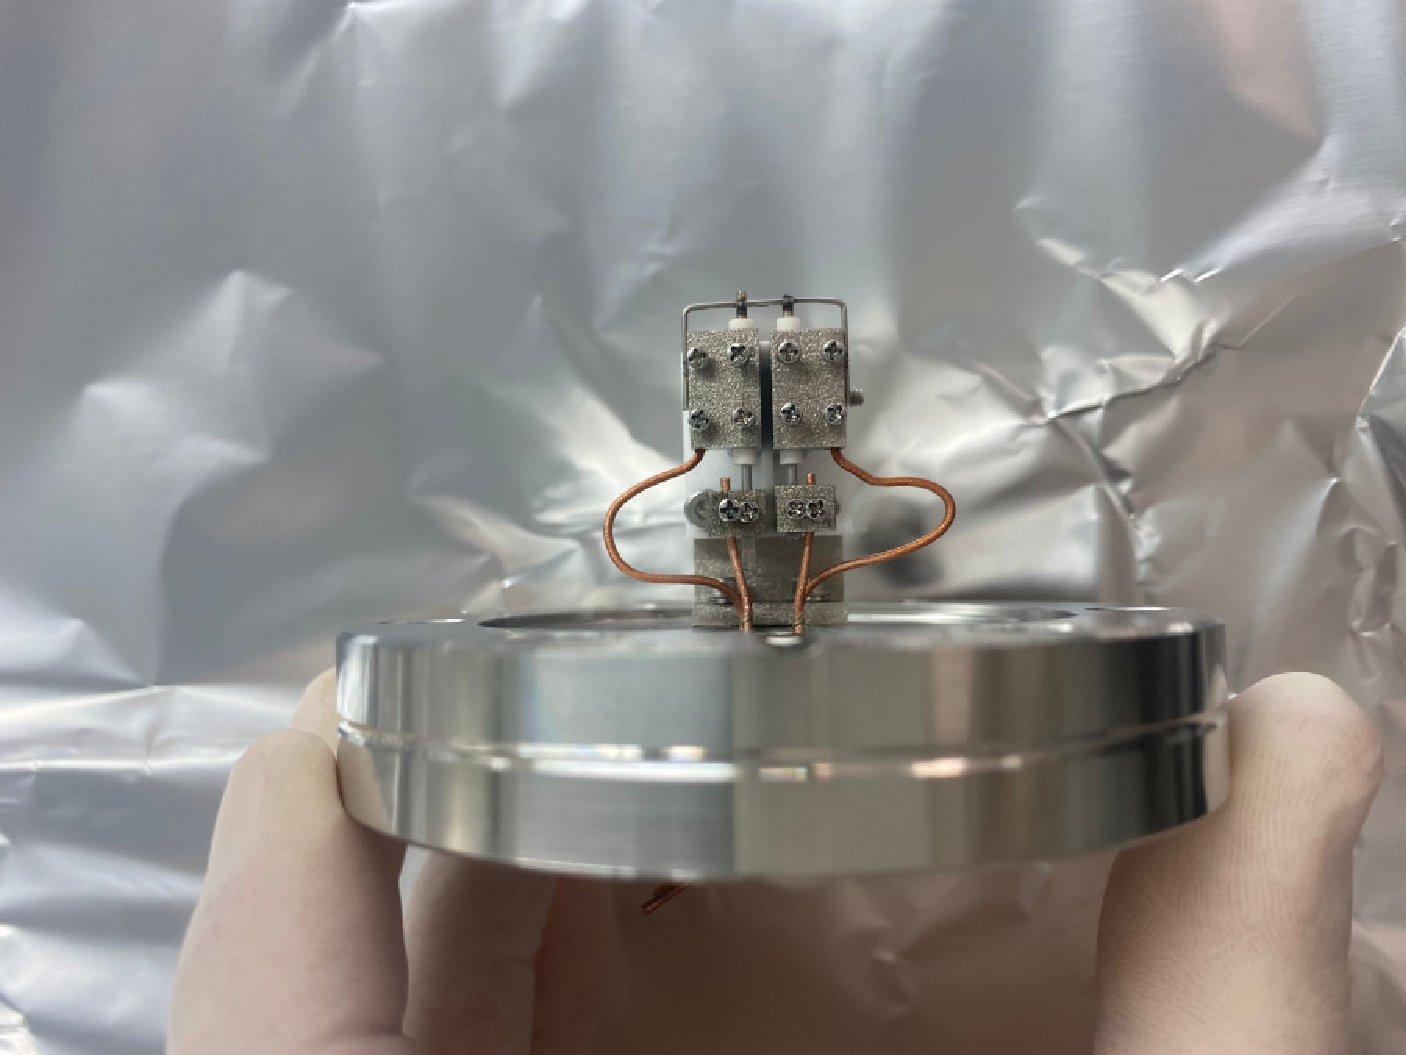
\includegraphics[width=0.4\linewidth]{fig_3_assembly_of_oven_2.pdf}}
    \caption{Assembly of the ytterbium oven.}
\end{figure}

In order to achieve UHV compatibility, we chose to use copper, stainless steel and Macor when machining the parts of the oven. Before assembly and testing, we cleaned all the parts inside the ultrasound machine using acetone and ethanol as solvents. All the parts were assembled according to the drawings and the copper wires on the feedthrough were attached to the stainless steel base, which was all screwed in place. We then used a spot welder and welded the stainless steel tube to the stainless steel wire, and the stainless steel wire to the stainless steel base, respectively. As the stainless steel tube has the smallest cross-sectional area, the highest resistance in the whole circuit is at the stainless steel tube, about 0.5 $\Omega$, so the temperature is highest here too. I would recommend having some extra spare parts and testing the parameters of the spot welder in advance, as the stainless steel tube can easily break under unsuitable parameters. Finally the two Yb sources are filled into the corresponding stainless steel tubes.

\begin{figure}
    \centering
    \subcaptionbox{Testing in a vacuum.}
    {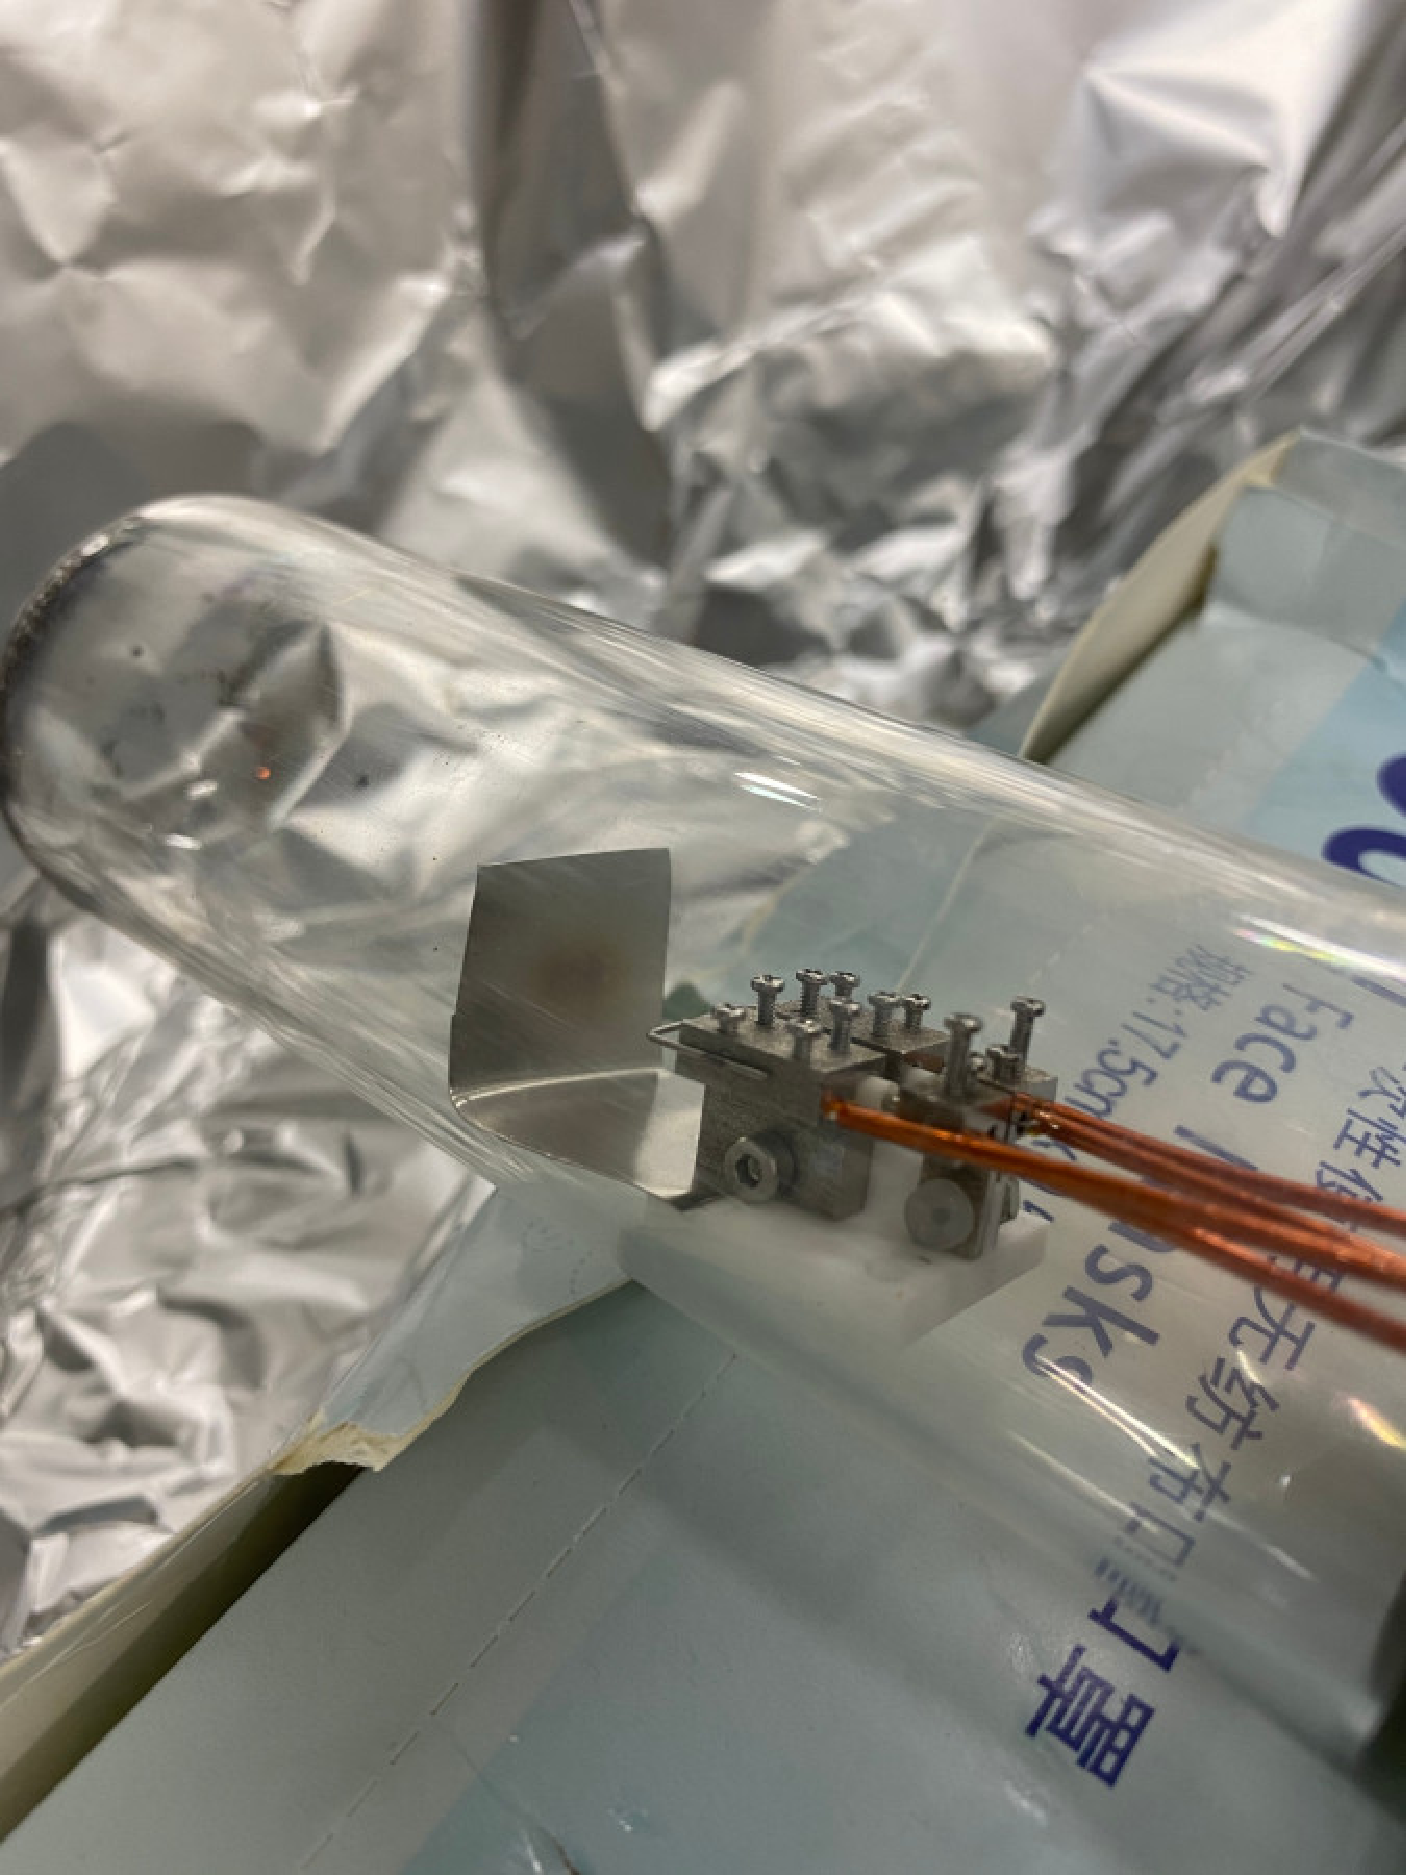
\includegraphics[width=0.3\linewidth]{fig_3_test_oven_1.pdf}}
    \subcaptionbox{Observation in the atmosphere.}
    {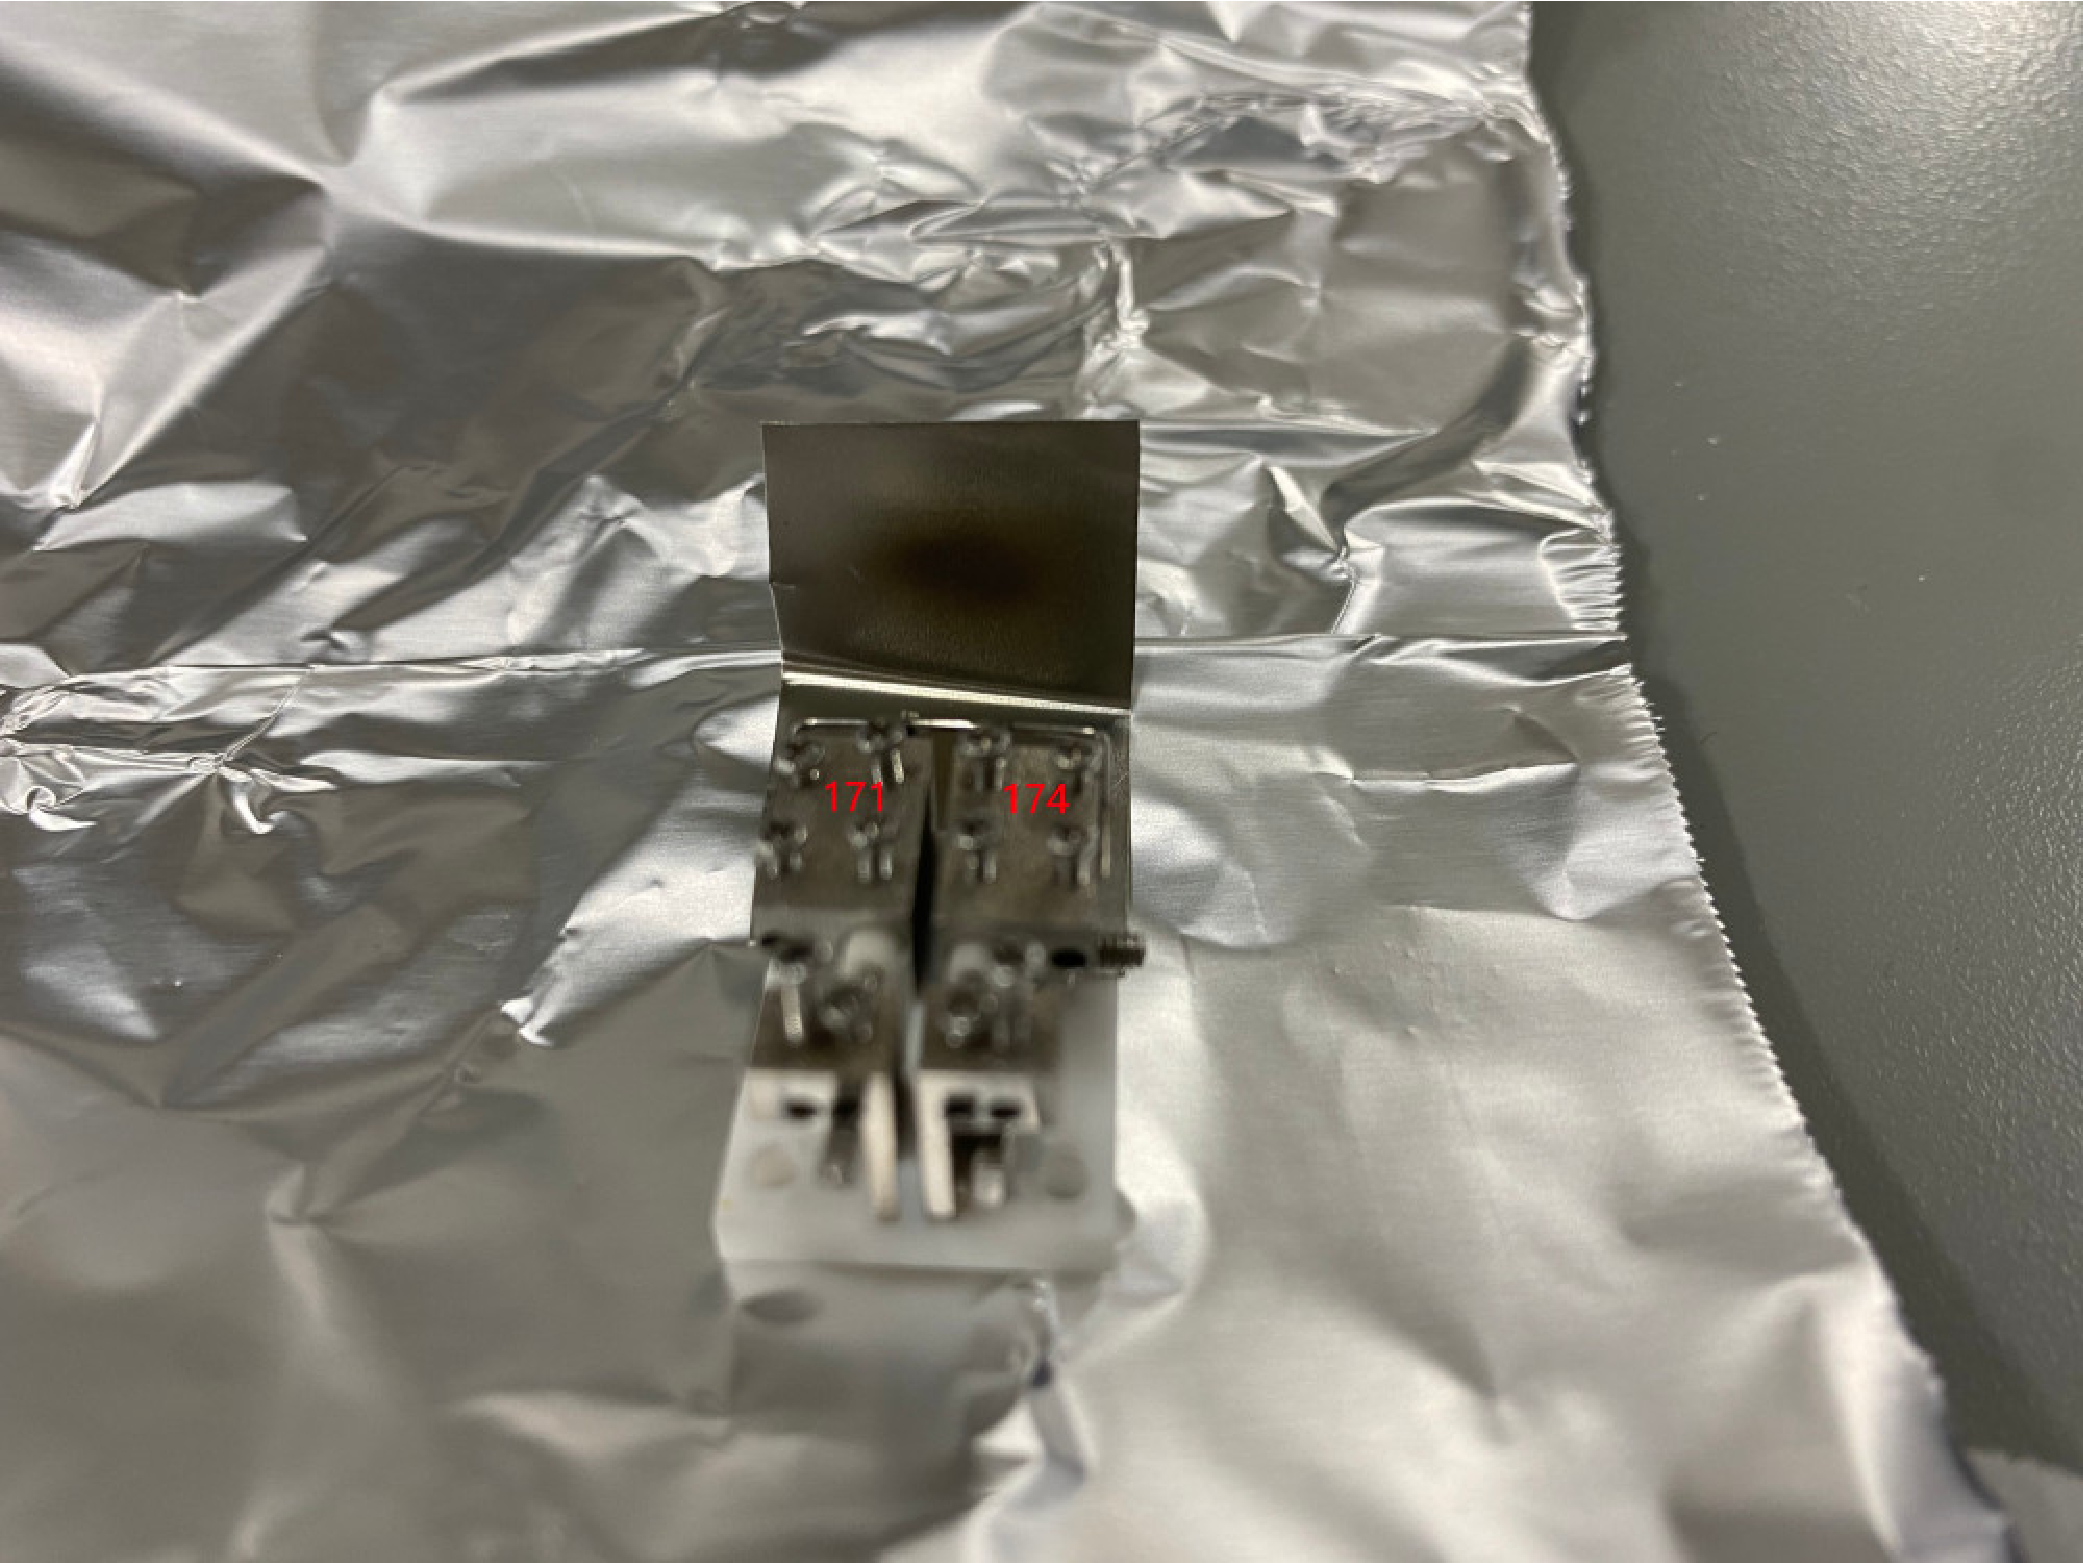
\includegraphics[width=0.5\linewidth]{fig_3_test_oven_2.pdf}}
    \caption{Testing of the Yb oven.}
\end{figure}

Each oven is mounted in such a way that the outgoing atomic beam is directed towards the trapping area. The oven feedthrough replaces an 1 inch window in the axial direction of the trap. the glass in the corresponding position of the 40 K shield and 4 K shield is also replaced with a round aluminium plate, the centre of which is a square hole with a 5mm side to pass through the Yb flux. As the cryostat has assembly errors, I would recommend preparing round aluminium plates with different opening positions in advance. Ultimately we need to be able to see the trap through the opposite window, with the square hole and the oven in the same line.

\begin{table}
    \centering
    \caption{Parameter variation during testing the Yb oven.}
    \begin{tabular}{llll}
        \toprule
        Oven                            & Initial vacuum              & Ending vacuum               & Threshold current \\

        \midrule
        ${ }^{171} \mathrm{Yb}$ (Left)  & $4.0 \times {10}^{-6}$ mbar & $8.6 \times {10}^{-6}$ mbar & 4.2 A             \\
        ${ }^{174} \mathrm{Yb}$ (Right) & $2.3 \times {10}^{-6}$ mbar & $6.5 \times {10}^{-6}$ mbar & 3.9 A             \\
        \bottomrule
    \end{tabular}
\end{table}


In the process of loading ions, when this stainless steel tube is heated resistively by an electric current, a spray of atomic Yb is produced. The temperature reached depends on the current and the time of operation. If either of these two factors is too high or too long, this can lead to rapid evaporation of the Yb and thus the formation of a spray dense enough to cover its surface (e.g. ion trap electrodes or vacuum windows). To prevent this, each oven is tested in advance. A stainless steel sheet is placed in front of the oven and then the oven is placed in a transparent vacuum chamber and the vacuum is reduced to approximately $4 \times {10}^{-6}$ mbar using a turbo-molecular pump, so that a test system can be set up. We tested each oven in turn, starting at 0 A and increasing the current by 0.1 A every 10 seconds, observing the change in vacuum level and the colour of the stainless steel sheet. We can observe both the darkening of the stainless steel sheet and the rapid rise in pressure, at which point the current value is the threshold current for the corresponding oven. ${ }^{171} \mathrm{Yb}$ oven has a threshold current of 4.2 A and ${ }^{174} \mathrm{Yb}$ oven has a threshold current of 3.9 A, but the current values we use in practice will be lower than this threshold. The exact values need to be measured in the corresponding experiments. The exact values need to be measured in corresponding experiments, such as observing the fluorescence of Yb atoms and loading Yb ion.



\section{Optical and imaging system}

\begin{figure}
    \centering
    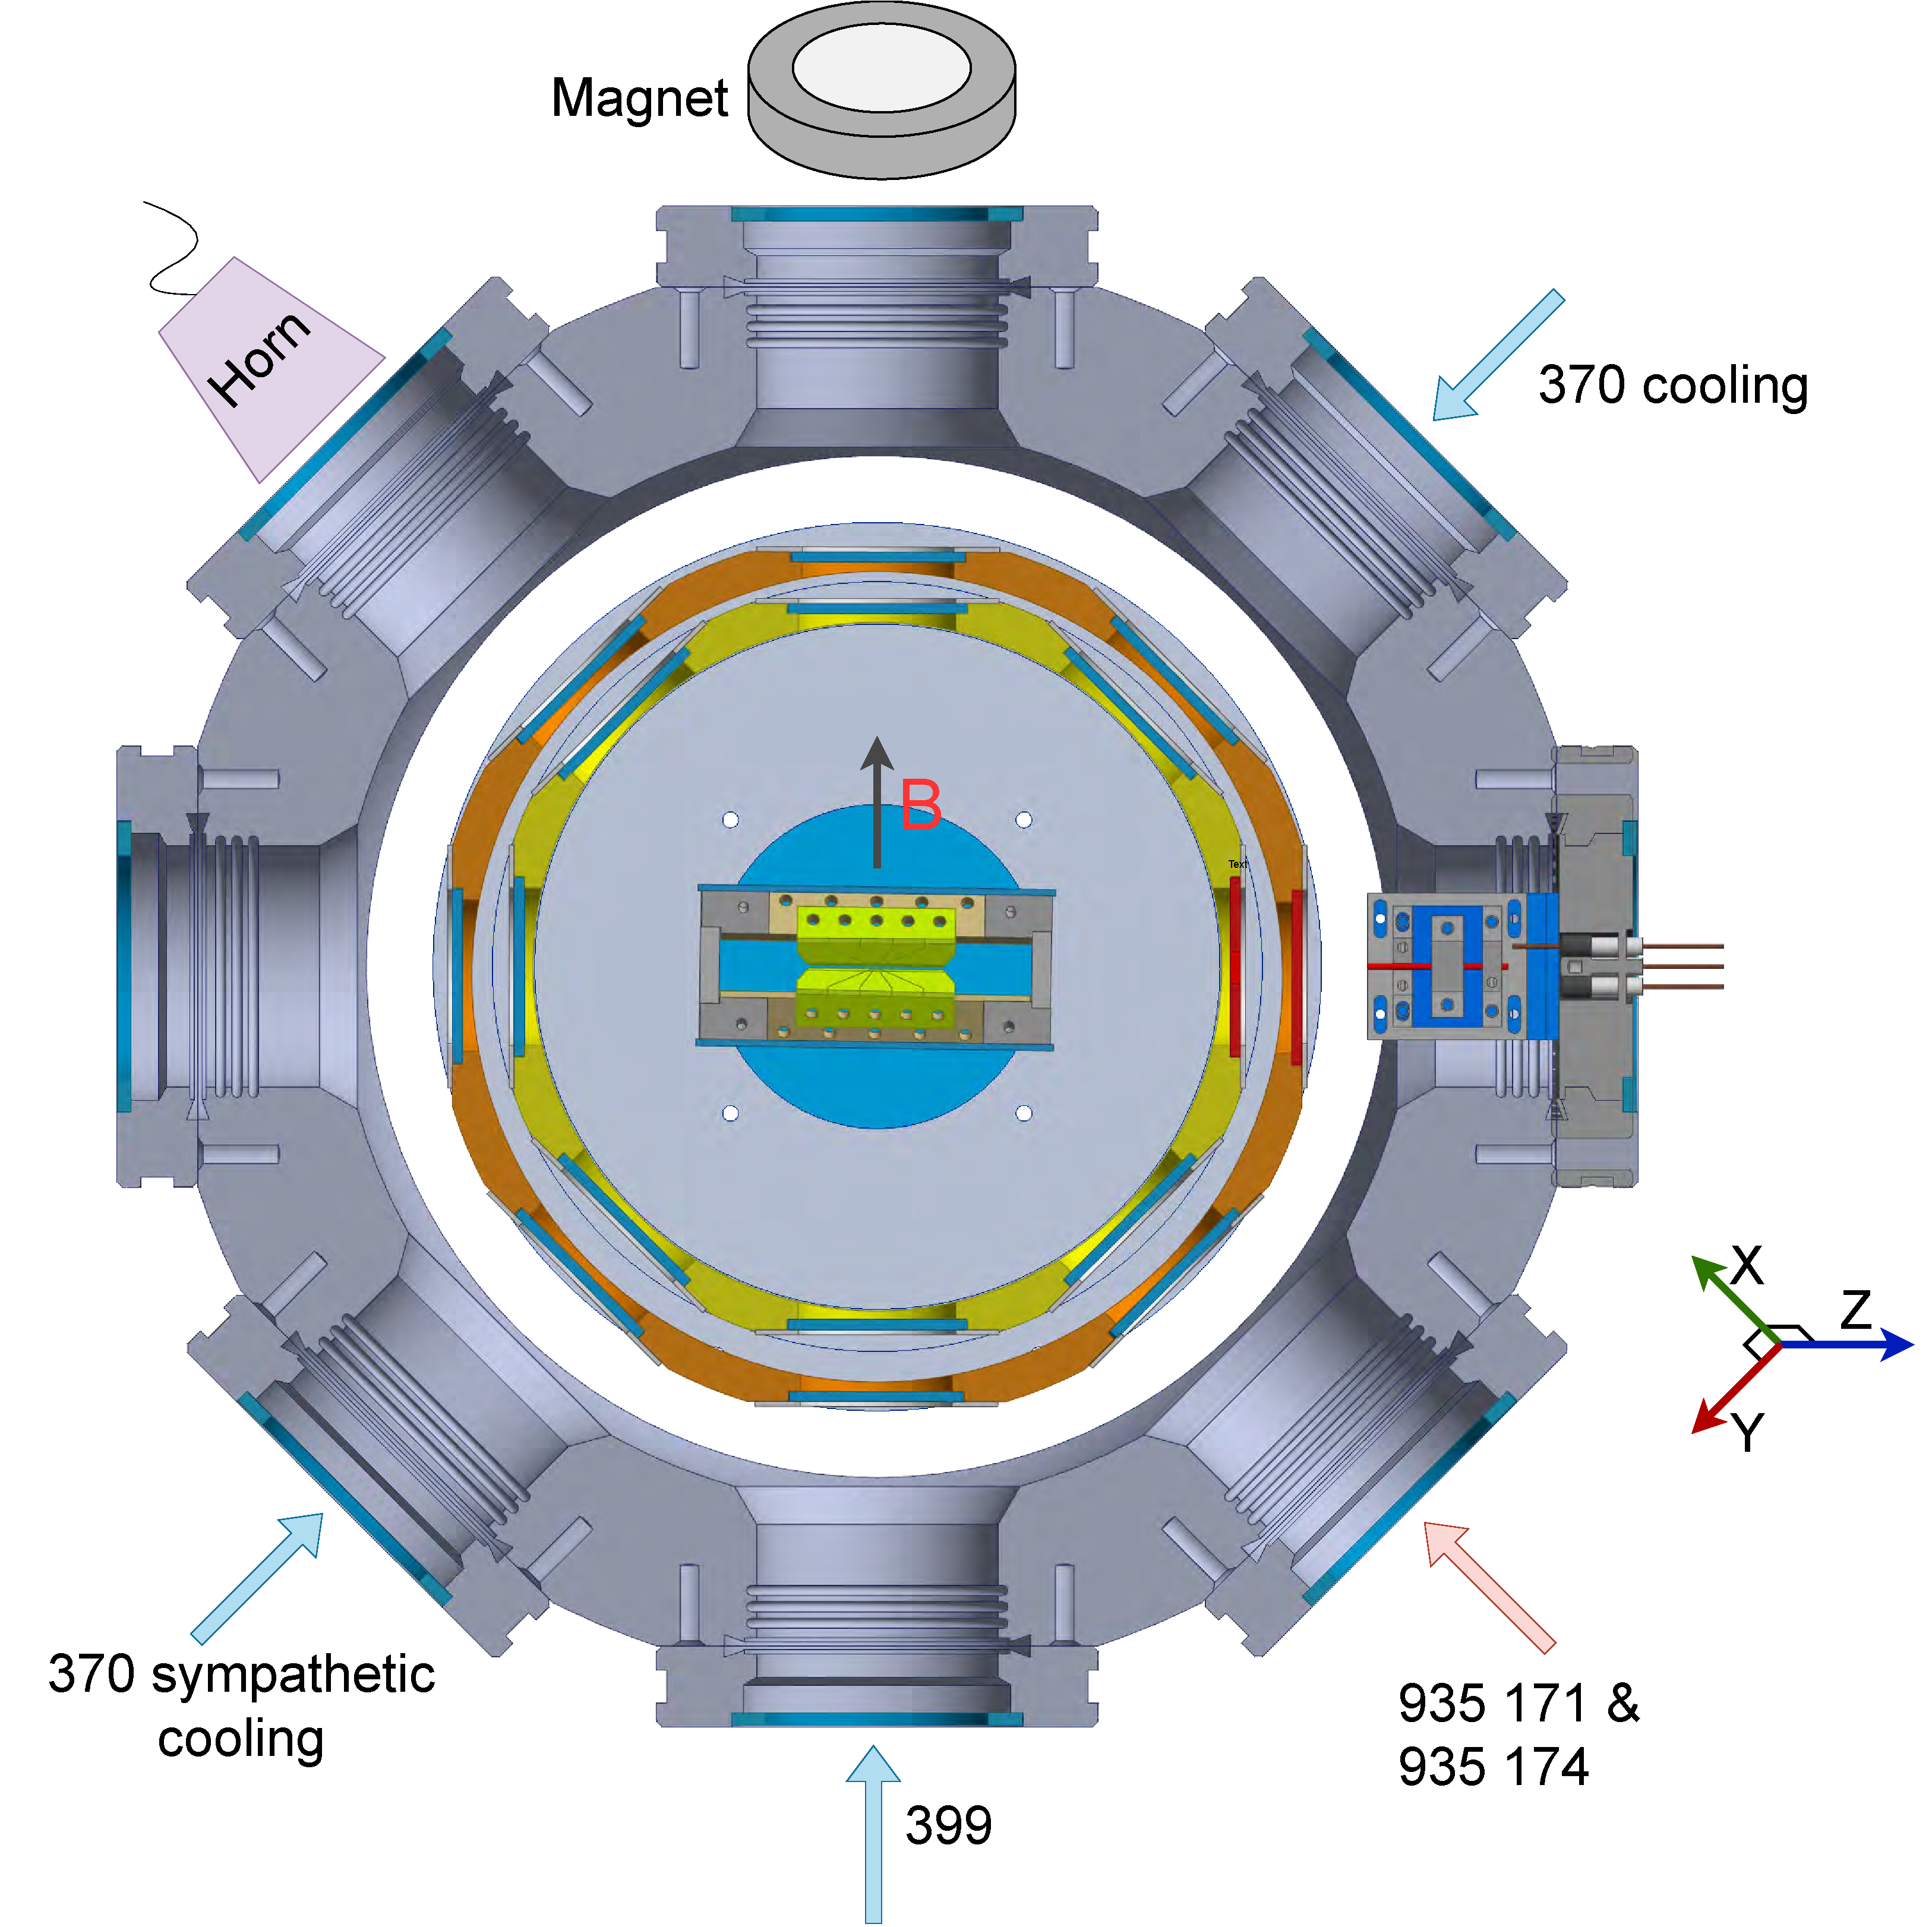
\includegraphics[width=0.7\linewidth]{fig_3_optical_layout_of_ion_trap_and_vacuum_chamber.pdf}
    \caption{Optical layout of the ion trap and the vacuum chamber.}
\end{figure}

Whether trapping ions or manipulating them, we need lasers. In our laboratory, tunable diode lasers (Toptica DL pro HP) are used widely, mainly because these products are very well mature. For ion trap systems, a stable light source is very important. Experimentally, we need these lasers to be switched on and off quickly, typically in a few hundred nanoseconds. It is also necessary that these lasers can be stabilised over long periods of time and that these laser controllers have stable software systems. Laser stabilisation covers mode, frequency, power and polarisation. Typical laser stabilisation lasts from a few hours to a day, including laser frequency locking. This is sufficient for our trapped ion experiments, but longer stabilisation times are preferable. In the experiments, these stable lasers are used for: ion loading, Doppler cooling, optical pumping, state detection, repumping and sympathetic cooling. In addition to the laser light path into the cavity, I also built an imaging system to collect the fluorescence emitted by the ions, enabling real-time observation and state detection of the ions.

\subsection{Laser sources and power allocation}

The light sources in the laboratory are placed on several separate optical tables. Since the principles of the optical path setup are similar, we can present the light sources and power allocation in a common way, as shown in Fig~\ref{fig:fig_3_optical_path_diode_laser}. The cryogenic trap platform requires a 370 nm laser (L1), a 399 nm laser (L2) and two 935 nm lasers (L3, L4). The two 935 nm lasers are shared with other ion trap platforms in the lab, one for trapping ${ }^{171} \mathrm{Yb}^{+}$ ions and the other for trapping ${ }^{174} \mathrm{Yb}^{+}$ ions. The 399 nm laser is used for loading ions. Depending on the type of ion to be loaded, ${ }^{171} \mathrm{Yb}^{+}$ or ${ }^{174} \mathrm{Yb}^{+}$, we can change the wavelength of the 399 nm laser. This 399 nm laser is also shared with other trapped ion platforms in the lab and only one 399 nm laser is needed. Since loading ions is not very frequent and most of the time we need to load ${ }^{171} \mathrm{Yb}^{+}$ ions, and modifying the wavelength of the 399 nm laser will not affect the stable trapping of the loaded ions.

\begin{figure}
    \centering
    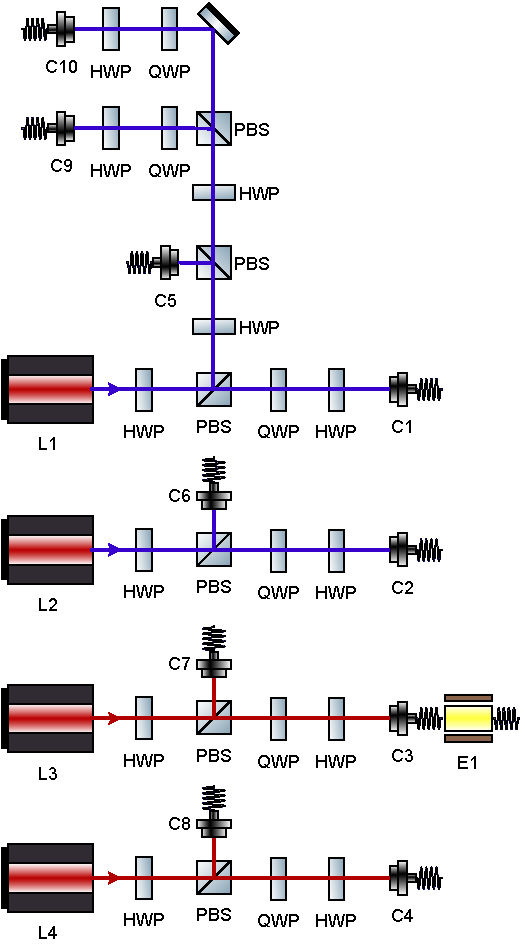
\includegraphics[width=0.4\linewidth]{fig_3_optical_path_diode_laser.pdf}
    \caption{Optical path of laser power allocation.}
    \label{fig:fig_3_optical_path_diode_laser}
\end{figure}

The output power of a semiconductor laser is approximately 10 mW, depending on the wavelength and model, the laser output power may vary a little. The output power of the 370 nm laser (L1) is 13 mW,
other lasers have similar output power.

As the nominal light output from the laser is linearly polarised, a power attenuation unit was formed using a half-wave plate (HWP) and polarization beam splitter (PBS) to split the laser output into two parts, which are separately coupled into the fibre. Each fibre will act as the light source for the next stage of the optical path, thus making the optical path a modular one. Each laser has one optical fibre connected to the wavemeter (C5, C6, C7, C8). Because polarisation stabilisation is not required, a single-mode fibre is used, with a typical power of approximately 50 µW. The other fibres are the light sources for the rear optical paths (C1, C2, C3, C4) and require high power, typically 5 mW. At the same time their polarisation needs to be stable over time and we use single-mode polarization-maintaining fibres. In order to adjust the polarisation direction to match that of the single-mode polarisation-maintaining fibre, we use a polarisation adjustment unit consisting of a HWP and quarter-wave plate (QWP). We need to maximize the efficiency of the fiber coupling, which requires a good laser output mode and good mode matching, which can be done with a lens pair, I don't show this in the diagram.

\begin{table}
    \centering
    \caption{Wavelengths of lasers in the laboratory corresponding to loading different isotopes.}
    \begin{tabular}{llll}
        \toprule
        Isotope                     & 370 Laser (nm) & 399 Laser (nm) & 935 Laser (nm) \\
        \midrule
        ${ }^{171} \mathrm{Yb}^{+}$ & 369.526334     & 398.911150     & 935.188        \\
        ${ }^{174} \mathrm{Yb}^{+}$ & 369.525228     & 398.911570     & 935.180        \\
        \bottomrule
    \end{tabular}
\end{table}

The 370 nm laser also has two splits: one (C9) is connected to the optical cavity for narrow linewidth frequency locking of the laser, and the other (C10) is set aside. ${ }^{171} \mathrm{Yb}^{+}$ repumping beam requires 3.0695 GHz sidebands, so the 935 nm laser (L3) has a fibre EOM (E1) in the rear optical path.

\subsection{Laser frequency stabilization}

\begin{figure}
    \centering
    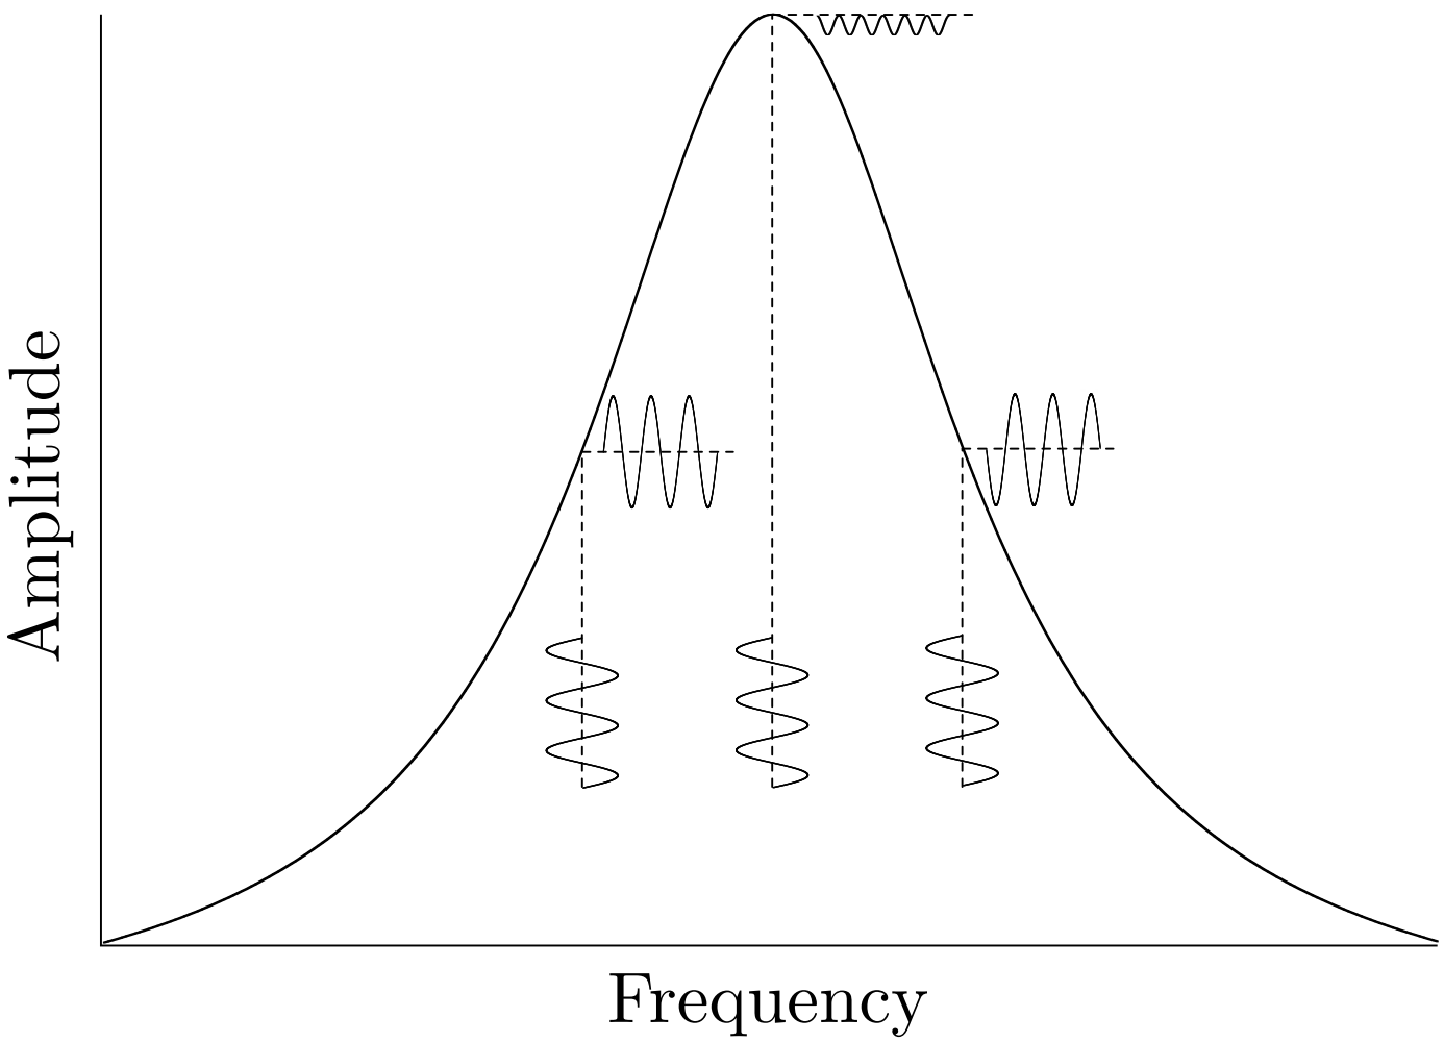
\includegraphics[width=0.4\linewidth]{fig_3_principle_of_frequency_modulation_for_optical_cavity.pdf}
    \caption{Illustration of simple frequency modulation for optical cavity.}
\end{figure}

The target linewidth of the laser frequency locking determines the laser frequency locking scheme \cite{RN137,RN151,RN76}. In my experiments there is no need for ultra-narrow linewidth laser locking, so the laser locking scheme is relatively simple and I have mainly optimised the automatic control of the frequency locking process. The measurement and locking of the laser frequency can be achieved with a wavelength meter, which has a relatively low bandwidth of about 10 Hz because the sum of the measurement time of the multi-channel wavelength meter and the computer readout time is about 100 ms, as shown in Fig~\ref{fig:fig_3_optical_path_wave_meter}. The standard deviation of the output frequency of the laser locked with this scheme is about 1 MHz, which meets my needs with a 399 nm laser and two 935 nm lasers, or if only to trap a small amount of ions then also my requirements for a 370 nm laser \cite{RN78}. The outgoing light from the laser is transmitted by optical fibres (C5, C6, C7, C8) to the input of the wavemeter, which is programmed to read the frequency on our PC and then programmed to adjust the voltage signal from the laser controller, thus creating a closed loop that locks the laser frequency. The wavemeter's measurements are affected by the environment, mainly air pressure and temperature. Therefore this frequency locking scheme will cause the locked laser frequency to be inaccurate due to inaccurate measurements, but this error is slow and periodic over time. So for 399 nm laser and 935 nm lasers we don't take this into account. I only calibrate the 370 nm laser once in 1 hour or longer, by measuring the resonant frequency of the $\mathrm{Yb}^{+}$ ion and feeding it back to the wavemeter's lock point. It would be possible to automatically calibrate the wavemeter for measurement errors if the wavemeter had a locked reference light all the way through, such as a 780 nm laser, but we have not done this because it is not necessary. The implementation of an automatic frequency lock is necessary as it will simplify the steps of daily operation. By laboratory standards these lasers need to be switched off when they are not in use, for example every night. I will adjust the operating parameters of the laser so that the laser mode can be stabilised back to a specific frequency range for approximately 10 minutes after each switch-on operation, which requires us to find a stable operating parameter for the laser. We then only need to program to communicate with the laser and the wavemeter to achieve automatic laser control and frequency locking \cite{RN231}.

\begin{figure}
    \centering
    \subcaptionbox{Optical path of the wavelength meter.\label{fig:fig_3_optical_path_wave_meter}}
    {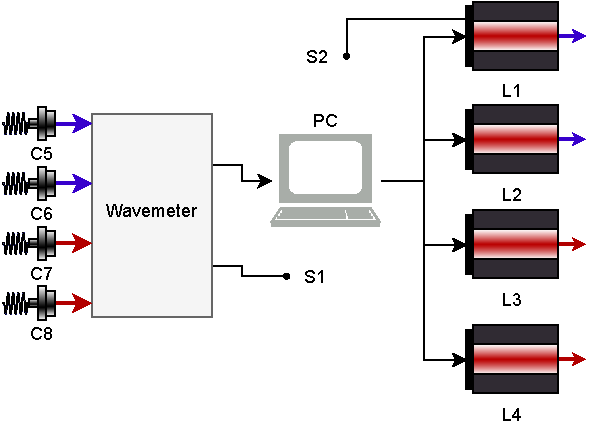
\includegraphics[width=0.4\linewidth]{fig_3_optical_path_wave_meter.pdf}}
    \subcaptionbox{Optical path of the optical cavity.\label{fig:fig_3_optical_path_370_cavity}}
    {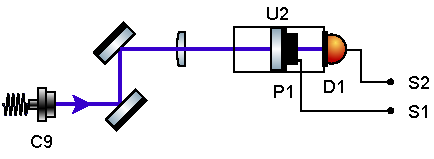
\includegraphics[width=0.4\linewidth]{fig_3_optical_path_370_cavity.pdf}}
    \caption{Optical layout of laser frequency stabilization system.}
\end{figure}

\begin{figure}
    \centering
    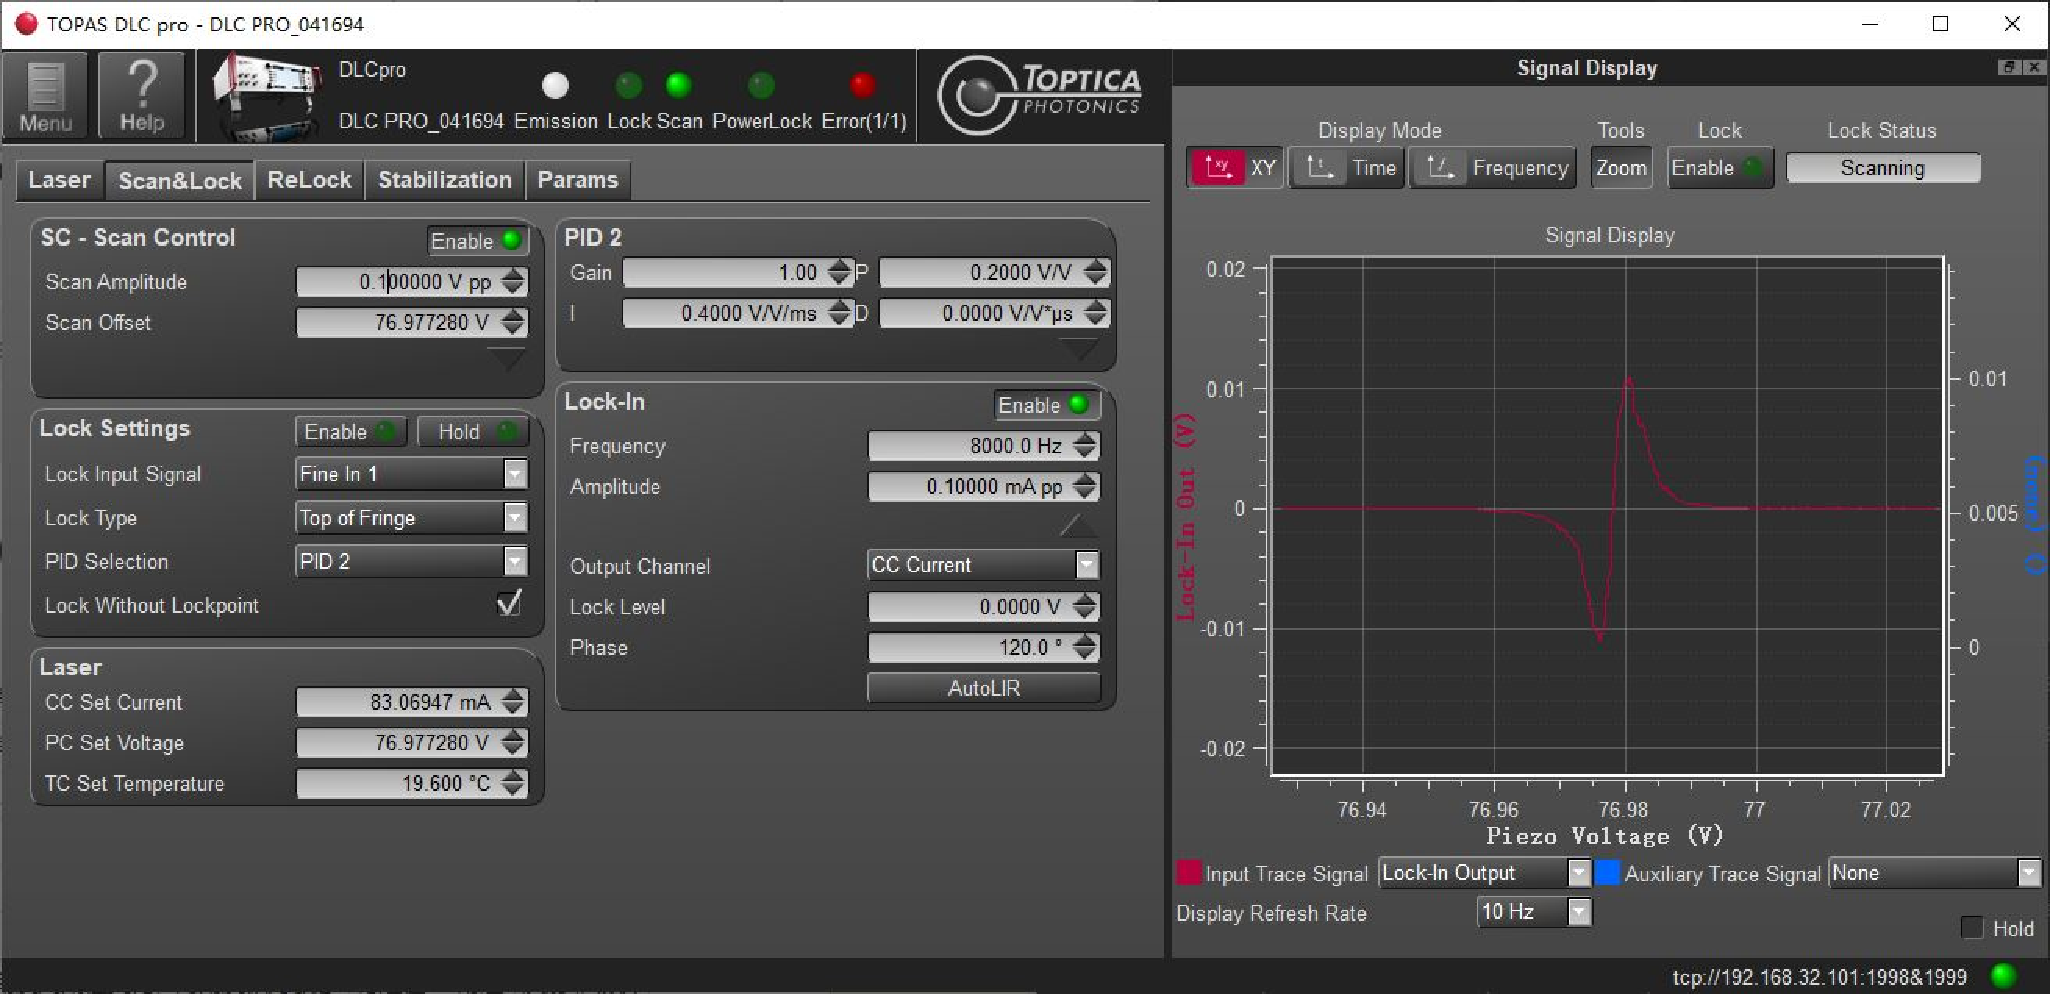
\includegraphics[width=0.8\linewidth]{fig_3_demodulated_signal.pdf}
    \caption{Demodulated signal of the optical cavity photo diode.}
\end{figure}

The results of targeting the 370 nm laser with a wavemeter are not good enough because the feedback speed is too slow. We can increase the feedback speed with the assistance of an optical cavity, as shown in Fig~\ref{fig:fig_3_optical_path_370_cavity}, which reduces the standard deviation of the output frequency of the 370 nm laser to 300 kHz. I built this optical path on a breadboard in which an optical cavity (U2; SA200-3B, Thorlabs) was placed. The outgoing light from the 370 nm laser (C9) is incident to the optical cavity. Mode matching of the optical cavity is achieved by a pair of reflectors and lenses. Locking the 370 nm laser to the optical cavity is achieved by feeding the output signal of the photodiode (D1) back to the voltage signal of the 370 nm laser controller. In order to have the lock point at the point of maximum transmission light intensity of the optical cavity, I added a modulation signal to the current signal of the 370 nm laser and demodulated the signal from the photodiode (D1). This scheme uses a simple optical cavity to increase the bandwidth of the laser locking. However, because environmental factors can cause the cavity length of the optical cavity to change, the locked frequency will change rapidly as the cavity length changes. I connected the voltage signal (S1) from the wavemeter output to the piezoelectric ceramic (P1) of the optical cavity, thus achieving a locking of the optical cavity length to the wavemeter.

\subsection{Laser modulation}

Making the laser modulation a separate module allows for modularisation of the optical path, which facilitates maintenance and testing, and also reduces the size of the optical path into the cavity, which in turn reduces the area of the breadboard where the cryogenic trap vacuum chamber is located. Optical layout of laser frequency stabilization system \cite{RN147,RN149,RN146} is shown in Fig~\ref{fig:fig_3_optical_path_370_modulate}. The main source of laser leakage during laser modulation is the higher order modes of the laser and stray light from the crystal during modulation. Adding a stage of fibre coupling can act as a spatial filter and help reduce leakage.

\begin{figure}
    \centering
    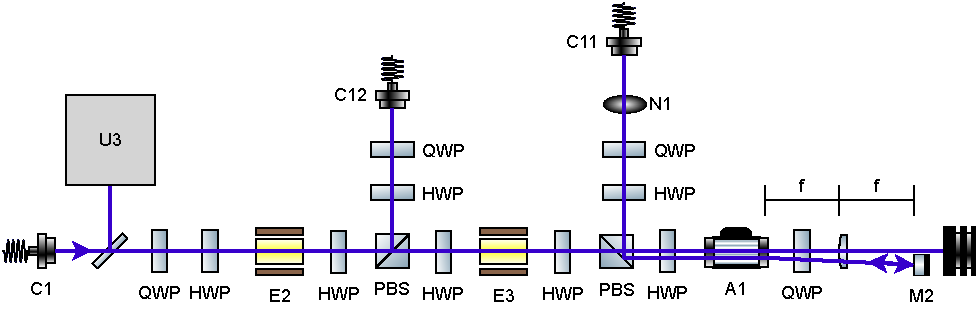
\includegraphics[width=0.8\linewidth]{fig_3_optical_path_370_modulate.pdf}
    \caption{Optical layout of laser modulation system.}
    \label{fig:fig_3_optical_path_370_modulate}
\end{figure}

Experimentally, I need to add sidebands to the 370 nm laser, the 14.7 GHz sideband (E2) for Doppler cooling and the 2.105 GHz sideband (E3) for optical pumping. The electro-optic modulator (EOM) can implement these features \cite{RN205,RN230,RN277}. The frequency and modulation depth of the sidebands can be controlled by controlling the frequency and amplitude of the EOM input microwave signal. In addition, I need to control the frequency shift and power of the 370 nm laser. This is because the difference in frequency required for Doppler cooling and state detection is approximately 12 MHz, and the frequency variation measured during calibration of the system can be compensated for by adjusting the frequency shift of the 370 nm laser \cite{RN144, RN141}. The acousto-optic modulator (AOM) provides these features. By controlling the frequency and amplitude of the microwave signal input to the AOM (A1) the frequency of the laser shift and the laser power can be controlled. However, the AOM modulation efficiency is affected by the microwave signal, as shown in Fig~\ref{fig:fig_3_optical_path_370_modulate_aom}, and we need to compensate for this using software control during experimental operation.

\begin{figure}
    \centering
    \subcaptionbox{Laser intensity versus microwave power.\label{fig:fig_3_optical_path_370_modulate_aom_power}}
    {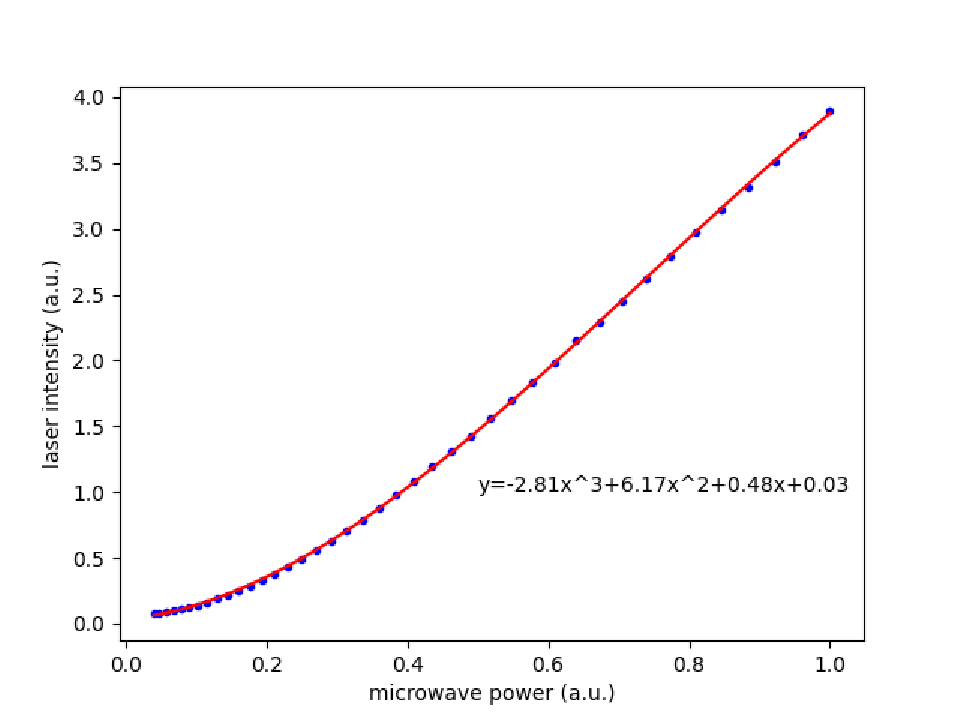
\includegraphics[width=0.4\linewidth]{fig_3_optical_path_370_modulate_aom_power.pdf}}
    \subcaptionbox{Laser intensity versus microwave frequency.\label{fig:fig_3_optical_path_370_modulate_aom_frequency}}
    {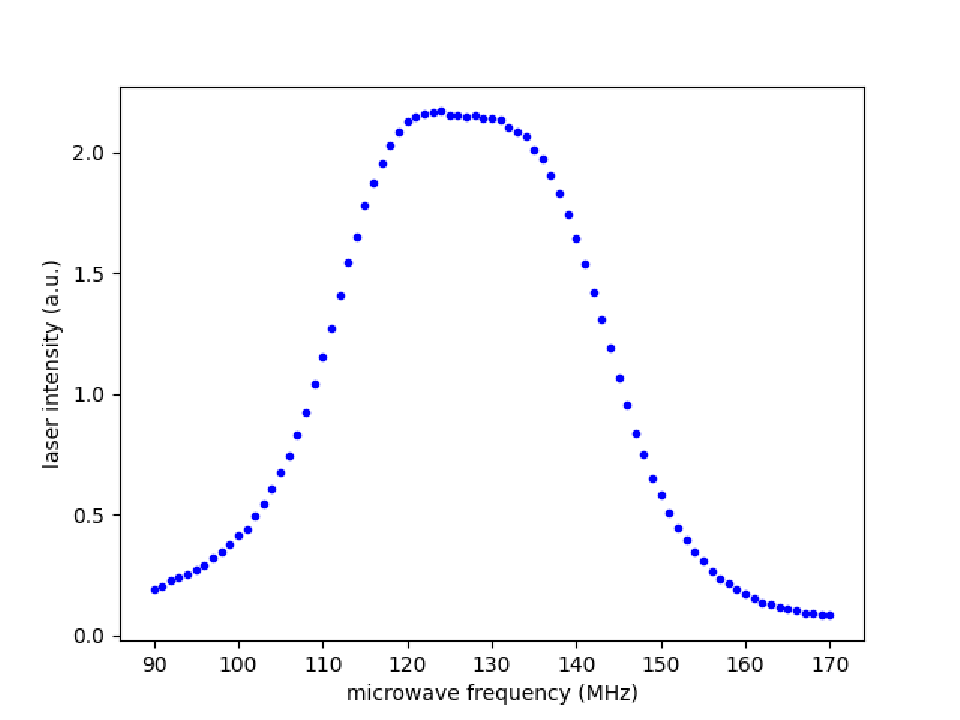
\includegraphics[width=0.4\linewidth]{fig_3_optical_path_370_modulate_aom_frequency.pdf}}
    \caption{AOM modulation efficiency influenced by microwave signal.}
    \label{fig:fig_3_optical_path_370_modulate_aom}
\end{figure}

The light source from the 370 nm laser is fed to the laser modulation module via a single-mode polarization-maintaining fibre (C1), which is reflected by a beam sampling mirror and enters the laser monitoring module (U3). A number of signal acquisition modules are integrated into the laser monitoring module to help me monitor the quality of the light source over time, including measurements of power, polarisation, laser mode and others. The main light source is modulated by two cascaded EOMs, the modulation depth of which can be maximised by adjusting the HWP. Part of the laser is coupled into the fibre (C12), which is then used for sympathetic cooling. To achieve the frequency shift, I built a double-pass configuration based on a 4f optical system, where the PBS serves to separate the incident light from the returned light by 90°, adjusting the HWP at the front to maximise the efficiency of the incident light and the HWP at the back to maximise the efficiency of the diffraction from the AOM. When the laser passes through the AOM, 0 order light is discarded and +1 order light is returned to the AOM by a 4f optical system consisting of a lens and a D-shaped pickoff mirror. The +1 order beam from the reflected beam passes through the QWP twice and is then reflected by the PBS into the fibre (C11), this light is then used for global cooling, pumping and detection. There is a mechanical shutter (N1) in front of the fibre, which serves to completely shut off the light and reduce leakage.

\subsection{Optical layout of the cryostat breadboard}

\begin{figure}
    \centering
    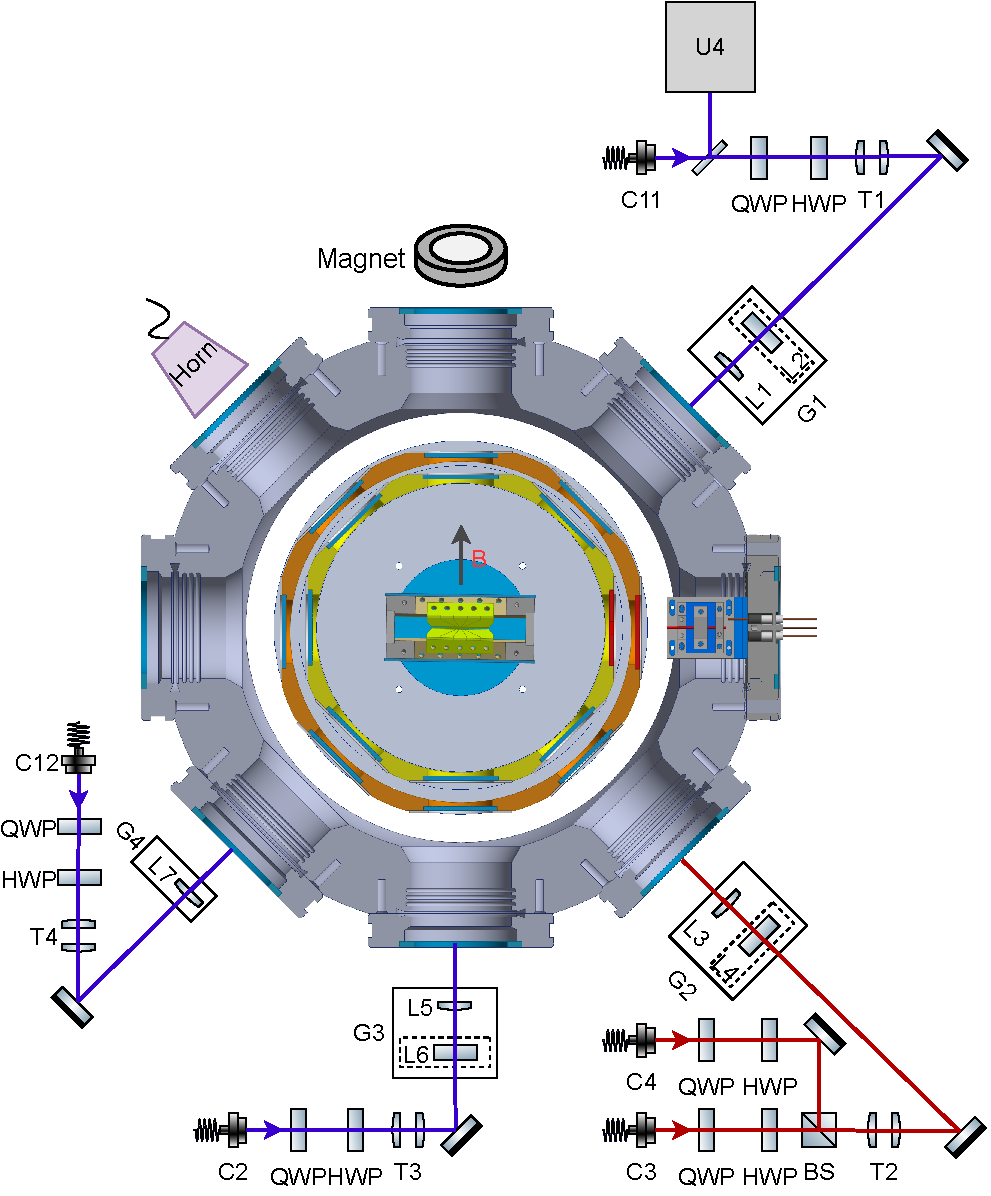
\includegraphics[width=0.8\linewidth]{fig_3_optical_path_cryostat_breadboard.pdf}
    \caption{Optical layout of the cryostat breadboard.}
    \label{fig:fig_3_optical_path_cryostat_breadboard}
\end{figure}

Due to the large base area of the cryostat, the area left for the optical path on the breadboard is relatively small. Further experimental tasks may be restricted by the number of windows. For example EIT cooling, which is important for ground state cooling in multi-ion experiments \cite{RN155, RN7, RN35, RN54}. The main function of the optical path built on the breadboard of the cryostat is to shape the beam into a specific shape and then inject it into the cavity. There are four windows on the Cryostat that are used to inject the laser. The laser light exiting the fibre collimator (C2, C3, C4, C11, C12) is first polarised by the QWP and HWP and then expanded by the lens pairs (T1, T2, T3, T4) to a suitable spot size, typically with a Gaussian diameter of approximately 10 mm. It is then incident on a long-focus lens (L1, L3, L5, L7) into the cavity and forms a small spot in the centre of the trap, typically with a Gaussian diameter of about 20 $\mu$m. The long-focus lenses are mounted on a 3-axis linear stage (G1, G2, G3, G4; M-461-XYZ-M, Newport) with a Picomotor actuator (8301NF, Newport) in each axis of the stage to achieve high precision control of the beam position.

\begin{figure}
    \centering
    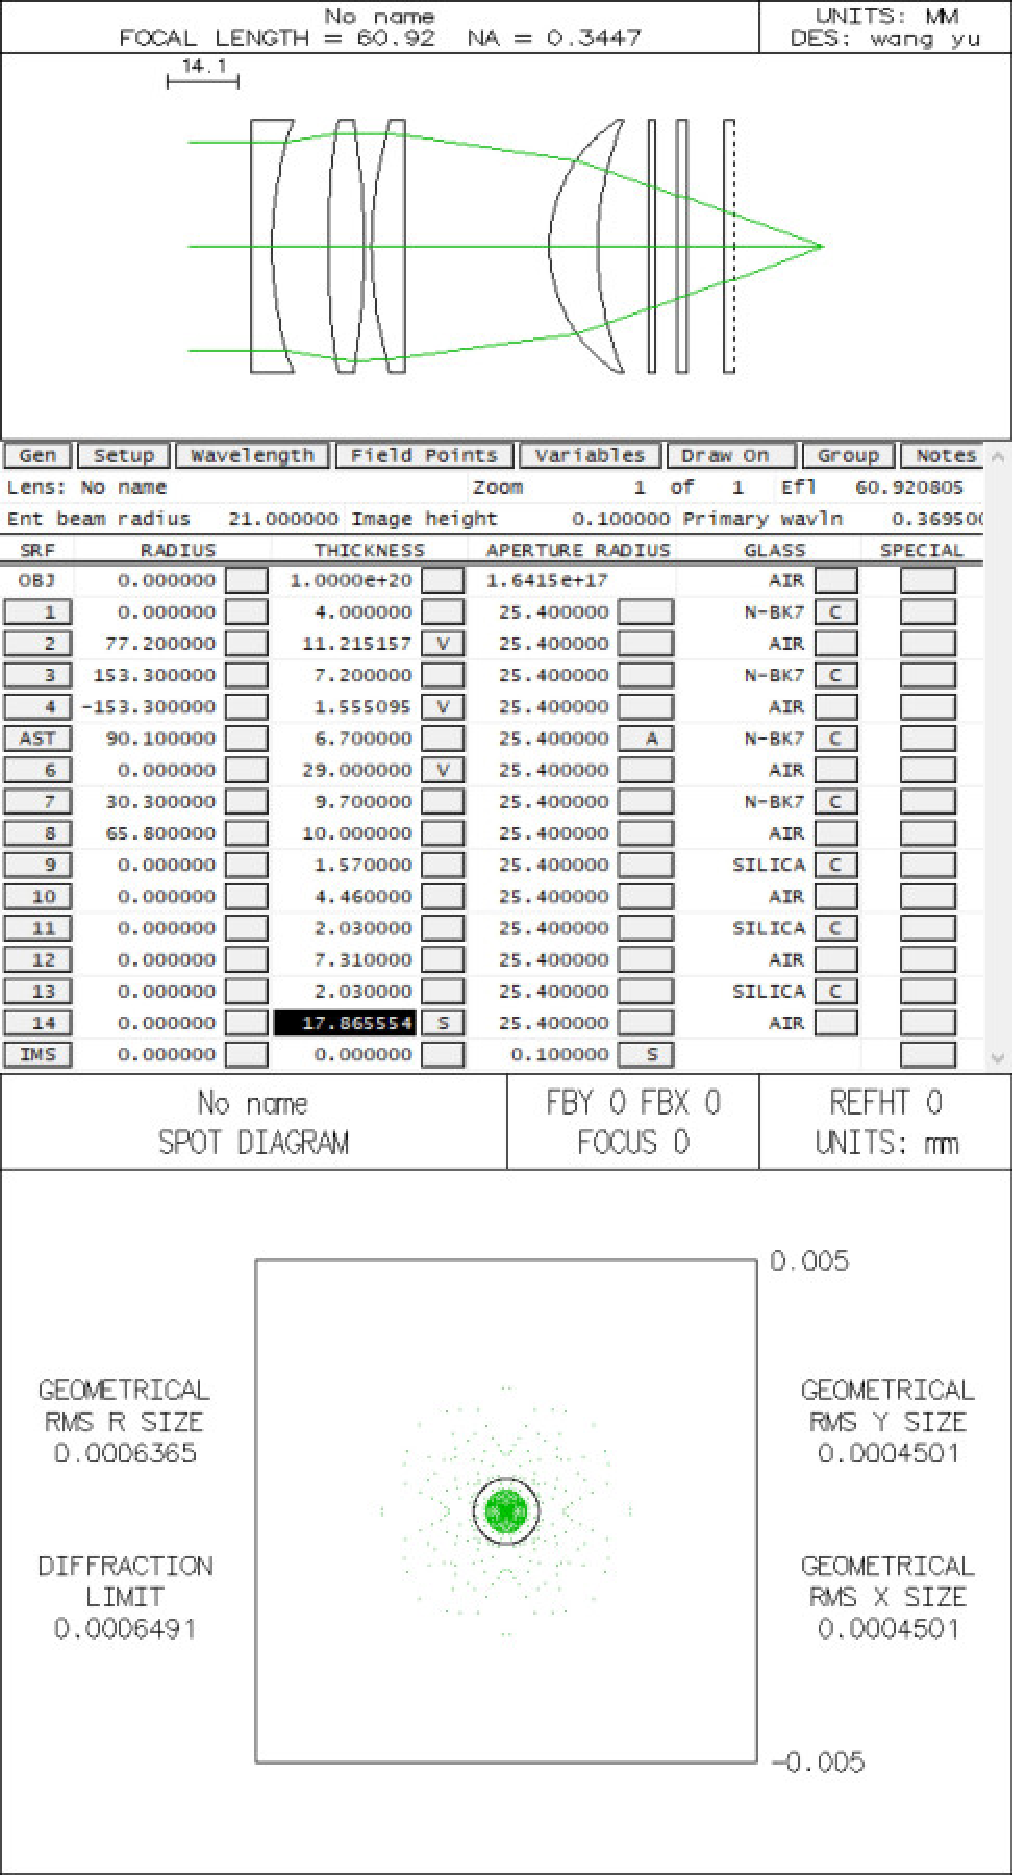
\includegraphics[width=0.4\linewidth]{fig_3_imaging_syetem_objective_design.pdf}
    \caption{Design of the objective.}
    \label{fig:fig_3_imaging_syetem_objective_design}
\end{figure}

Reducing the spot diameter at the trap is necessary to increase the power density, reduce stray light and improve the signal to noise ratio. It also helps me to monitor the displacement of the spot relative to the ions over time, which helps me to find unstable components or modules in the system at the beginning of the construction of the system. But when the length of the ion chain in the trap increases, I need some light spots to expand in the horizontal direction to about 500 $\mu$m in diameter. It is advantageous to be able to easily adjust the spot diameter in the horizontal direction. I added cylindrical lenses (L2, L4, L6) to the optical path where I needed to adjust the horizontal diameter, and by artificially introducing astigmatism, I was able to shift the horizontal focal position along the optical axis. A long-focused cylindrical lens with a focal length of approximately 1000 mm is generally used, mounted on a rotatable lens mount so that the tilt angle of the elliptical spot can be adjusted and the cylindrical lens can be removed when the elliptical spot is not required.

The stability of the 370 nm laser (C11) is so important to the experiment that a laser monitoring module (U4) has been installed at the outgoing point of the fiber. This light is global light and is required for ion loading, Doppler cooling, optical pumping, and state detection. In order to trap both ${ }^{171} \mathrm{Yb}^{+}$ and ${ }^{174} \mathrm{Yb}^{+}$, two 935 nm lasers (C3 and C4) were combined into the cavity and their function was rupumping. Combining these two 935 nm lasers at the front stage would have been a better option, but this was not done due to space planning in the laboratory. The 399 nm laser (C2) is used for ion loading and the 370 nm laser (C12) is used for sympathetic cooling.

A permanent magnet is placed in front of one window to generate a magnetic field at the centre of the trap, approximately 5 Gauss, perpendicular to the direction of the ion chain. A horn is placed in front of one of the windows to apply microwaves.

\subsection{Imaging system}

The objective is specifically designed for cryogenic trap system to collect fluorescence from the ions. The thickness of the glass inside the chamber is 5.63 mm. The numerical aperture of the fluorescence collection objective has to be as large as possible and the currently used objective has a numerical aperture of approximately 0.35. The design of the objective is shown in Fig~\ref{fig:fig_3_imaging_syetem_objective_design}

We use the PMT (Hamamatsu H11890) for State Detection of one single ion and the EMCCD (Andor iXon Ultra 888) for State Detection of multiple ions, where the average SPAM error is 3\%.

\begin{figure}
    \centering
    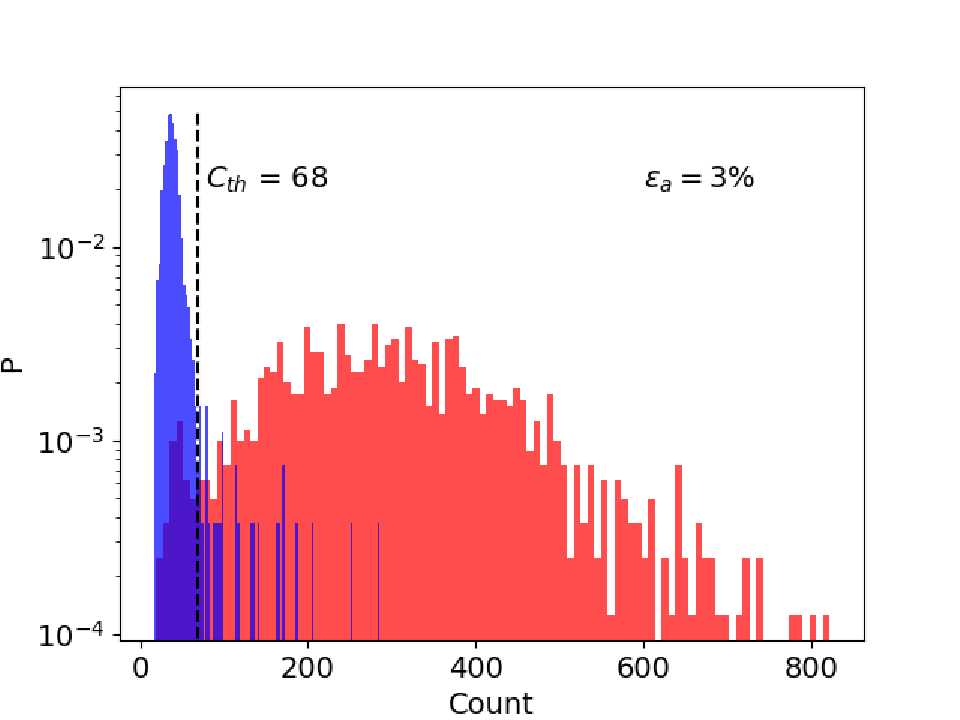
\includegraphics[width=0.5\linewidth]{fig_3_imaging_syetem_spam_error.pdf}
    \caption{Detection error analysis.}
    \label{fig:fig_3_imaging_syetem_spam_error}
\end{figure}




\section {Coherent microwaves}

\begin{table}
    \centering
    \caption{Measurement of microwave frequency and rabi rate.}
    \begin{tabular}{lll}
        \toprule
        Energy level   & microwave frequency & $\pi$-time \\
        \midrule
        $|1,0\rangle$  & 200.0344 MHz        & 122.3      \\
        $|1,-1\rangle$ & 188.0974 MHz        & 78.3       \\
        $|1,1\rangle$  & 211.9524 MHz        & 78.2       \\
        \bottomrule
    \end{tabular}
    \label{tab:microwave}
\end{table}

The system is outfitted with a microwave horn in order to coherently drive global spin rotations.
The $|\downarrow\rangle$ and $|\uparrow\rangle$ states are directly coupled by a magnetic dipole moment, so the
microwaves can directly drive rotations. Microwave signals are generated by mixing high frequency signals (Rohde \& Schwarz SMB-100A, 11 dBm @ 12.4428 GHz) with low frequency signals (Analog Devices AD9910, around 200 MHz). The signals then passes through a high frequency amplifier and is output to a microwave speaker. Measurement of microwave frequency and rabi rate for different energy levels is shown in Table~\ref{tab:microwave}. Here the microwave frequency is added to 12.4428 Ghz to get the absolute frequency of the corresponding energy level.
